\chapter{\chapternameanalysis}\label{analise}
Neste capítulo, apresentamos a análise das galáxias ultracompactas (UCDs) no aglomerado de Fornax, com foco nas propriedades das UCDs conhecidas e na seleção de novas candidatas. Inicialmente, discutimos as características das UCDs previamente identificadas e sua distribuição espacial. Em seguida, exploramos a relação entre as UCDs e as galáxias massivas do aglomerado. Também detalhamos o uso de aprendizado de máquina para classificar objetos compactos e extensos, além de calcular redshifts fotométricos para refinar a seleção de candidatas. Por fim, apresentamos a amostra final de candidatas a UCDs e realizamos uma análise comparativa com as UCDs conhecidas e galáxias morfologicamente classificadas.

\section{UCDs em Fornax}\label{sec:ucds_fornax}
Em uma análise inicial, observamos as propriedades das UCDs conhecidas de Fornax na nossa amostra. Utilizamos o catálogo de UCDs conhecidas de \cite{catalog_ucds}, que compila descobertas de outros trabalhos até o ano de sua publicação. Na Figura \ref{distribution_know_ucds}, apresentamos a distribuição espacial das UCDs desse catálogo na região de Fornax. Na Figura \ref{distribuicao_ucds_center} apresentamos a distribuição dessas UCDs apenas na região de Fornax

\begin{figure}[!ht]
    \centering
    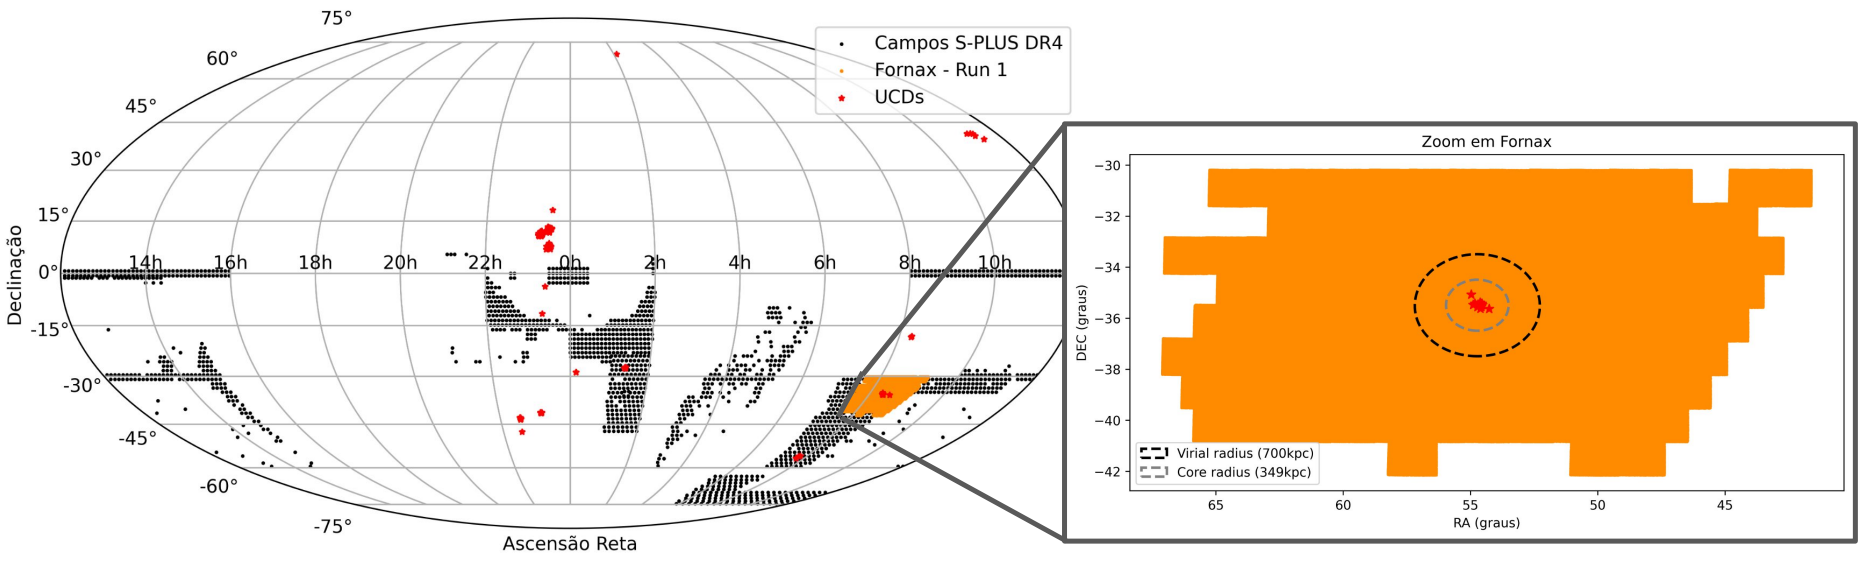
\includegraphics[width=1.\columnwidth,angle=0]{distribution_know_ucds.png}
    \caption[]{Distribuição dos campos observados do S-PLUS DR4 no céu em coordenadas equatoriais. Os pontos pretos representam os campos do S-PLUS DR4, enquanto os pontos azuis indicam as UCDs selecionadas como conhecidas vindas de \cite{catalog_ucds}. A área em laranja corresponde ao Aglomerado de Fornax com a redução da fotometria vinda de \cite{haack2024splusfornaxprojectsfp}, denominados \textit{Run 1}. As linhas de grade mostram a Ascensão Reta (em horas) e Declinação (em graus). A imagem mais ao lado é um zoom da região de Fornax.}
    \label{distribution_know_ucds}
\end{figure}

Os objetos compilados presentes na nossa amostra de Fornax tiveram suas propriedades estudadas por \cite{Mieske_2008_2}, onde todos os alvos foram confirmados como pertencentes ao aglomerado por meio de pesquisas espectroscópicas (\citealt{Drinkwater_2000}, \citealt{Mieske_2002} \& \citeyear{Mieske_2004}, \citealt{Richtler_2004} \& \citeyear{Richtler_2008}). Dessas descobertas, as 5 primeiras UCDs (chamadas de UCDs clássicas) foram encontradas em Fornax por \cite{Drinkwater_2000}.

Dessas lista de UCDs, com 18 na região de Fornax, foi feito um cruzamento com os dados utilizados neste trabalho. Obtivemos 16 objetos correspondentes na nossa amostra. Na Tabela \ref{ucds_fornax_propriedades}, apresentamos a lista dessas UCDs conhecidas e suas propriedades fornecidas por \citealt{Mieske_2008_2}.

\begin{table}[!ht]
    \centering
    \caption{Propriedades das UCDs identificadas na região de Fornax com dados da amostra deste estudo, fornecidas por \citealt{Mieske_2008_2}. As colunas representam: Nome - identificação do objeto; RA - Ascensão Reta em graus; Dec - Declinação em graus; Massa Total - massa total do objeto em $10^6 \, M_\odot$; $M/L_V$ - razão massa-luminosidade; [Fe/H] - metalicidade em dex; $r_h$ - raio de meia-luz em parsecs (com relação à banda V); $\sigma$ - dispersão de velocidade em km/s.}
    \begin{tabular}{lcccccccc}
        \toprule
        Nome & RA & Dec & Massa Total & $M/L_V$ & [Fe/H] & $r_h$ & $\sigma$ \\
        & (graus) & (graus) & ($10^6 \, M_\odot$) & & (dex) & (pc) & (km/s)\\
        \midrule
        UCD3, F-19 & 54.72542 & -35.55933 & $93.6 \pm 14.0$ & $4.69 \pm 0.70$ & -0.4 & 89.7 & 22.8 \\
        UCD1       & 54.26375 & -35.63461 & $32.1 \pm 3.9$  & $4.99 \pm 0.60$ & -0.7 & 22.4 & 27.1 \\
        F-24       & 54.89958 & -35.47350 & $24.5 \pm 7.8$  & $3.44 \pm 1.10$ & -0.4 & 29.5 & 21.4 \\
        UCD5       & 54.96908 & -35.07336 & $18.0 \pm 4.5$  & $3.37 \pm 0.85$ & -1.2 & 31.2 & 18.7 \\
        F-1a       & 54.52625 & -35.48300 & $16.2 \pm 3.8$  & $2.45 \pm 0.58$ & 0.0  & 23.1 & 18.7 \\
        F-9        & 54.60625 & -35.62853 & $14.1 \pm 3.6$  & $4.72 \pm 1.20$ & -0.8 & 9.1  & 25.7 \\
        F-5        & 54.54500 & -35.42950 & $13.7 \pm 2.4$  & $3.16 \pm 0.55$ & -0.3 & 5.0  & 34.5 \\
        F-6        & 54.56875 & -35.43878 & $12.5 \pm 2.4$  & $5.32 \pm 1.00$ & 0.2  & 7.3  & 27.3 \\
        F-7        & 54.57333 & -35.55067 & $10.5 \pm 1.4$  & $4.21 \pm 0.57$ & -1.3 & 14.9 & 20.1 \\
        F-12       & 54.62083 & -35.38231 & $8.3 \pm 2.9$   & $2.36 \pm 0.83$ & -0.4 & 10.3 & 22.9 \\
        F-11       & 54.61792 & -35.42736 & $5.7 \pm 3.7$   & $1.64 \pm 1.10$ & -0.9 & 3.6  & 26.2 \\
        F-34       & 54.55292 & -35.48250 & $5.5 \pm 1.3$   & $3.17 \pm 0.74$ & -0.9 & 4.0  & 24.6 \\
        F-22       & 54.82375 & -35.42503 & $5.3 \pm 1.0$   & $2.13 \pm 0.39$ & -0.4 & 10.0 & 22.8 \\
        F-53       & 54.66917 & -35.48611 & $3.9 \pm 1.0$   & $2.66 \pm 0.69$ & -0.9 & 4.4  & 19.6 \\
        F-51       & 54.57125 & -35.44203 & $3.5 \pm 0.9$   & $2.38 \pm 0.62$ & -0.8 & 4.2  & 20.1 \\
        F-59       & 54.70375 & -35.46225 & $1.3 \pm 0.6$   & $0.94 \pm 0.43$ & -2.1 & 5.7  & 9.8  \\
        \bottomrule
    \end{tabular}
    \label{ucds_fornax_propriedades}
\end{table}

Fazendo um cruzamento das UCDs conhecidas do catálogo de \cite{catalog_ucds} com os dados da fotometria original do S-PLUS DR4, obtivemos 9 objetos, em comparação com os 16 que obtivemos anteriormente. Isso ressalta a importância da redução da fotometria de Fornax vinda de \cite{haack2024splusfornaxprojectsfp} para a identificação das nossas galáxias de interesse.

Fazendo um cruzamento dessas UCDs conhecidas nos nossos dados com o catálogo GAIA DR3 \citep{GAIA_DR3}, que fornece informações de classificação estrela-galáxia-quasar, observamos que das 16, 8 têm probabilidade maior que 50\% de serem galáxias e 8 têm probabilidade maior que 50\% de serem estrelas. Esse fato mostra a dificuldade de parte da classificação desses objetos. Mostramos na Tabela \ref{tab_ucds_stars_galaxy_like} as médias e desvios padrões das magnitudes dos dados usados desses dois grupos.

\begin{table}[!ht]
    \centering
    \caption{Comparação das 12 magnitudes do S-PLUS DR4 (Run 1) da abertura APER\_6 corrigidas pela extinção entre as UCDs conhecidas, separadas em dois grupos: classificação estrela (PSS > 0,5) ou galáxia (PGal > 0,5) pelo Gaia DR3.}   
    \begin{tabular}{lcccc}
        \toprule
        Filtro & \multicolumn{2}{c}{UCD(PGal>0,5)} & \multicolumn{2}{c}{UCD(PSS>0,5)} \\
        & Média & $\sigma$ & Média & $\sigma$ \\
        \midrule
        u & 21,73 & 0,83 & 22,03 & 0,37 \\
        J0378 & 21,13 & 0,84 & 22,04 & 0,49 \\
        J0395 & 21,29 & 1,04 & 22,42 & 1,23 \\
        J0410 & 20,41 & 0,53 & 21,63 & 0,57 \\
        J0430 & 20,29 & 0,67 & 21,16 & 0,33 \\
        g    & 19,88 & 0,73 & 21,07 & 0,63 \\
        J0515 & 19,60 & 0,63 & 20,75 & 0,46 \\
        r    & 18,08 & 0,67 & 20,41 & 0,36 \\
        J0660 & 19,00 & 0,68 & 20,27 & 0,39 \\
        i    & 18,75 & 0,72 & 20,10 & 0,44 \\
        J861 & 18,58 & 0,69 & 19,82 & 0,36 \\
        z    & 18,54 & 0,72 & 19,98 & 0,51 \\
        \bottomrule
    \end{tabular}
    \label{tab_ucds_stars_galaxy_like}
\end{table}

Concluímos pela Tabela \ref{tab_ucds_stars_galaxy_like} que o grupo de UCDs classificadas como galáxias pelo GAIA DR3 é mais brilhante que o grupo classificado como estrelas. Observando ainda a banda fotométrica $r$, usada como referência devido à sua profundidade e qualidade, temos as UCDs classificadas como galáxias no intervalo de 17,64 a 19,83 magnitudes, enquanto as classificadas como estrelas estão no intervalo de 19,8 a 20,83 magnitudes. Podemos usar estes intervalos como referência para a seleção dos objetos de interesse.

Pelas propriedades da Tabela \ref{ucds_fornax_propriedades}, mostramos na Figura \ref{r_h_M_ucds} a relação entre a massa e o raio de meia-luz das UCDs conhecidas de Fornax. Observamos uma conclusão similar: o grupo de UCDs classificadas como galáxias pelo GAIA DR3 é mais brilhante que o grupo classificado como estrelas, e assim, tem uma relação entre a massa e o raio de meia-luz maior.

\begin{figure}[!ht]
    \centering
    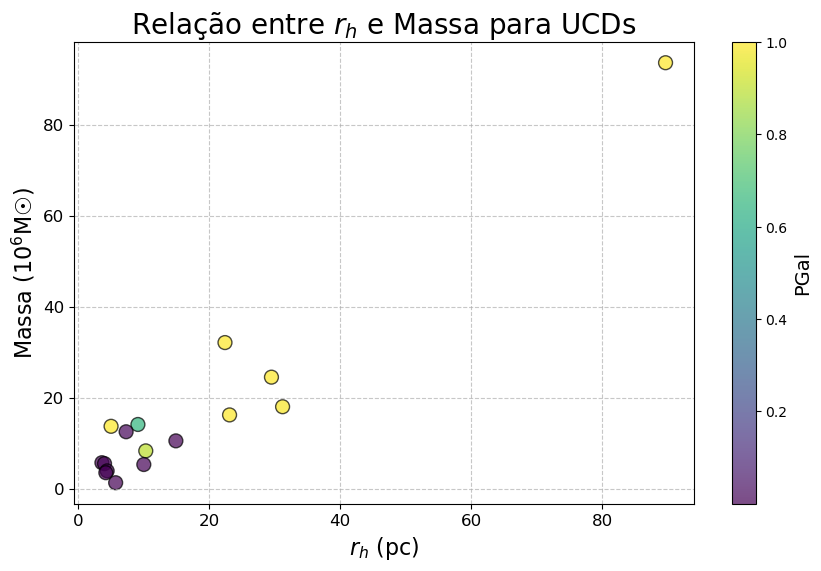
\includegraphics[width=0.8\columnwidth,angle=0]{r_h_M_ucds.png} 
    \caption[]{Relação entre a massa e o raio de meia-luz das UCDs conhecidas de Fornax. Barra de cor pela classificação como galáxia (PGal) vinda do Gaia DR3.}
    \label{r_h_M_ucds}
\end{figure}

Na Figura \ref{distribuicao_fwhm_image_r_r_aper6_ucds_fornax}, mostramos a distribuição de \textit{FWHM (r-band)} em função da banda \textit{r\_APER\_6} para UCDs de Fornax, coloridas pelo classificador de galáxia (PGal) do Gaia DR3. Percebemos que, para os objetos mais fracos, o classificador do Gaia apresenta maior taxa de erro ao classificá-los, atribuindo maiores probabilidades de serem estrelas. A UCD \textit{F-34} é a que possui o maior valor de \textit{FWHM}. Observando as imagens, não notamos que ela seja significativamente maior que as outras. No entanto, possivelmente devido à sua proximidade com o centro do aglomerado, em uma região onde a magnitude na banda \textit{r} é mais alta, sua fotometria pode ser afetada por outros objetos próximos, aumentando ligeiramente o seu \textit{FWHM} nas detecções.

\begin{figure}[!ht]
    \centering
    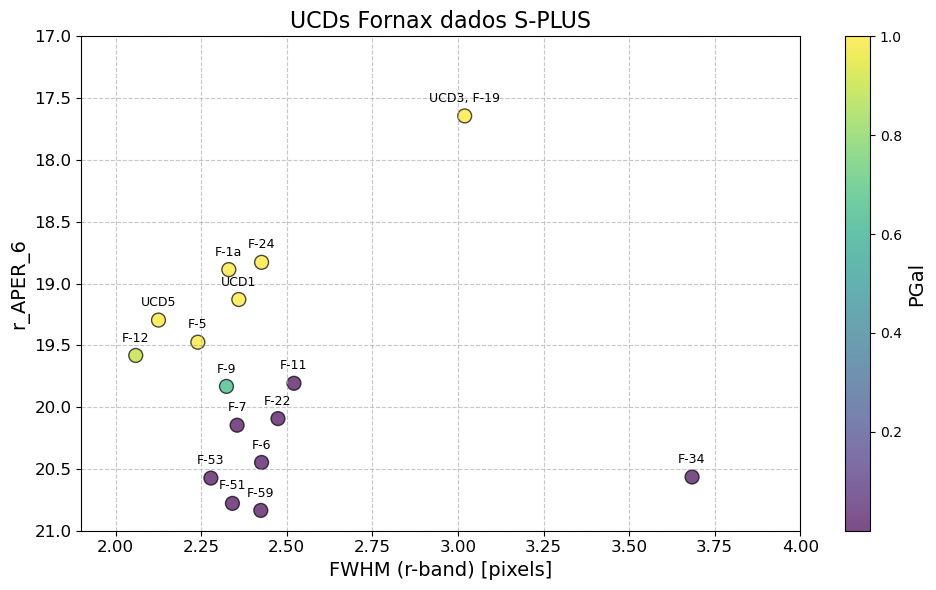
\includegraphics[width=0.8\columnwidth,angle=0]{distribuicao_fwhm_image_r_r_aper6_ucds_fornax.png}
    \caption[]{Distribuição de \textit{FWHM (r-band)} em função da magnitude \textit{r\_APER\_6} para UCDs de Fornax nos dados do S-PLUS.}
    \label{distribuicao_fwhm_image_r_r_aper6_ucds_fornax}
\end{figure}

Usando o compilado de redshifts espectroscópicos de \cite{Lima_2024}, mostramos na Tabela \ref{tab:ucds_know_z_gmag} os valores para esses objetos catalogados como UCDs em nossos dados, vindo de \cite{catalog_ucds}, juntamente da magnitude $g$ na abertura $APER\_6$ de referência. 

\begin{table}[!ht]
    \centering
    \caption{Valores de redshift espectroscópico ($z_{spec}$) provenientes de \cite{Lima_2024} e magnitudes $g$ e abertura $APER\_6$ obtidas dos dados fotométricos utilizados neste trabalho.}
    \begin{tabular}{lcc}
        \toprule
        Nome & $z_{spec}$ & $g_APER_6$ \\
        \midrule
        UCD3 & 0.0053 & 18.47\\
        UCD1 & 0.0052 & 19.75\\
        F-24 & 0.0063 & 19.66\\
        UCD5 & 0.0045 & 19.71\\
        F-1a & 0.0042 & 19.66\\
        F-9  & 0.0058 & 20.85\\
        F-5  & 0.0057 & 20.54\\
        F-6  & 0.0037 & 20.48\\
        F-7  & 0.0050 & 20.89\\
        F-12 & 0.0055 & 20.37\\
        F-11 & 0.0059 & 20.40\\
        F-34 & 0.0054 & 20.79\\
        F-22 & 0.0034 & 20.69\\
        F-53 & 0.0020 & 21.57\\
        F-51 & 0.0041 & 22.23\\
        F-59 & 0.0061 & 21.47\\
        \bottomrule
    \end{tabular}
    \label{tab:ucds_know_z_gmag}
\end{table}

Com base na Tabela \ref{tab:ucds_know_z_gmag}, e conforme definido na seção \ref{subsec:cuts}, consideraremos como UCDs os objetos com magnitudes $g$ menores que 21. Dessa forma, para as análises comparativas da amostra final de candidatas a UCDs, iremos remover os objetos confirmados de Fornax que possuem magnitudes aparentes mais altas, pois, mesmo sendo objetos compactos, seriam categorizados como aglomerados globulares.

\subsection{Distribuição relativa ao centro de Fornax}
Na Figura \ref{distribuicao_ucds_center}, apresentamos a distribuição de UCDs conhecidas nos dados do S-PLUS, com respeito ao centro do aglomerado. No centro do aglomerado, temos a galáxia NGC 1399, que é a galáxia mais massiva do aglomerado de Fornax.

\begin{figure}[!ht]
    \begin{center}
    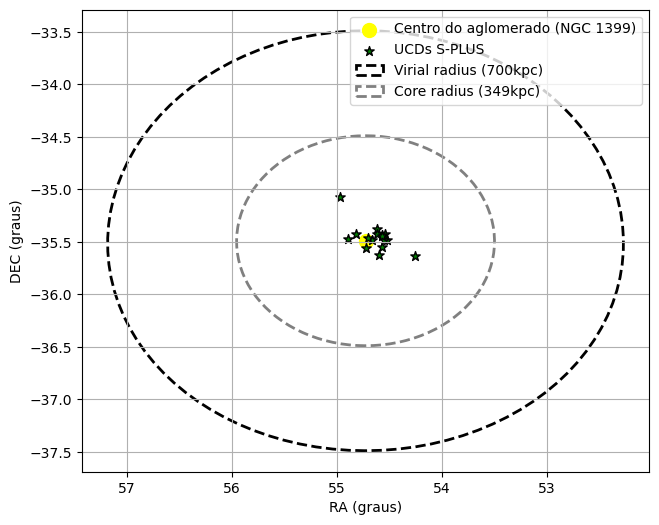
\includegraphics[width=0.9\columnwidth,angle=0]{distribuicao_ucds_center.png}
    \caption[]{Distribuição das UCDs conhecidas de Fornax nos dados do S-PLUS. Os pontos azuis representam as UCDs conhecidas, coloridas pelo raio de virial (virial radius) e o raio do núcleo (core radius). Centro do aglomerado representado pelo círculo amarelo (NGC 1399), em RA = 54.73 e Dec = -35.49.}
    \label{distribuicao_ucds_center}
    \end{center}
\end{figure}

Nesta figura, apresentamos a distribuição das UCDs nos dados do S-PLUS, destacando o raio de virial ($virial \, radius$) e o raio do núcleo ($core \, radius$). Utilizamos o $virial \, radius$ como 700 kpc \citep{Drinkwater_2001} e definimos o $core \, radius$ como aproximadamente 349 kpc, assim como feito por \cite{Saifollahi_2021}, o que corresponde a 1 grau no céu (aproximadamente metade do raio de virial). Essa representação evidencia que os objetos estão ainda mais concentrados no centro do aglomerado.

Para a conversão de kpc para graus, usamos a relação:

\begin{equation}
    \theta = \frac{d}{D} \times \frac{180}{\pi}
\end{equation}
onde $d$ é o tamanho em kpc, $D$ é a distância em kpc até o objeto, e $\theta$ é o tamanho em graus. Considerando que Fornax está a aproximadamente $20 \, \text{Mpc}$ \citep{Blakeslee_2009}, o que corresponde a um módulo de distância de $31.51 \, \text{mag}$, nessa distância, 1 grau equivale a $0.349 \, \text{Mpc}$. Assim, para as propriedades de Fornax, adotamos os valores apresentados na Tabela \ref{tab:properties_fornax}.

% \begin{table}[!ht]
%     \centering    
%     \caption{Propriedades do aglomerado de Fornax. As referências são indicadas por números sobrescritos nos parâmetros: ¹\citealp{Drinkwater_2001}, ²\citealp{Blakeslee_2009}, ³\citealp{Maddox_2019}, ⁴\citealp{Saifollahi_2021}.}   
%     \begin{tabular}{lc}
%         \toprule
%         Parâmetro &  Valor\\
%         \midrule
%         Massa ($M_\odot$)¹ & $7\pm 2. 10^{13}$ \\
%         Raio Virial ($Mpc$)¹ & 0.7 \\
%         Raio Virial ($graus$)¹ & 2 \\
%         Raio interno ($Mpc$)⁴ & 0.349 \\
%         Raio interno ($graus$)⁴ & 1 \\
%         Dispersão de velocidade ($km s^{-1}$)³ & 318 \\
%         Modulo de distância ($mag$)² & 31.51 \\
%         \bottomrule
%     \end{tabular}
%     \label{tab:properties_fornax}
% \end{table}


\begin{table}[!ht]
    \centering    
    \caption{Propriedades do aglomerado de Fornax. As referências são indicadas por números sobrescritos nos parâmetros: $^1$\citealp{Drinkwater_2001}, $^2$\citealp{Blakeslee_2009}, $^3$\citealp{Maddox_2019}. Definição do termo \textit{Raio interno (virial core)} feita vinda de $^4$\cite{Saifollahi_2021}..}   
    \begin{tabular}{lc}
        \toprule
        Parâmetro &  Valor\\
        \midrule
        Massa ($M_\odot$)$^1$ & $7\pm 2. 10^{13}$ \\
        Raio Virial ($Mpc$)$^1$ & 0.7 \\
        Raio Virial ($graus$)$^1$ & 2 \\
        Raio interno ($Mpc$)$^4$ & 0.349 \\
        Raio interno ($graus$)$^4$ & 1 \\
        Dispersão de velocidade ($km s^{-1}$)$^3$ & 318 \\
        Modulo de distância ($mag$)$^2$ & 31.51 \\
        \bottomrule
    \end{tabular}
    \label{tab:properties_fornax}
\end{table}

Na Figura \ref{distribuicao_ucds_center}, observamos que as UCDs conhecidas estão concentradas no centro do aglomerado. A presença de UCDs no centro é consistente com outros estudos, que também identificaram essas estruturas em regiões de alta densidade de galáxias massivas. No entanto, esse padrão pode estar relacionado ao viés das pesquisas espectroscópicas, que tendem a se concentrar nas áreas centrais do aglomerado, e não necessariamente reflete a distribuição real das UCDs em Fornax.

\section{Seleção de Galáxias Massivas em Fornax}\label{subsec:galaxias_massivas}
Para ilustrar melhor a distribuição espacial das UCDs em Fornax, também é útil apresentar as regiões com a presença das principais galáxias massivas encontradas. 

A presença e a distribuição das galáxias massivas são importantes, pois, além do centro do aglomerado, onde as UCDs estão mais concentradas, as galáxias massivas também podem desempenhar um papel relevante na localização dessas estruturas. Segundo o cenário de {\it tidal stripping}, as UCDs podem ser formadas a partir da interação com uma galáxia mais massiva. Assim, quando uma galáxia anã nucleada começa a interagir com uma galáxia mais massiva, após algumas passagens orbitais, parte de sua matéria pode ser removida, resultando no núcleo remanescente, que observamos como sendo uma UCD. Mostramos então também onde as principais galáxias massivas estão localizadas no aglomerado, e como a distribuição das candidatas a UCDs se compara com a distribuição dessas galáxias.

Selecionamos os trabalhos provenientes de uma lista de referências das galáxias confirmadas do aglomerado (\citealp{Ferguson_1989}, \citealp{Jordan_2007}, \citealp{Venhola_2018}). A partir dessas listas de objetos, filtramos utilizando o catálogo de \cite{Lima_2024}, que compila redshifts espectroscópicos confirmados. Selecionamos apenas os objetos com valores presentes e dentro da faixa de redshift do aglomerado de Fornax. Para identificar as galáxias mais massivas entre esses objetos, realizamos um corte na magnitude absoluta $M_r$, utilizando a abertura de 6 arcsecs. Calculamos a magnitude absoluta com base no módulo de distância da Tabela \ref{tab:properties_fornax} e na magnitude aparente $m_r$ dos objetos.

Utilizando todos os objetos da nossa amostra de Fornax com redshift confirmado nesse mesmo intervalo, mostramos na Figura \ref{hist_mag_abs} a distribuição da magnitude absoluta $M_r$ dos objetos.

\begin{figure}[!ht]
    \centering
    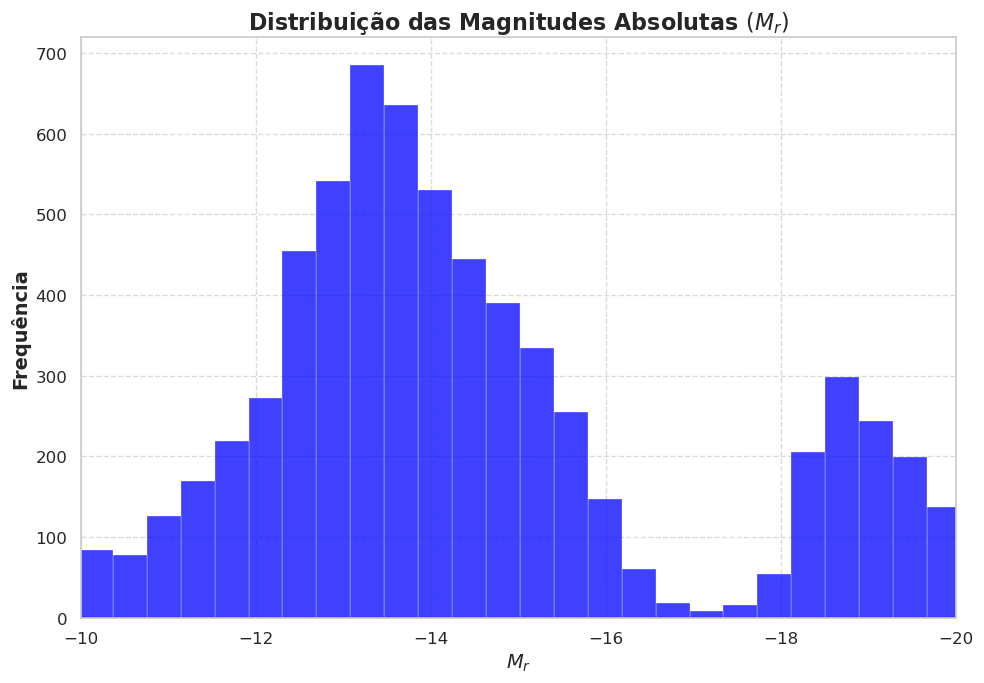
\includegraphics[width=0.7\columnwidth,angle=0]{hist_mag_abs.png}
    \caption[]{Distribuição da magnitude absoluta $M_r$ dos objetos com redshift confirmado na região de Fornax.}
    \label{hist_mag_abs}
\end{figure}

Observamos dois picos de magnitudes, um em torno de -13 e outro em torno de -19. Os dois picos na distribuição de $M_r$ têm origens distintas e estão relacionados tanto à função de luminosidade intrínseca do aglomerado de Fornax quanto aos limites de detecção do levantamento. O pico em torno de -19 coincide aproximadamente com o joelho da função de Schechter das galáxias em aglomerados: é onde a densidade de galáxias gigantes (elípticas e lenticulares do núcleo de Fornax, como NGC 1399) é mais alta antes de cair exponencialmente. O pico em torno de -13 está correlacionado ao limite de completude do catálogo para os objetos mais fracos ou mais distantes. Assim que chegamos perto do limite de detecção, o número de objetos cai abruptamente para além desse valor.

Para o regime das galáxias mais massivas, e assim mais brilhantes, selecionaremos, assim como adotado em \cite{Saifollahi_2021}, um corte em $M_r \leq -18$ para a seleção das galáxias massivas, onde estaremos considerando esse segundo pico de magnitudes. 

Na Figura \ref{distribuicao_galaxias_massivas} na imagem superior, apresentamos a distribuição espacial das galáxias massivas em Fornax. Acrescentamos em cada uma delas um raio de 200 kpc. Esse valor é comparável com o raio de virial da Via Lactea ($R_{vir}\sim 200kpc$, \cite{Dehnen_2006}). Apresentamos ainda na Figura \ref{distribuicao_galaxias_massivas}, na imagem inferior, a mesma distribuição sobreposta a uma imagem do aglomerado de Fornax, criadas com as imagens do Legacy Survey.

% \begin{figure}[!ht]
%     \centering
%     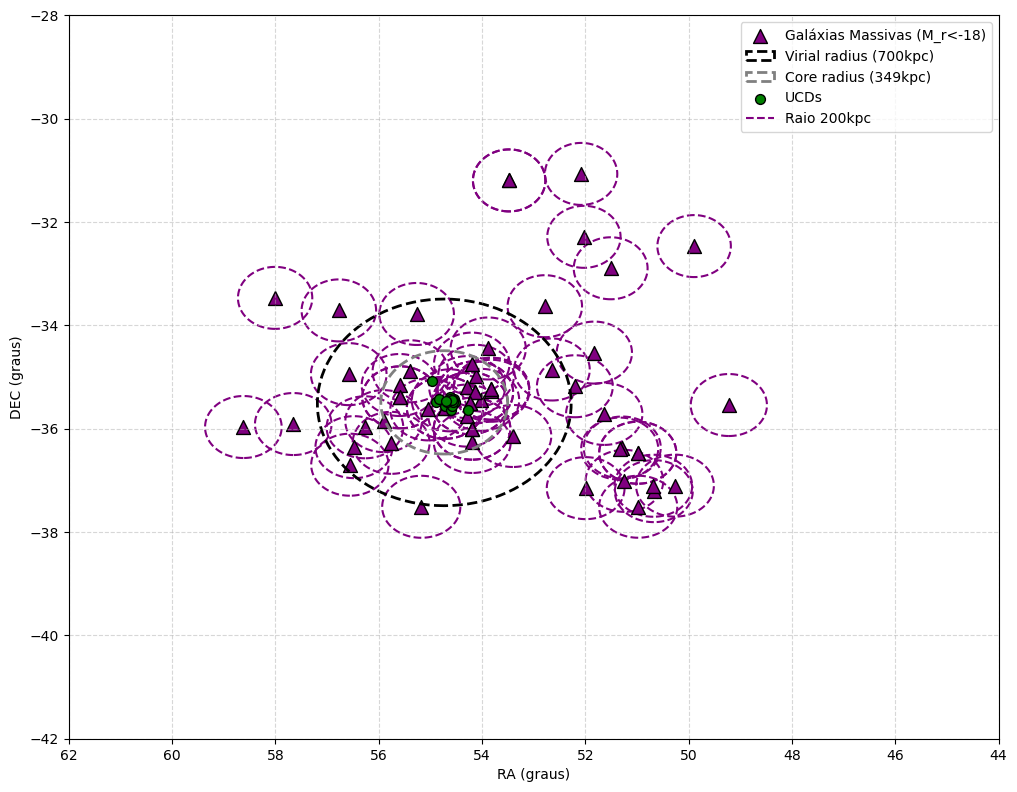
\includegraphics[width=0.6\columnwidth,angle=0]{distribuicao_galaxias_massivas.png}
%     \caption[]{Distribuição das galáxias massivas em Fornax nos dados do S-PLUS. Os pontos em roxo representam as galáxias massivas, com um círculo indicando um raio de 200 kpc ao redor de cada uma. O arco preto corresponde ao raio de virial de Fornax, estimado em 700 kpc, enquanto o arco cinza representa o raio do núcleo (core radius), definido como 349 kpc.}
%     \label{distribuicao_galaxias_massivas}
% \end{figure}


% \begin{figure}[!ht]
%     \centering
%     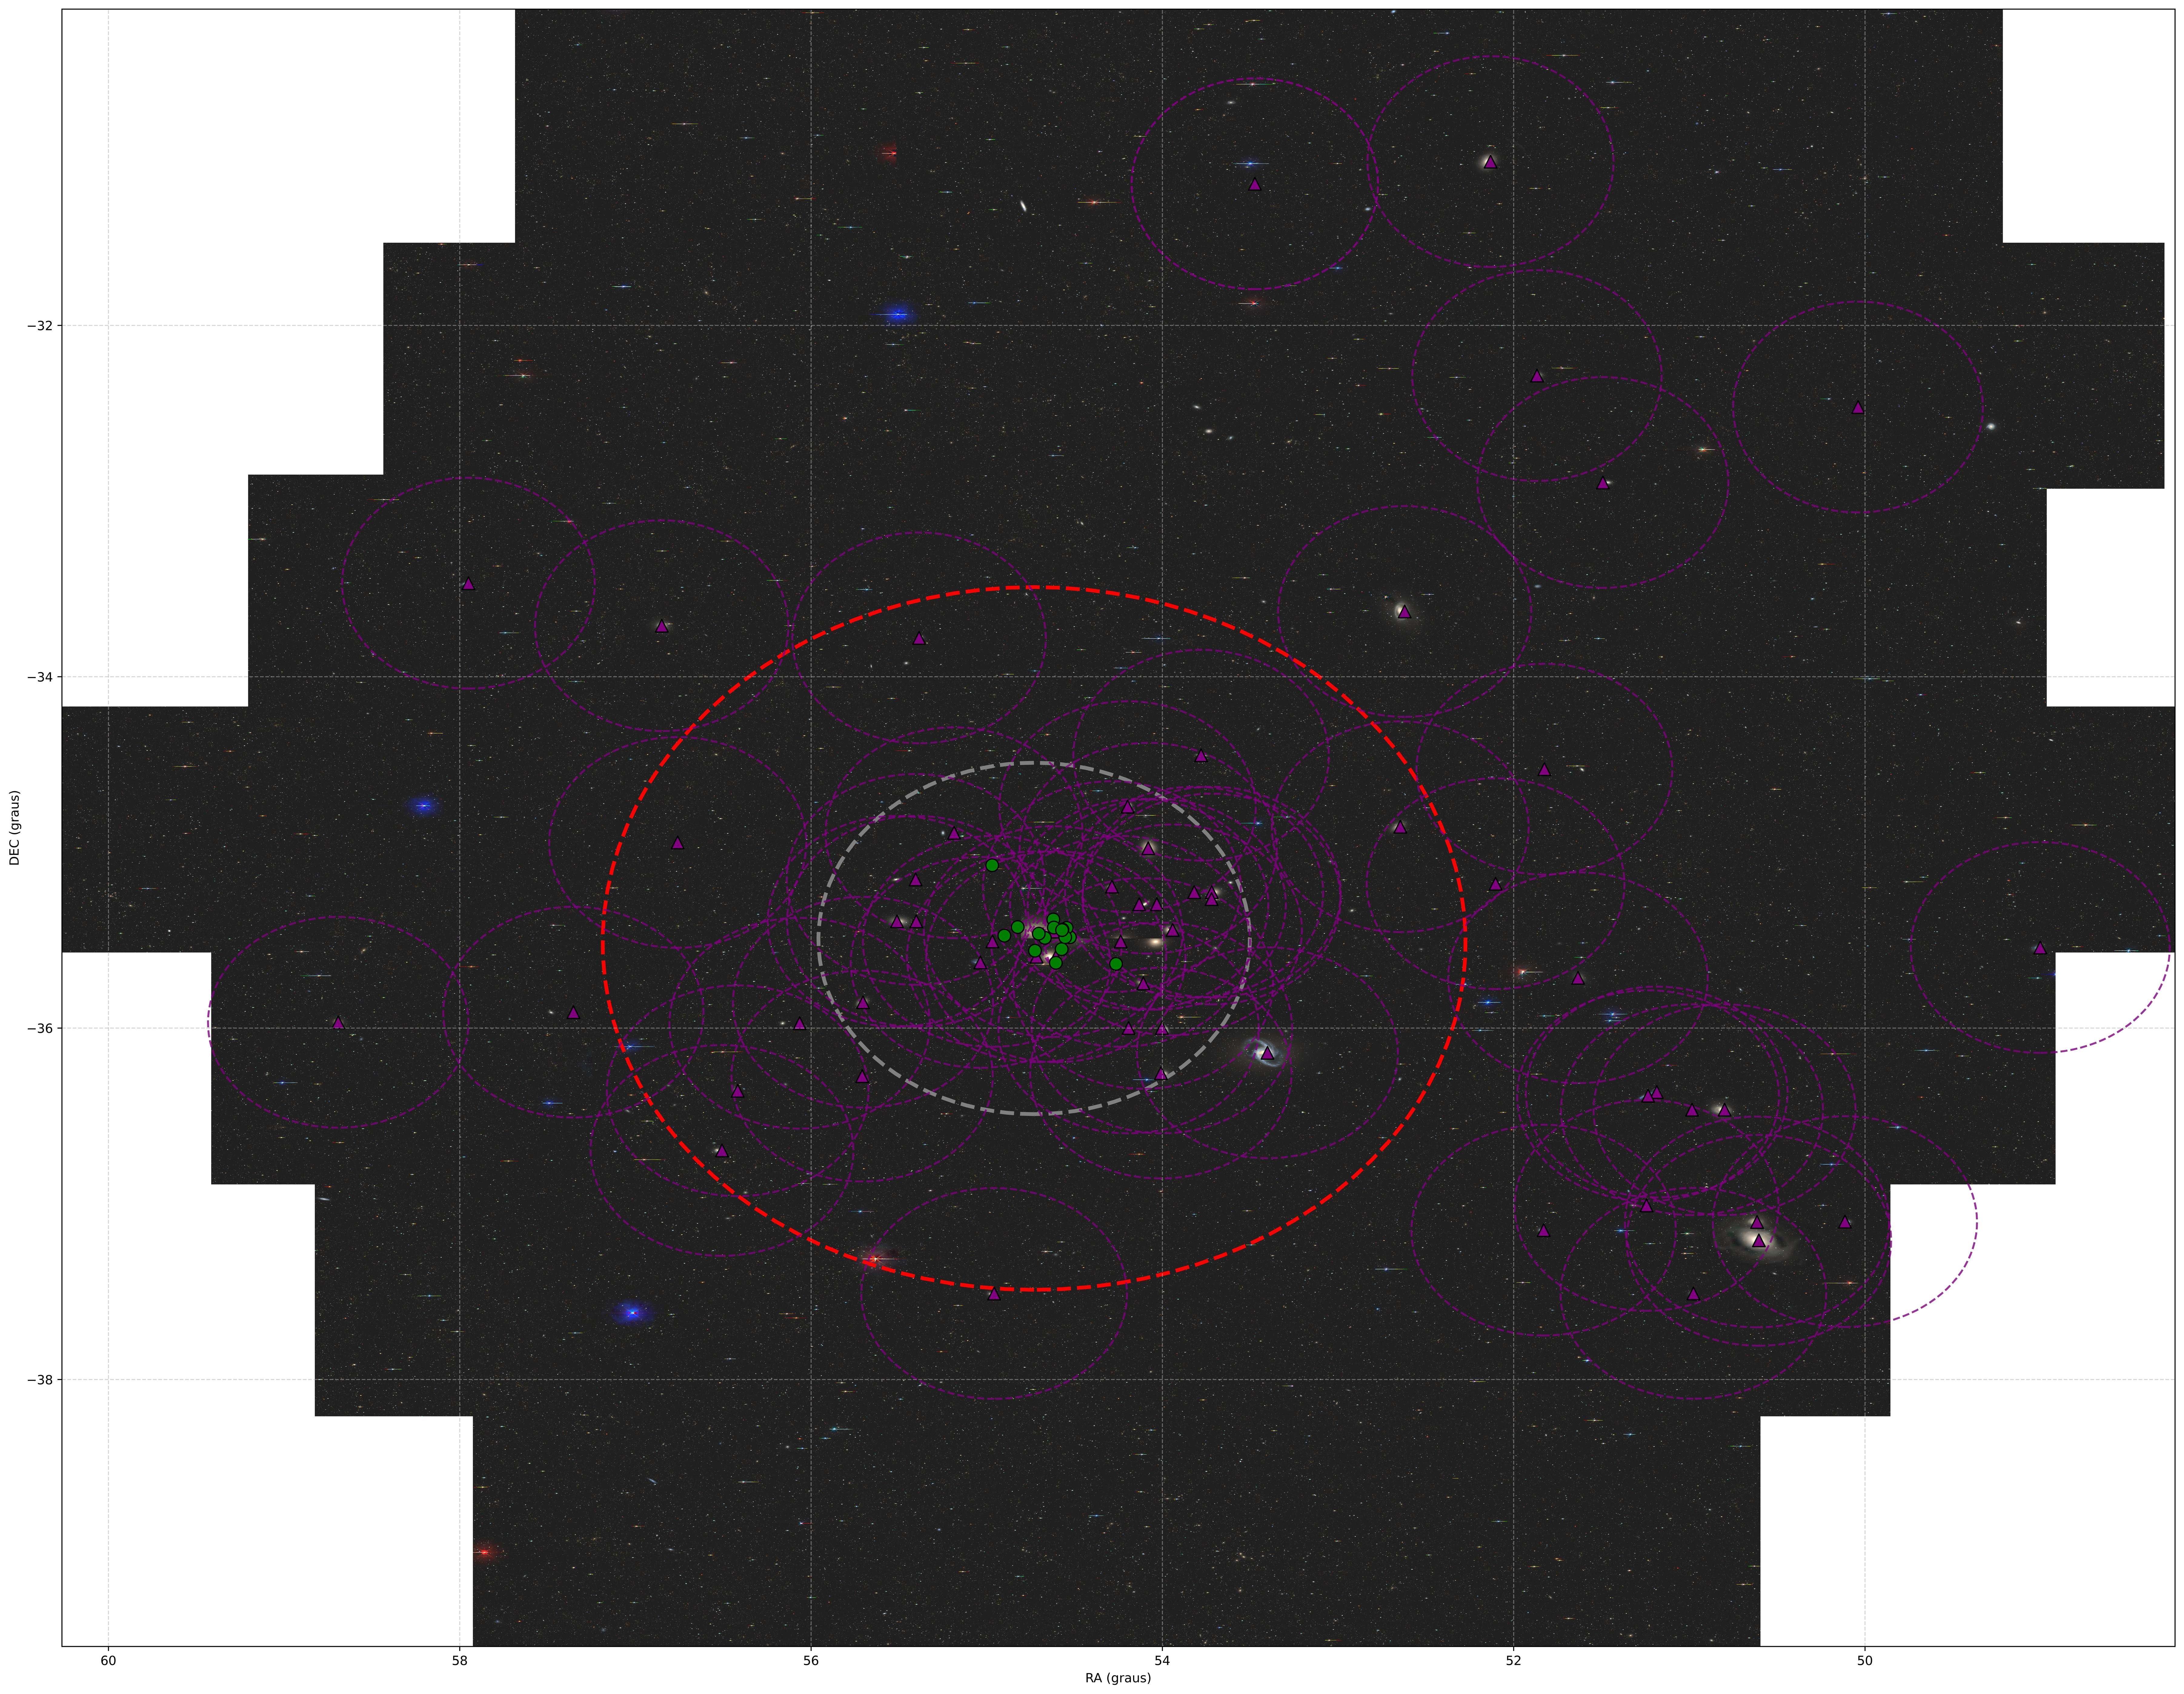
\includegraphics[width=1.\columnwidth,angle=0]{fields_fornax_center_migue_compress.jpg}
%     \caption[]{Distribuição das galáxias massivas em Fornax nos dados do S-PLUS. Os pontos em roxo representam as galáxias massivas, com um círculo indicando um raio de 200 kpc ao redor de cada uma. O arco preto corresponde ao raio de virial de Fornax, estimado em 700 kpc, enquanto o arco cinza representa o raio do núcleo (core radius), definido como 349 kpc. Ao fundo temos a imagem real do aglomerado de Fornax, criada com as imagens do Legacy Survey.}
%     \label{distribuicao_galaxias_massivas_real}
% \end{figure}

\begin{figure}[!ht]
    \centering
    \captionsetup{justification=centering}
    \begin{subfigure}[b]{0.75\textwidth}
        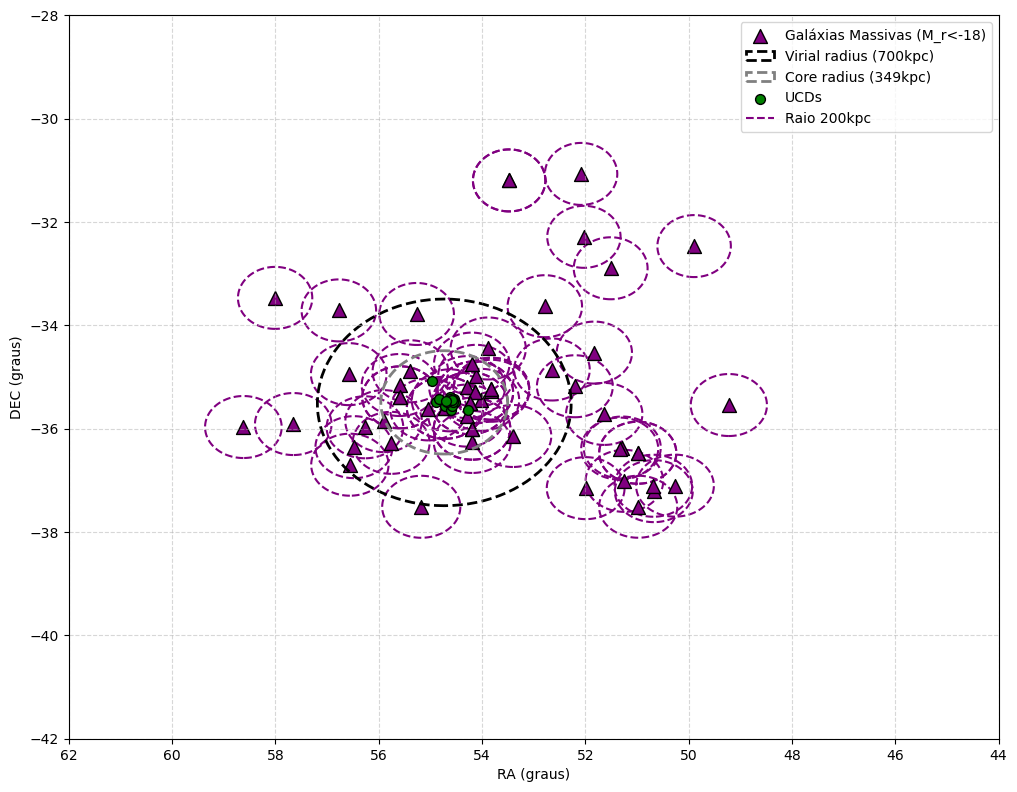
\includegraphics[width=\textwidth]{distribuicao_galaxias_massivas.png}
        \caption{}
    \end{subfigure}
    \begin{subfigure}[b]{0.75\textwidth}
        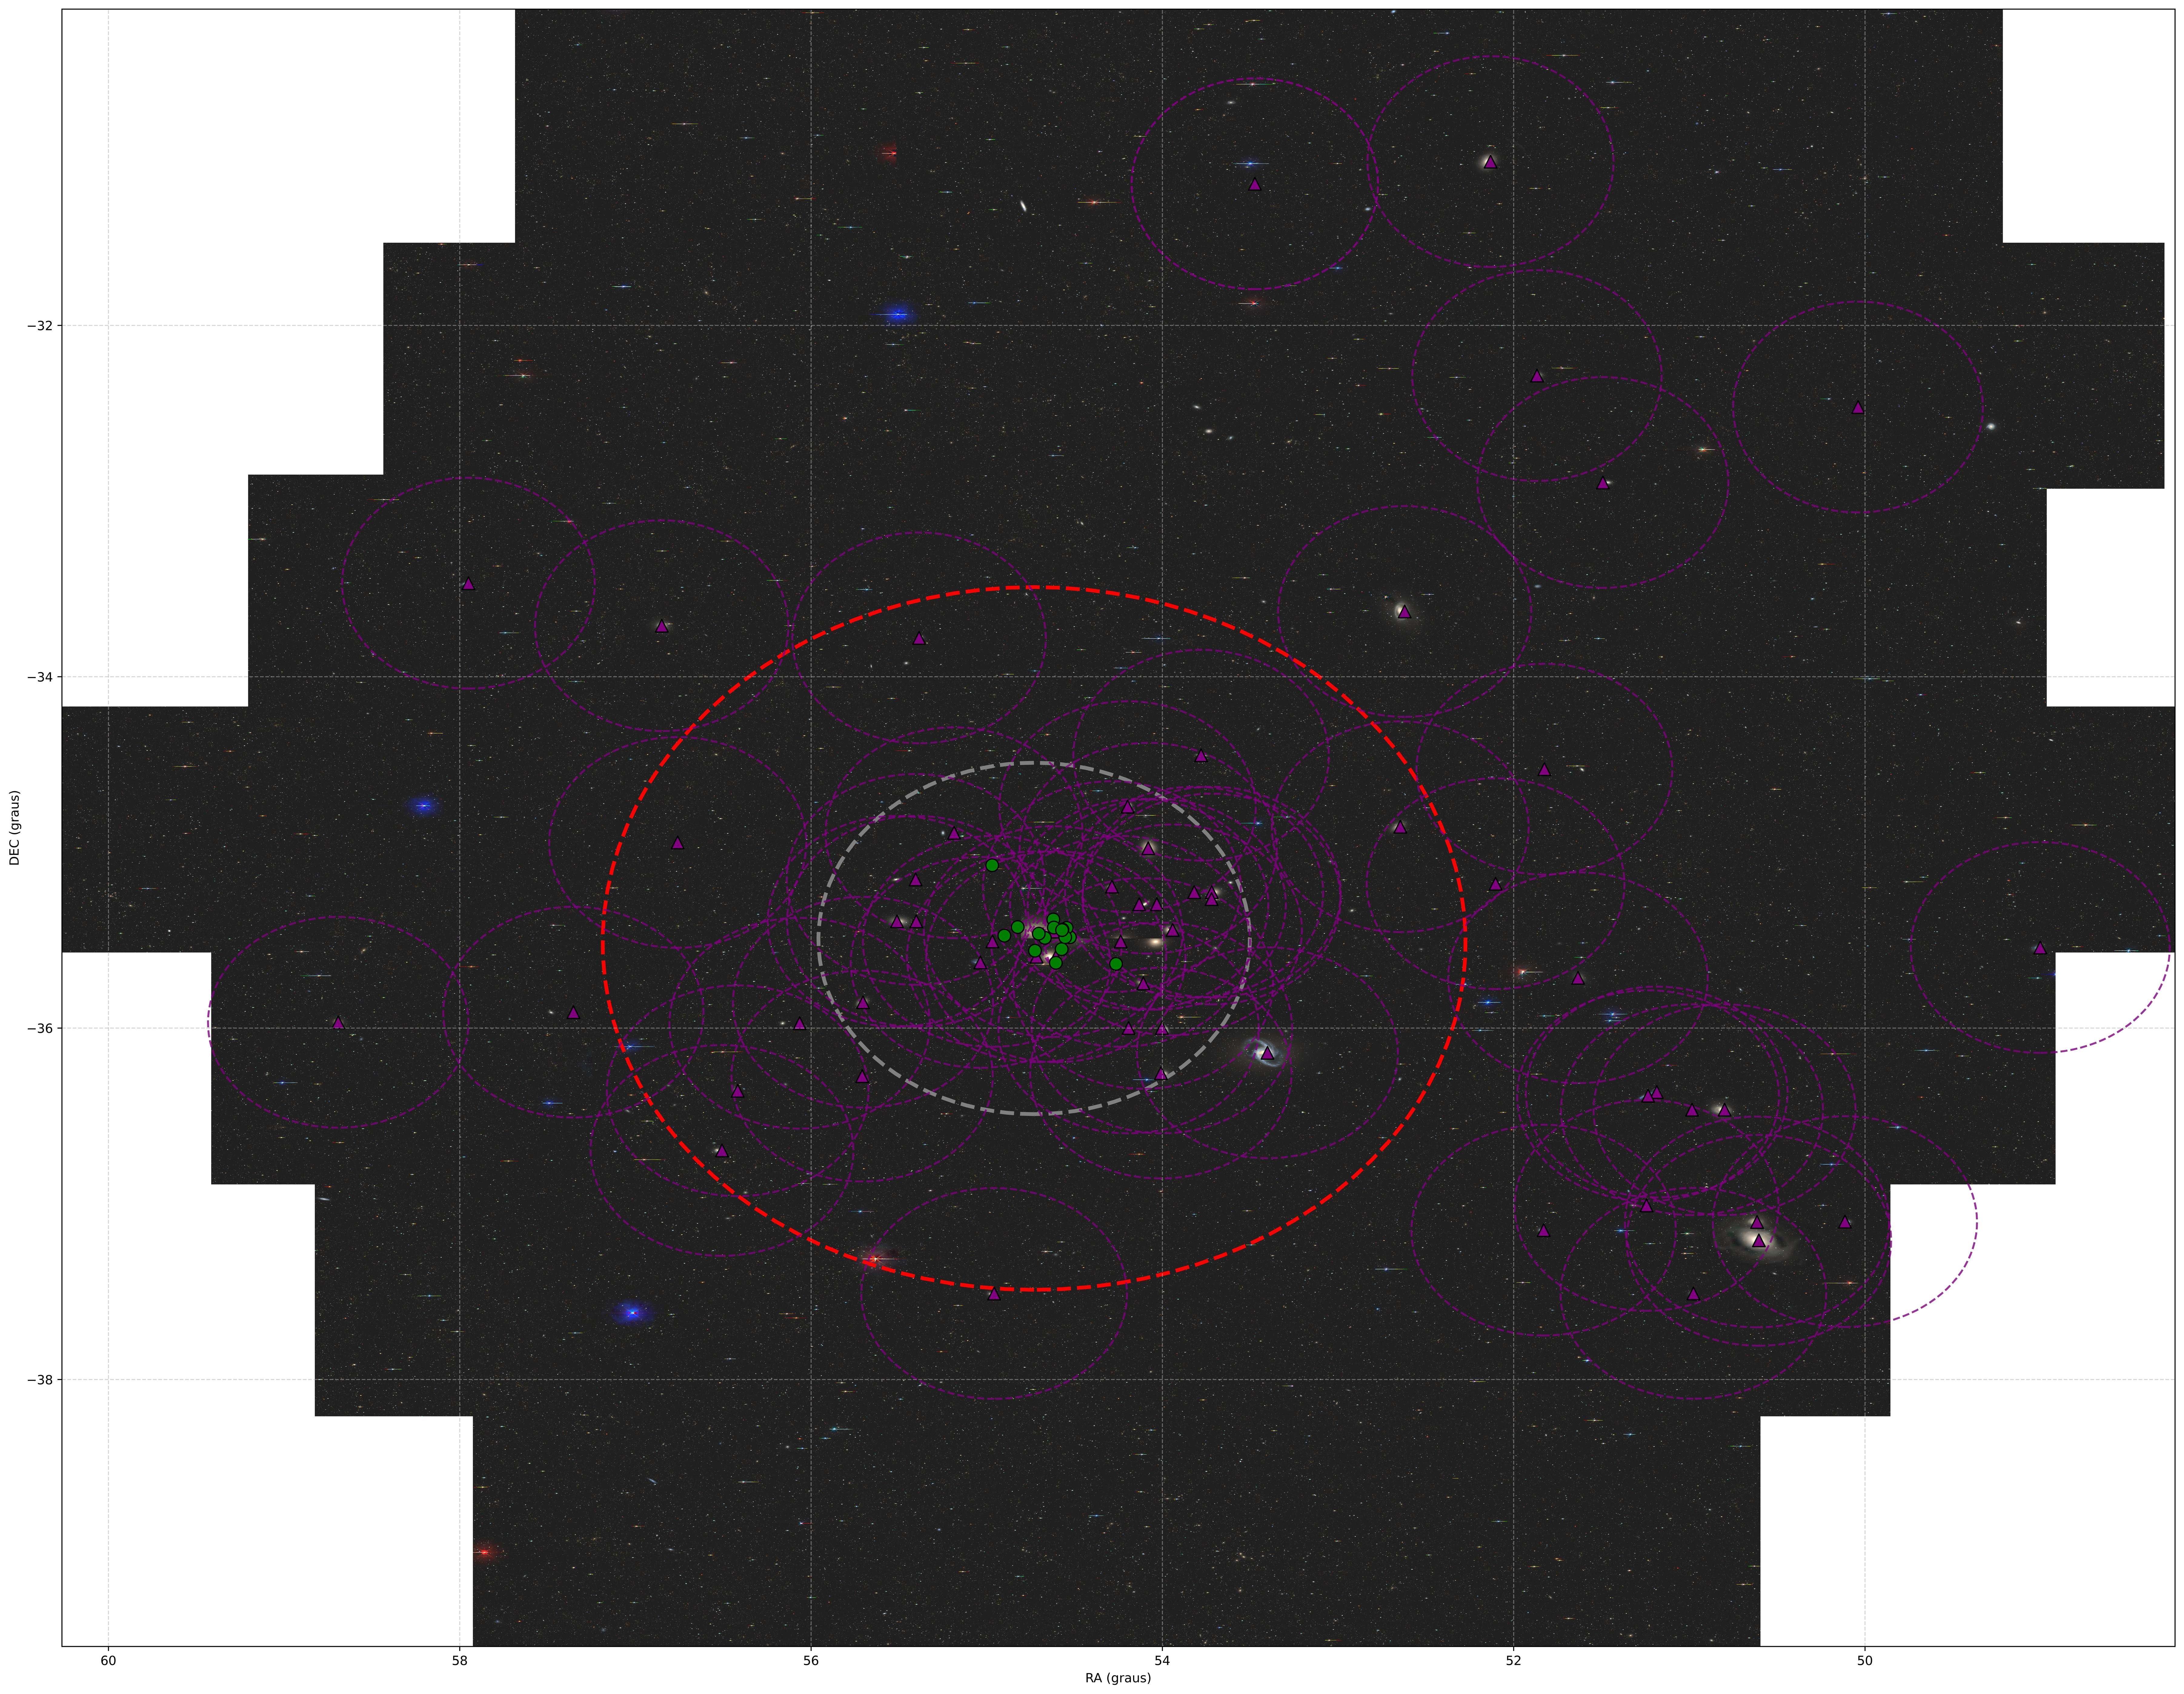
\includegraphics[width=\textwidth]{fields_fornax_center_migue_compress.jpg}
        \caption{}
    \end{subfigure}
    \caption{(a) Distribuição das galáxias massivas em Fornax nos dados do S-PLUS. Pontos em verde são as UCDs. Os pontos em roxo representam as galáxias massivas, com um círculo indicando um raio de 200 kpc ao redor de cada uma. O arco preto corresponde ao raio de virial de Fornax, estimado em 700 kpc, enquanto o arco cinza representa o raio do núcleo (core radius), definido como 349 kpc.\\ (b) Mesma imagem com a adição ao fundo da imagem real do aglomerado de Fornax, criada com as imagens do Legacy Survey.}
    \label{distribuicao_galaxias_massivas}
\end{figure}

Selecionamos, portanto, as principais galáxias massivas do aglomerado de Fornax, definidas como aquelas com magnitudes absolutas $M_r \leq -18$. As UCDs são frequentemente associadas a processos de interação gravitacional, seja em aglomerados de galáxias ou em interações com galáxias massivas. Dessa forma, a presença e a distribuição dessas galáxias massivas podem desempenhar um papel crucial na formação e localização das UCDs no aglomerado. Utilizaremos a distribuição espacial das galáxias massivas para realizar uma análise comparativa com a distribuição das candidatas a UCDs.

\section{Aprendizado de Máquina}\label{sec:aprendizado_maquina}
Neste trabalho, utilizamos aprendizado de máquina para auxiliar na identificação de candidatas a galáxias ultracompactas (UCDs) no aglomerado de Fornax, com base em dados fotométricos do S-PLUS. A distinção entre UCDs e outros objetos compactos, como estrelas, é desafiadora. Para abordar essa dificuldade, empregamos um método supervisionado que classifica os objetos em duas categorias principais com base exclusivamente na fotometria: compactos e extensos. Essa abordagem permite identificar objetos compactos com características fotométricas semelhantes às de galáxias, facilitando a seleção de candidatas a UCDs.

O processo é dividido em duas etapas principais. Primeiro, classificamos os objetos em duas categorias: compactos e extensos, com base exclusivamente na largura à meia altura (\textit{FWHM}). Objetos compactos, como estrelas e UCDs, possuem valores menores de \textit{FWHM}, enquanto objetos extensos, como galáxias, apresentam valores maiores. Essa classificação inicial é feita para separar os objetos com base em sua morfologia.

Na segunda etapa, utilizamos um classificador supervisionado treinado exclusivamente com os dados fotométricos dos objetos. Como a imensa maioria dos objetos extensos são galáxias e a maioria dos objetos compactos são estrelas, o objetivo do classificador é identificar, dentro do grupo de objetos compactos, aqueles que possuem características fotométricas semelhantes às de galáxias extensas. Esses objetos compactos, classificados como extensos pelo modelo, são então considerados candidatos a UCDs.

Em resumo, a proposta consiste em explorar a morfologia dos objetos para separá-los em compactos e extensos e, em seguida, utilizar a fotometria para identificar candidatos a UCDs entre os objetos compactos. Nas subseções seguintes, detalharemos o processo de construção da amostra de treino, o tratamento de valores faltantes, o treinamento do modelo e a avaliação do desempenho do classificador.



\subsection{Amostra de treino}\label{subsec:amostra_treino}
Para a amostra de treino, é desejável implementar uma estratégia que auxilie na identificação de candidatas a UCDs. Uma abordagem comum é a utilização de um classificador, onde um modelo é treinado com um conjunto de dados rotulados e, posteriormente, é capaz de classificar novos objetos com base nas características aprendidas durante o treinamento.

Um exemplo semelhante é o problema de classificação de quasares, que são fontes pontuais facilmente confundidas com estrelas, mas possuem características que os distinguem destas. Nesse caso, um modelo de classificação pode ser treinado com dados de quasares e estrelas, realizando a separação entre eles. No entanto, para UCDs, temos uma quantidade limitada de objetos conhecidos, impossibilitando um conjunto de dados grande o suficiente para treinar um modelo de classificação direta de UCDs.

Usamos a \textit{FWHM} normalizada para cada uma das bandas. O valor normalizado é dado pela \textit{FWHM} do objeto dividido pela \textit{FWHM} do campo. A normalização é feita para garantir que a largura do perfil de intensidade seja independente da qualidade da imagem e da região observada, quando comparada entre objetos de diferentes campos.

As estrelas, por sua natureza, são fontes pontuais; por isso, esperamos que a \textit{FWHM} desses objetos seja menor do que a de objetos extensos, como as galáxias, exceto, claro, para galáxias ultra compactas.

Realizamos um cruzamento de dados de treinamento com o catálogo GAIA DR3 \citep{GAIA_DR3}, que fornece informações de classificação estrela-galáxia-quasar. Com esses dados, selecionamos um subconjunto de objetos com as probabilidades de serem estrelas e galáxias maiores que 90\%. A partir desse subconjunto, analisamos a distribuição dos valores de \textit{FWHM} para estrelas e galáxias em cada banda fotométrica.

Na Figura \ref{distribution_of_stars_and_galaxies}, apresentamos um histograma da distribuição de \textit{FWHM} para estrelas e galáxias na banda $r$. Optamos por utilizar a banda $r$ como referência devido à sua maior profundidade, além de observarmos que, em comparação com outras bandas, os picos de \textit{FWHM} para estrelas e galáxias estão mais bem separados, facilitando a distinção entre as duas classes. A Figura \ref{distribution_of_stars_and_galaxies_u} monstra um dos outros exemplos de bandas, a banda $u$. Vemos que a separação entre as duas classes não é tão clara quanto na banda $r$, e o mesmo ocorre para as outras bandas. Portanto, a banda $r$ é a mais adequada para o nosso estudo. 


\begin{center}
    \begin{minipage}{0.45\textwidth}
        \centering
        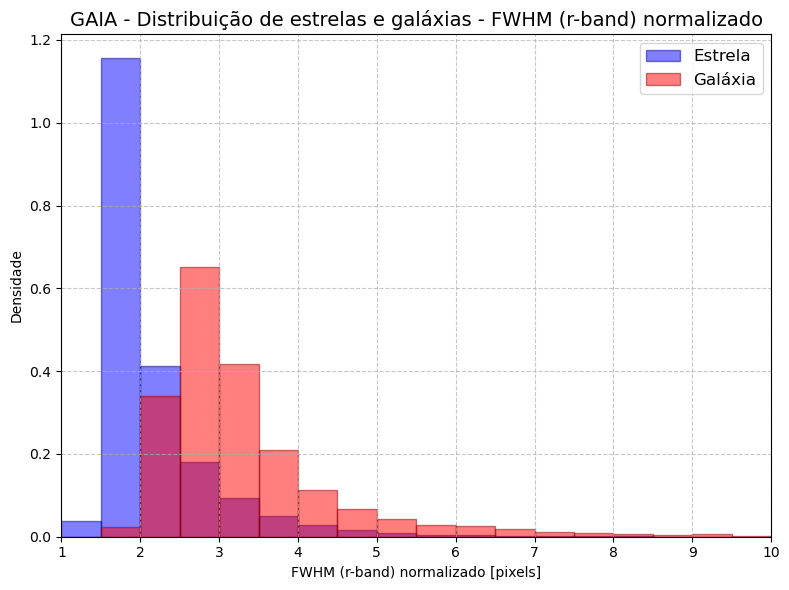
\includegraphics[width=\linewidth]{distribution_of_stars_and_galaxies.png}
        \captionsetup{}
        \captionof{figure}{Histograma da distribuição de \textit{FWHM (r-band) normalizado} dos objetos do cruzamento do S-PLUS DR4 de Fornax, com o catálogo GAIA DR3 com a classificação para estrelas e galáxias com probabilidade maior que 90\%.}  
        \label{distribution_of_stars_and_galaxies}
    \end{minipage}
    \hfill
    \begin{minipage}{0.45\textwidth}
        \centering
        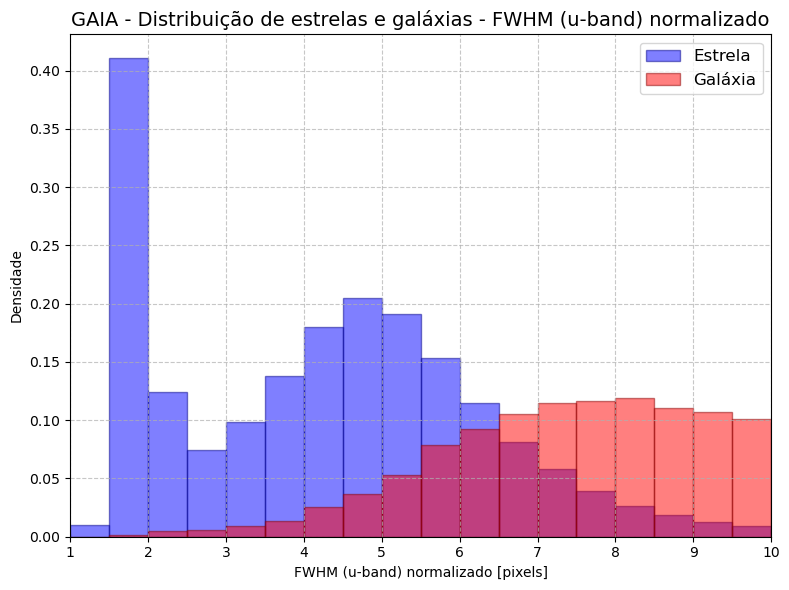
\includegraphics[width=\linewidth]{distribution_of_stars_and_galaxies_u.png}
        \captionsetup{}
        \captionof{figure}{Histograma da distribuição de \textit{FWHM (u-band) normalizado} dos objetos do cruzamento do S-PLUS DR4 de Fornax, com o catálogo GAIA DR3 com a classificação para estrelas e galáxias com probabilidade maior que 90\%.}
        \label{distribution_of_stars_and_galaxies_u}
    \end{minipage}
\end{center}

Há uma diferença entre os picos das distribuições de \textit{FWHM} para estrelas e galáxias. Portanto, o objetivo é definir um corte na \textit{FWHM} para selecionar dois conjuntos: um contendo objetos compactos e outro contendo objetos extensos. No conjunto de objetos compactos, predominam as estrelas, enquanto no conjunto de objetos extensos, as galáxias são mais representativas.

A hipótese é que o modelo aprenda a distinguir as propriedades fotométricas de estrelas e galáxias independentemente da morfologia (ou FWHM) do objeto; numa segunda etapa, procuramos entre os objetos com morfologia estelar aqueles cuja fotometria indica que têm alta probabilidade de serem galáxias.

É importante destacar que, além das galáxias compactas, existem estrelas que possuem espectros muito semelhantes aos das galáxias, especialmente em regiões de baixa resolução espectral ou em levantamentos fotométricos. Essas estrelas podem ser confundidas com galáxias, levando também a uma contaminação na amostra de galáxias.

Para identificar, na Figura \ref{distribution_of_stars_and_galaxies}, a melhor divisão entre as duas classes, estabelecemos alguns cortes em \textit{FWHMn} visando encontrar aquele que melhor separa cada população, minimizando a contaminação entre as duas populações. Para cada corte, definimos duas variáveis: Pureza e Completeza, ambas com respeito às galáxias (estas quantidades estão definidas mais formalmente na seção \ref{subsec:analise_modelo}). A Pureza representa a fração de galáxias após o corte em relação ao total de objetos restantes no corte final, fornecendo uma medida da pureza das galáxias no subconjunto. A Pureza é uma métrica que indica a proporção de galáxias corretamente identificadas em relação ao total de objetos classificados como galáxias. Ela também é conhecida como precisão, sendo sua definição dada na equação \ref{eq:precisao}.

Por outro lado, a Completeza representa a fração de galáxias após o corte em relação ao número total de galáxias que existiam, fornecendo uma estimativa de quantas galáxias são perdidas durante a seleção. Ela é definida na equação \ref{eq:completeza}.

A Figura \ref{purity_completeness} ilustra as métricas de Pureza e Completeza, conforme definido na seção \ref{subsec:analise_modelo}. Apresentamos junto nela as curvas do produto entre Pureza e Completeza, juntamente com o F1-score. O ponto ideal para a separação das classes é identificado no valor máximo do F1-score. Esse ponto representa o corte que faremos para separação entre as duas classes.

\begin{figure}[!ht]
    \centering
    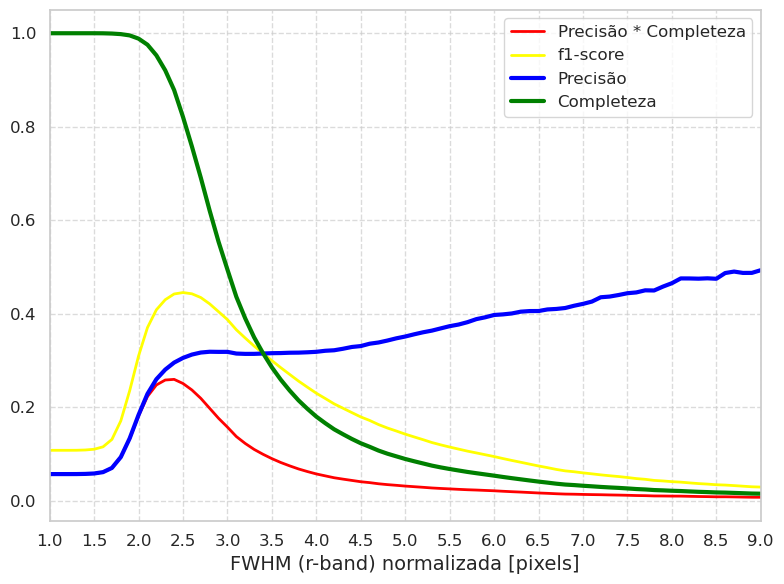
\includegraphics[width=0.95\columnwidth,angle=0]{purity_completeness.png}
    \caption[]{Relação entre Pureza, Completeza e F1-score para diferentes cortes de \textit{FWHM}. O ponto ideal para a separação das classes é identificado no valor máximo do F1-score. Esse ponto representa o corte que faremos para separação entre as duas classes.}
    \label{purity_completeness}
\end{figure}

O valor máximo selecionado para o corte corresponde a um \textit{FWHM (r-band)} de 2,5 pixels. Esse corte representa o ponto de maximização para a separação das classes, com as galáxias associadas à classe de objetos extensos. No entanto, após alguns testes, decidimos realizar um corte para objetos compactos com \textit{FWHM} menores que 2 pixels, o que apresentou melhores resultados nos classificadores iniciais testados. Assim, para a amostra de treino, os objetos com \textit{FWHM (r-band)} menores que 2 pixels são considerados compactos, enquanto os objetos com \textit{FWHM (r-band)} maiores que 2,5 pixels são considerados extensos. Os demais cortes para a seleção de objetos compactos e extensos são descritos na subseção \ref{subsec:cuts}.

Os objetos com valores de \textit{FWHM} entre 2 e 2,5 pixels são considerados de transição, ou seja, não são classificados como compactos nem extensos para a amostra de treino devido à incerteza na classificação. No entanto, esses dados ainda serão utilizados na busca por candidatas a UCDs, aplicando o modelo treinado. Assim, esses objetos de transição não são incluídos no treinamento do modelo, mas permanecem na amostra de análise.

Na Figura \ref{amostra_treino}, temos a magnitude \textit{g\_APER\_6} em função da \textit{FWHM (r-band)} para a divisão entre as duas classes adotadas.

\begin{figure}[!ht]
    \centering
    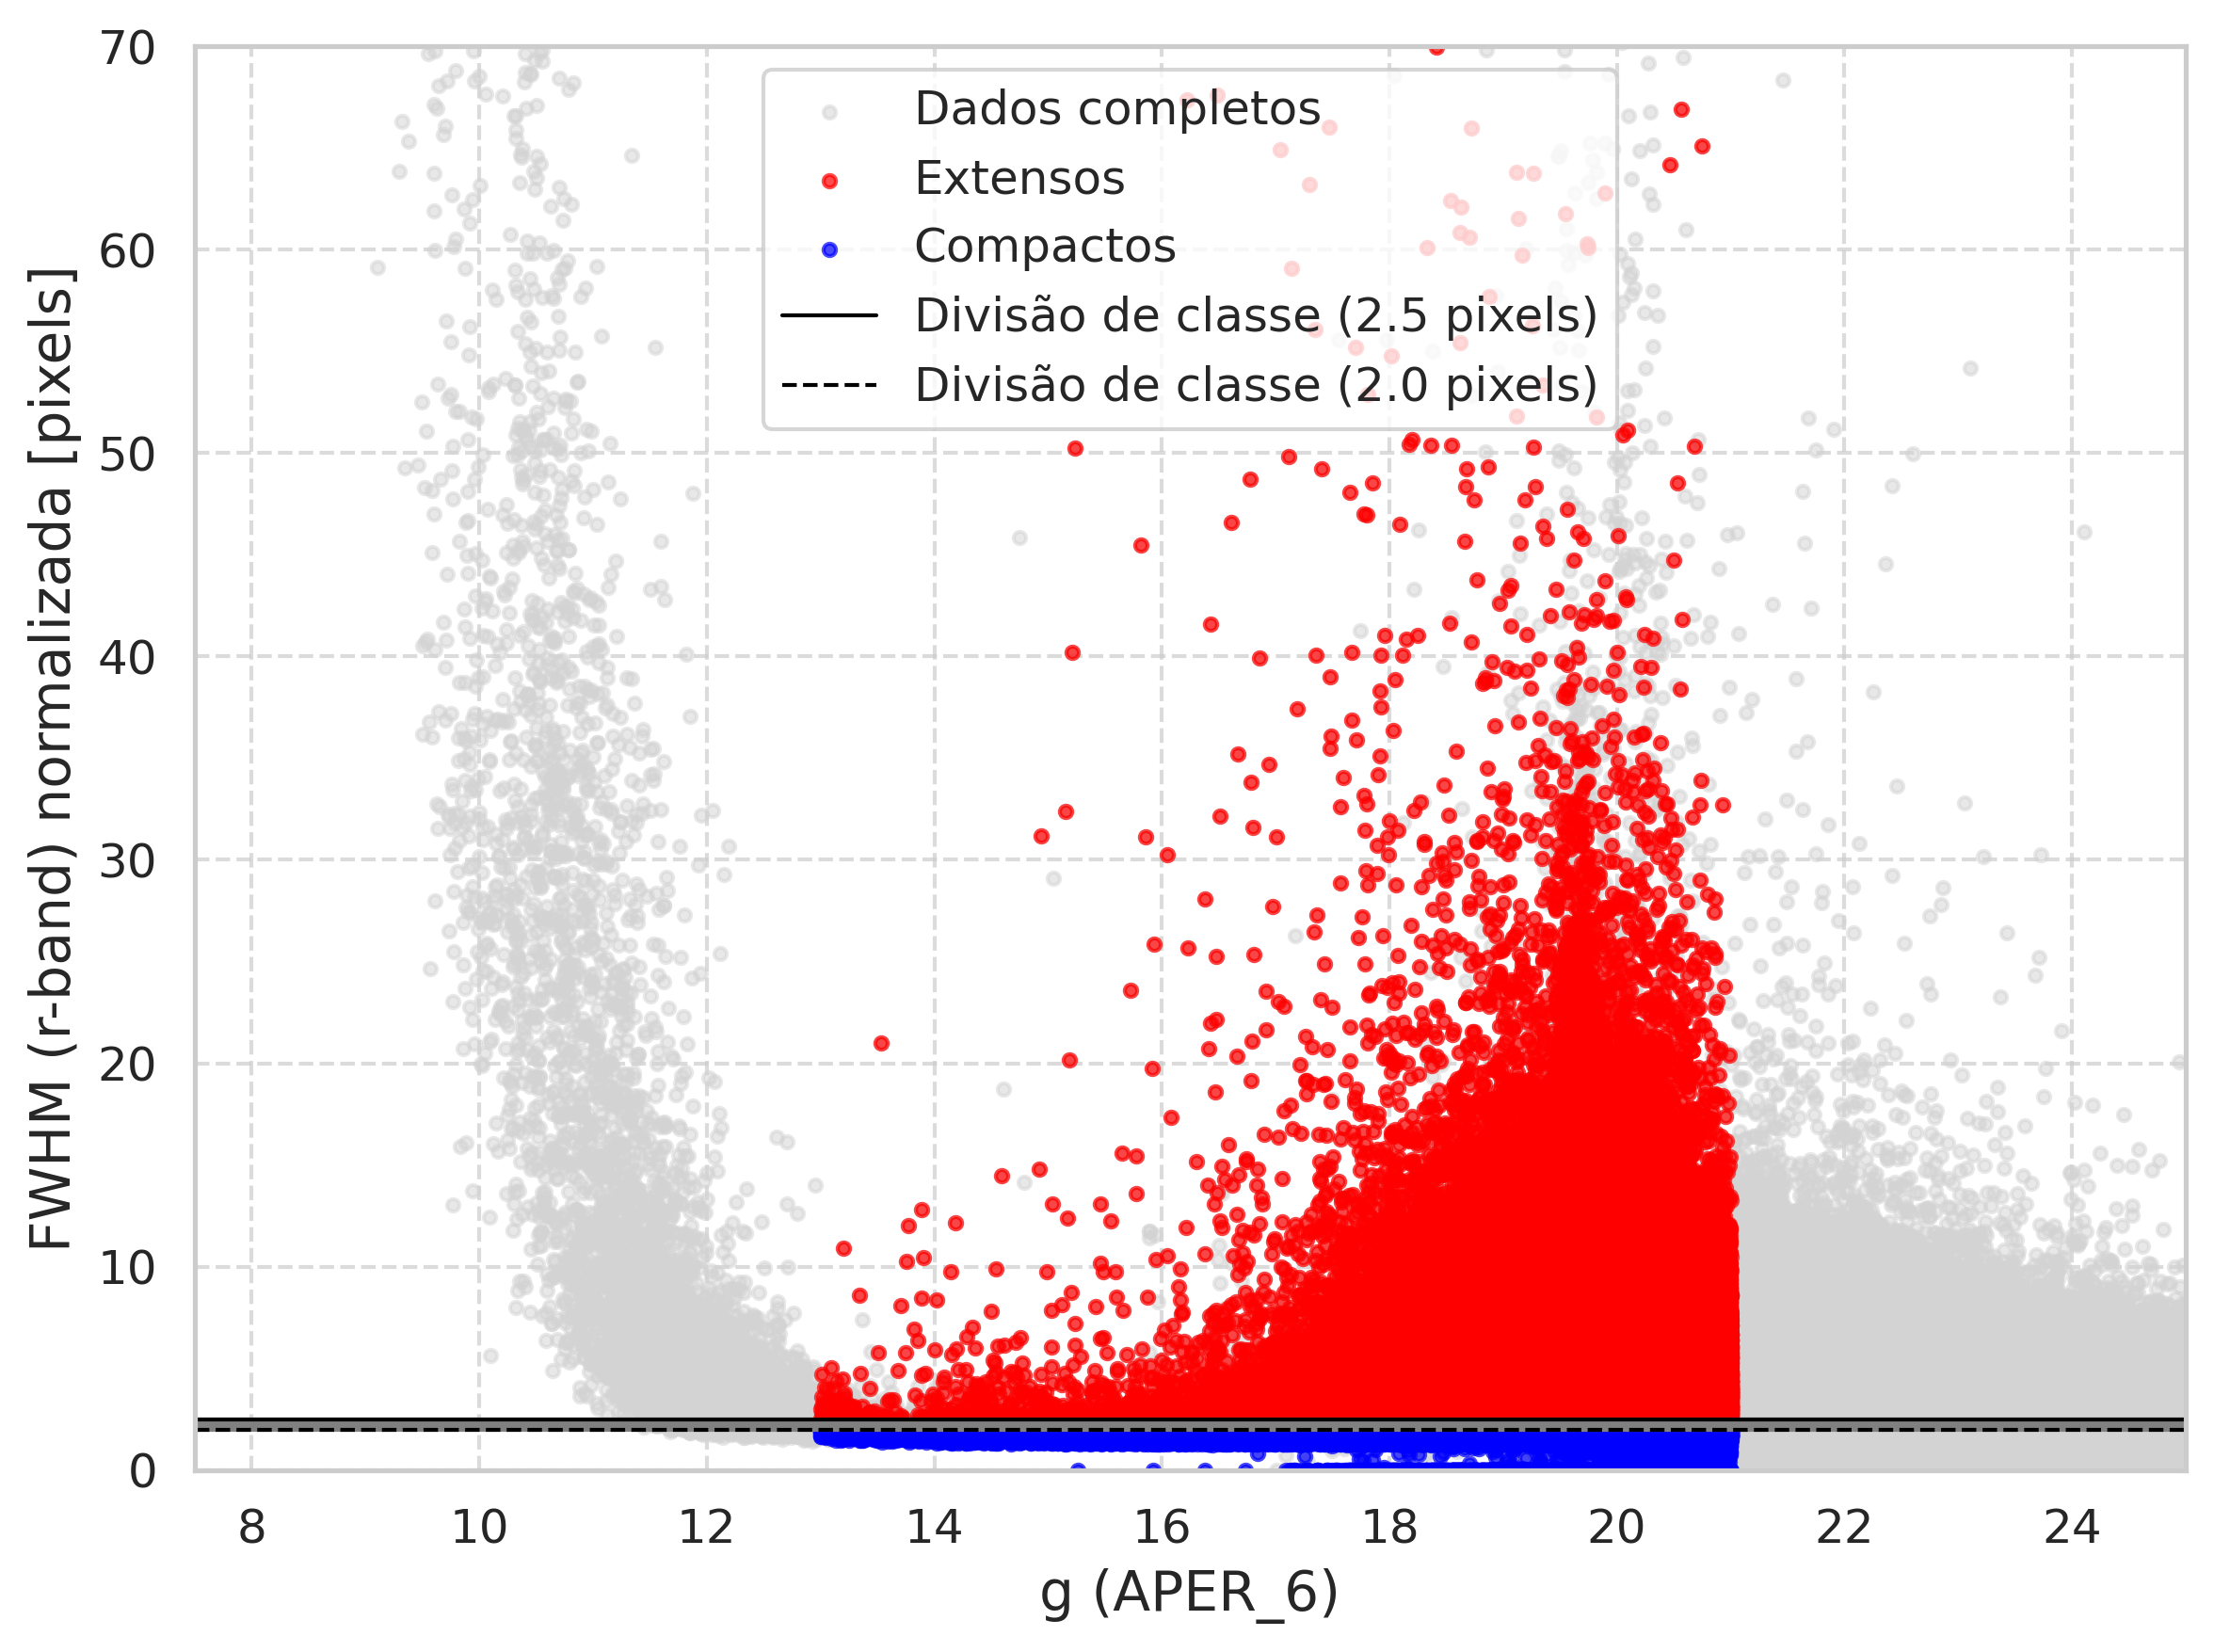
\includegraphics[width=0.85\columnwidth,angle=0]{amostra_treino.png}
    \caption[]{Distribuição da Largura Total na Metade Máxima (\textit{FWHM} r-band) em função da magnitude \textit{g\_APER\_6} para objetos na região de Fornax, usando dados do S-PLUS Data Release 4. Objetos compactos são representados por pontos azuis, enquanto objetos extensos são indicados por pontos vermelhos. Os dados totais são mostrados em cinza. Divisão das classes: compactos (\textit{FWHM}$\leq$2 pixels) e extensos (\textit{FWHM}$\geq$2.5 pixels). Os dados entre 2 e 2.5 pixels não são usados para o treinamento do modelo, mas são mantidos na amostra de análise.}
    \label{amostra_treino}
\end{figure}

\subsection{Valores faltantes na amostra de treino}\label{subsec:valores_faltantes}
Ao preparar os dados para treinar modelos com medições do S-PLUS, decidimos alterar os valores das magnitudes na abertura APER\_6 acima de 30 para \texttt{NaN} (Not a Number). Essa decisão foi tomada para evitar que objetos com medições de baixa qualidade influenciassem o treinamento do modelo.

Na Figura \ref{missing_values_hist} temos um gráfico da fração de dados disponíveis para cada uma das bandas fotométricas.

\begin{figure}[!ht]
    \begin{center}
    % \setcaptionmargin{1cm}
    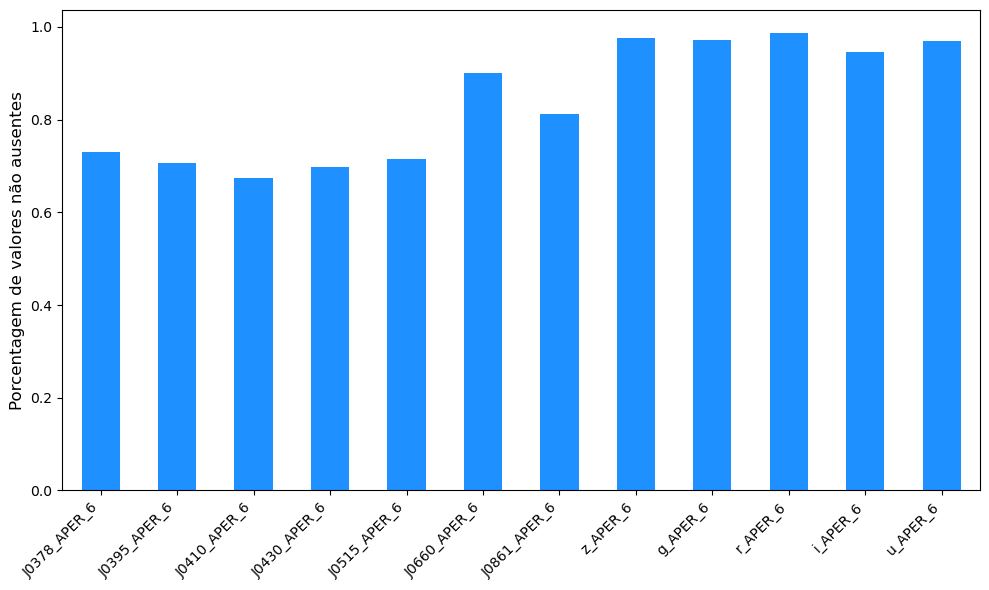
\includegraphics[width=0.8\columnwidth,angle=0]{missing_values_hist.png}
    \caption[]{Fotometria disponível em cada banda fotométrica. Cada barra representa a fração de objetos com valores disponíveis para a respectiva banda.}
    \label{missing_values_hist}
    \end{center}
\end{figure}

O gráfico mostra que a quantidade de dados ausentes varia consideravelmente entre as diferentes bandas fotométricas. A banda $u$, juntamente com algumas bandas estreitas no azul, como $J0378$, $J0395$, $J0410$ e $J0430$, apresentam a maior quantidade de valores faltantes, o que pode prejudicar a análise.

Mostramos na Figura \ref{msno_matriz} uma visualização da distribuição dos dados faltantes, onde cada linha representa um objeto e cada coluna uma banda fotométrica. As células em branco indicam valores faltantes. A Figura \ref{msno_matriz_ord} mostra a mesma matriz, mas ordenada pela primeira coluna de atributos. Ordenamos a matriz para identificar padrões de valores faltantes que possam ser úteis para a imputação dos dados.

\begin{center}
    \begin{minipage}{0.45\textwidth}
        \centering
        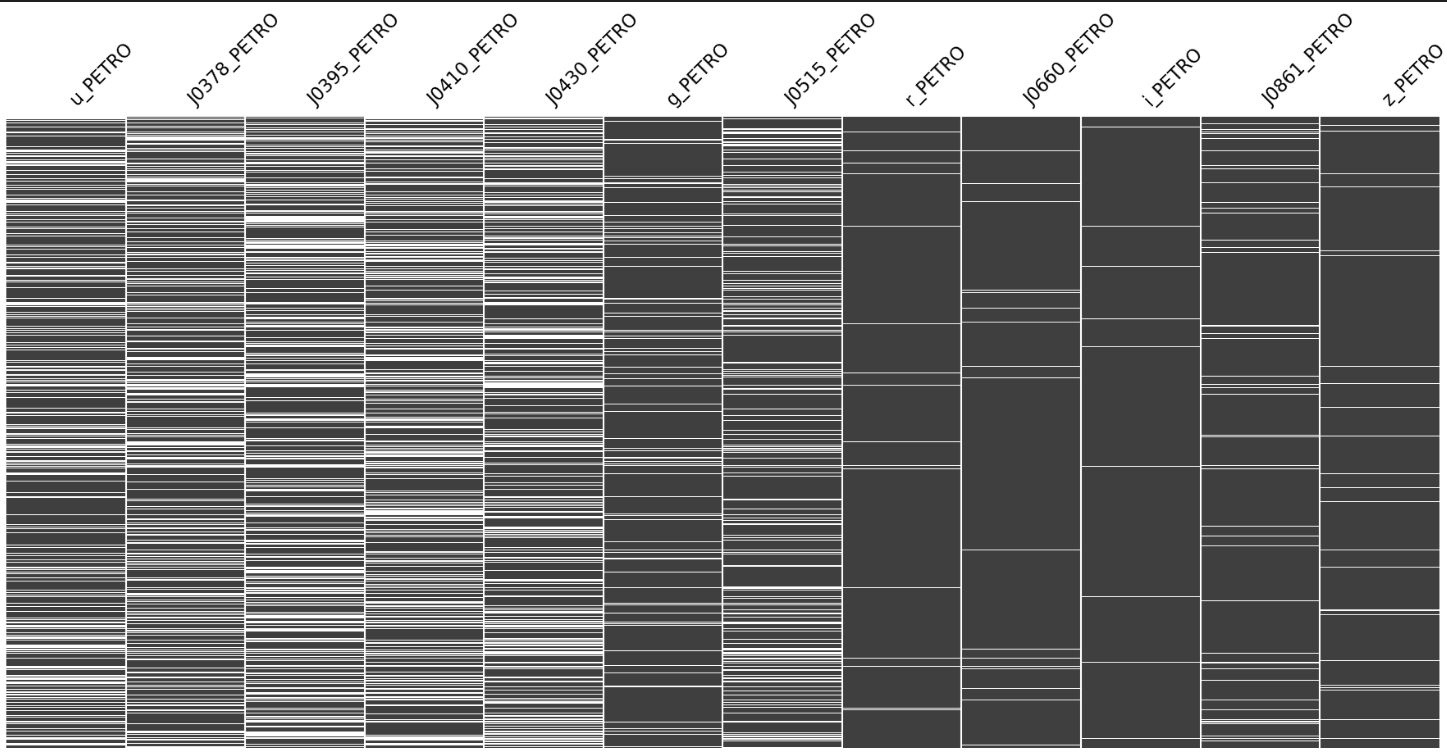
\includegraphics[width=\linewidth]{msno_matriz.png}
        \captionsetup{}
        \captionof{figure}{Distribuição de valores em cada banda fotométrica. Cada barra vertical representa as linhas da tabela original. As linhas em preto indicam objetos com valores disponíveis para a respectiva banda, enquanto os espaços em branco correspondem a linhas na tabela sem valores medidos.}
        \label{msno_matriz}
    \end{minipage}
    \hfill
    \begin{minipage}{0.45\textwidth}
        \centering
        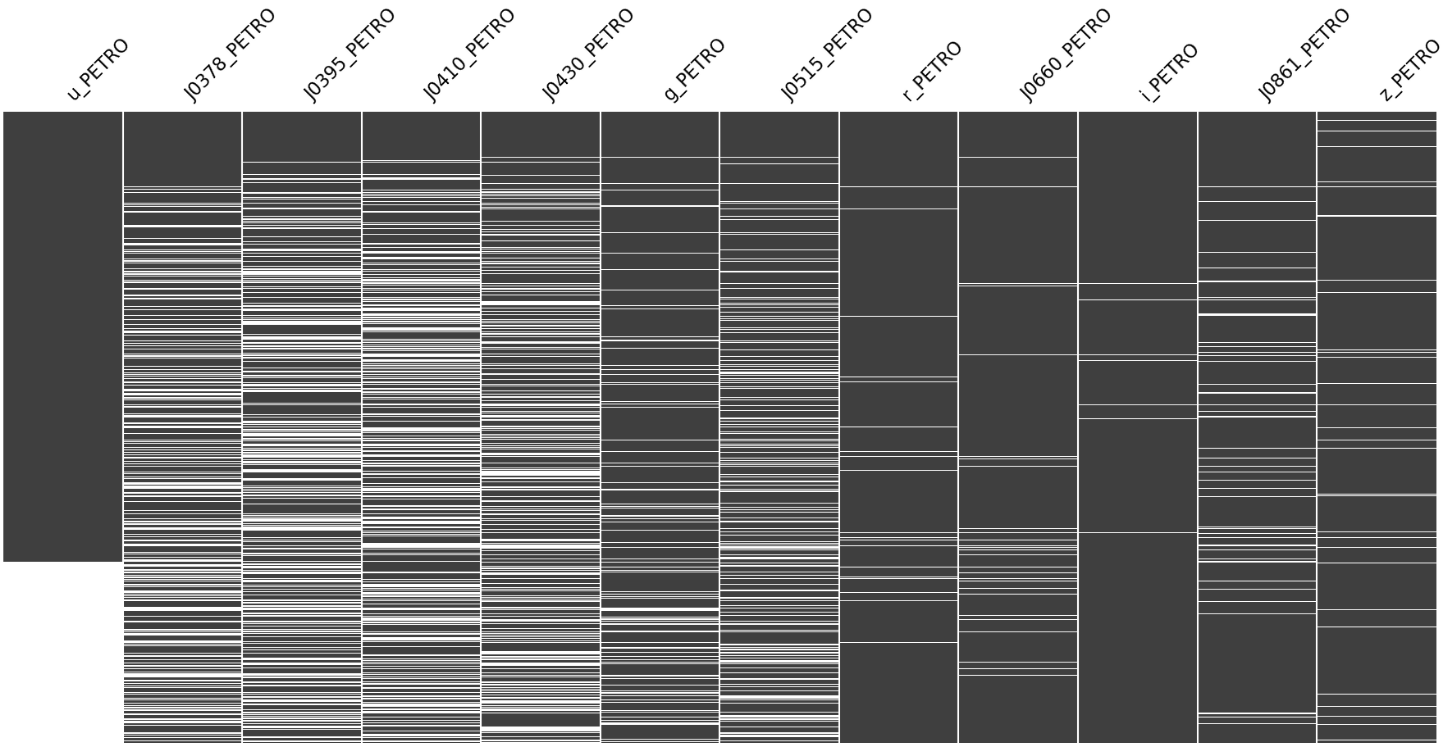
\includegraphics[width=\linewidth]{msno_matriz_ord.png}
        \captionsetup{}
        \captionof{figure}{Distribuição de valores em cada banda fotométrica, ordenada de forma que os valores disponíveis na última coluna de atributos sejam agrupados no início (coluna preenchida), enquanto os valores faltantes sejam posicionados ao final.}
        \label{msno_matriz_ord}
    \end{minipage}
\end{center}

Uma maneira melhor de visualizar se esses valores ausentes têm alguma correlação é mostrada na Figura \ref{matriz_correlacao}, que apresenta a matriz de correlação entre os valores faltantes. Valores próximos de 1 ou -1 indicam que os valores faltantes estão, respectivamente, positivamente ou negativamente correlacionados. Valores próximos de 0 indicam que os valores faltantes são independentes.

\begin{figure}[!ht]
    \begin{center}
    % \setcaptionmargin{1cm}
    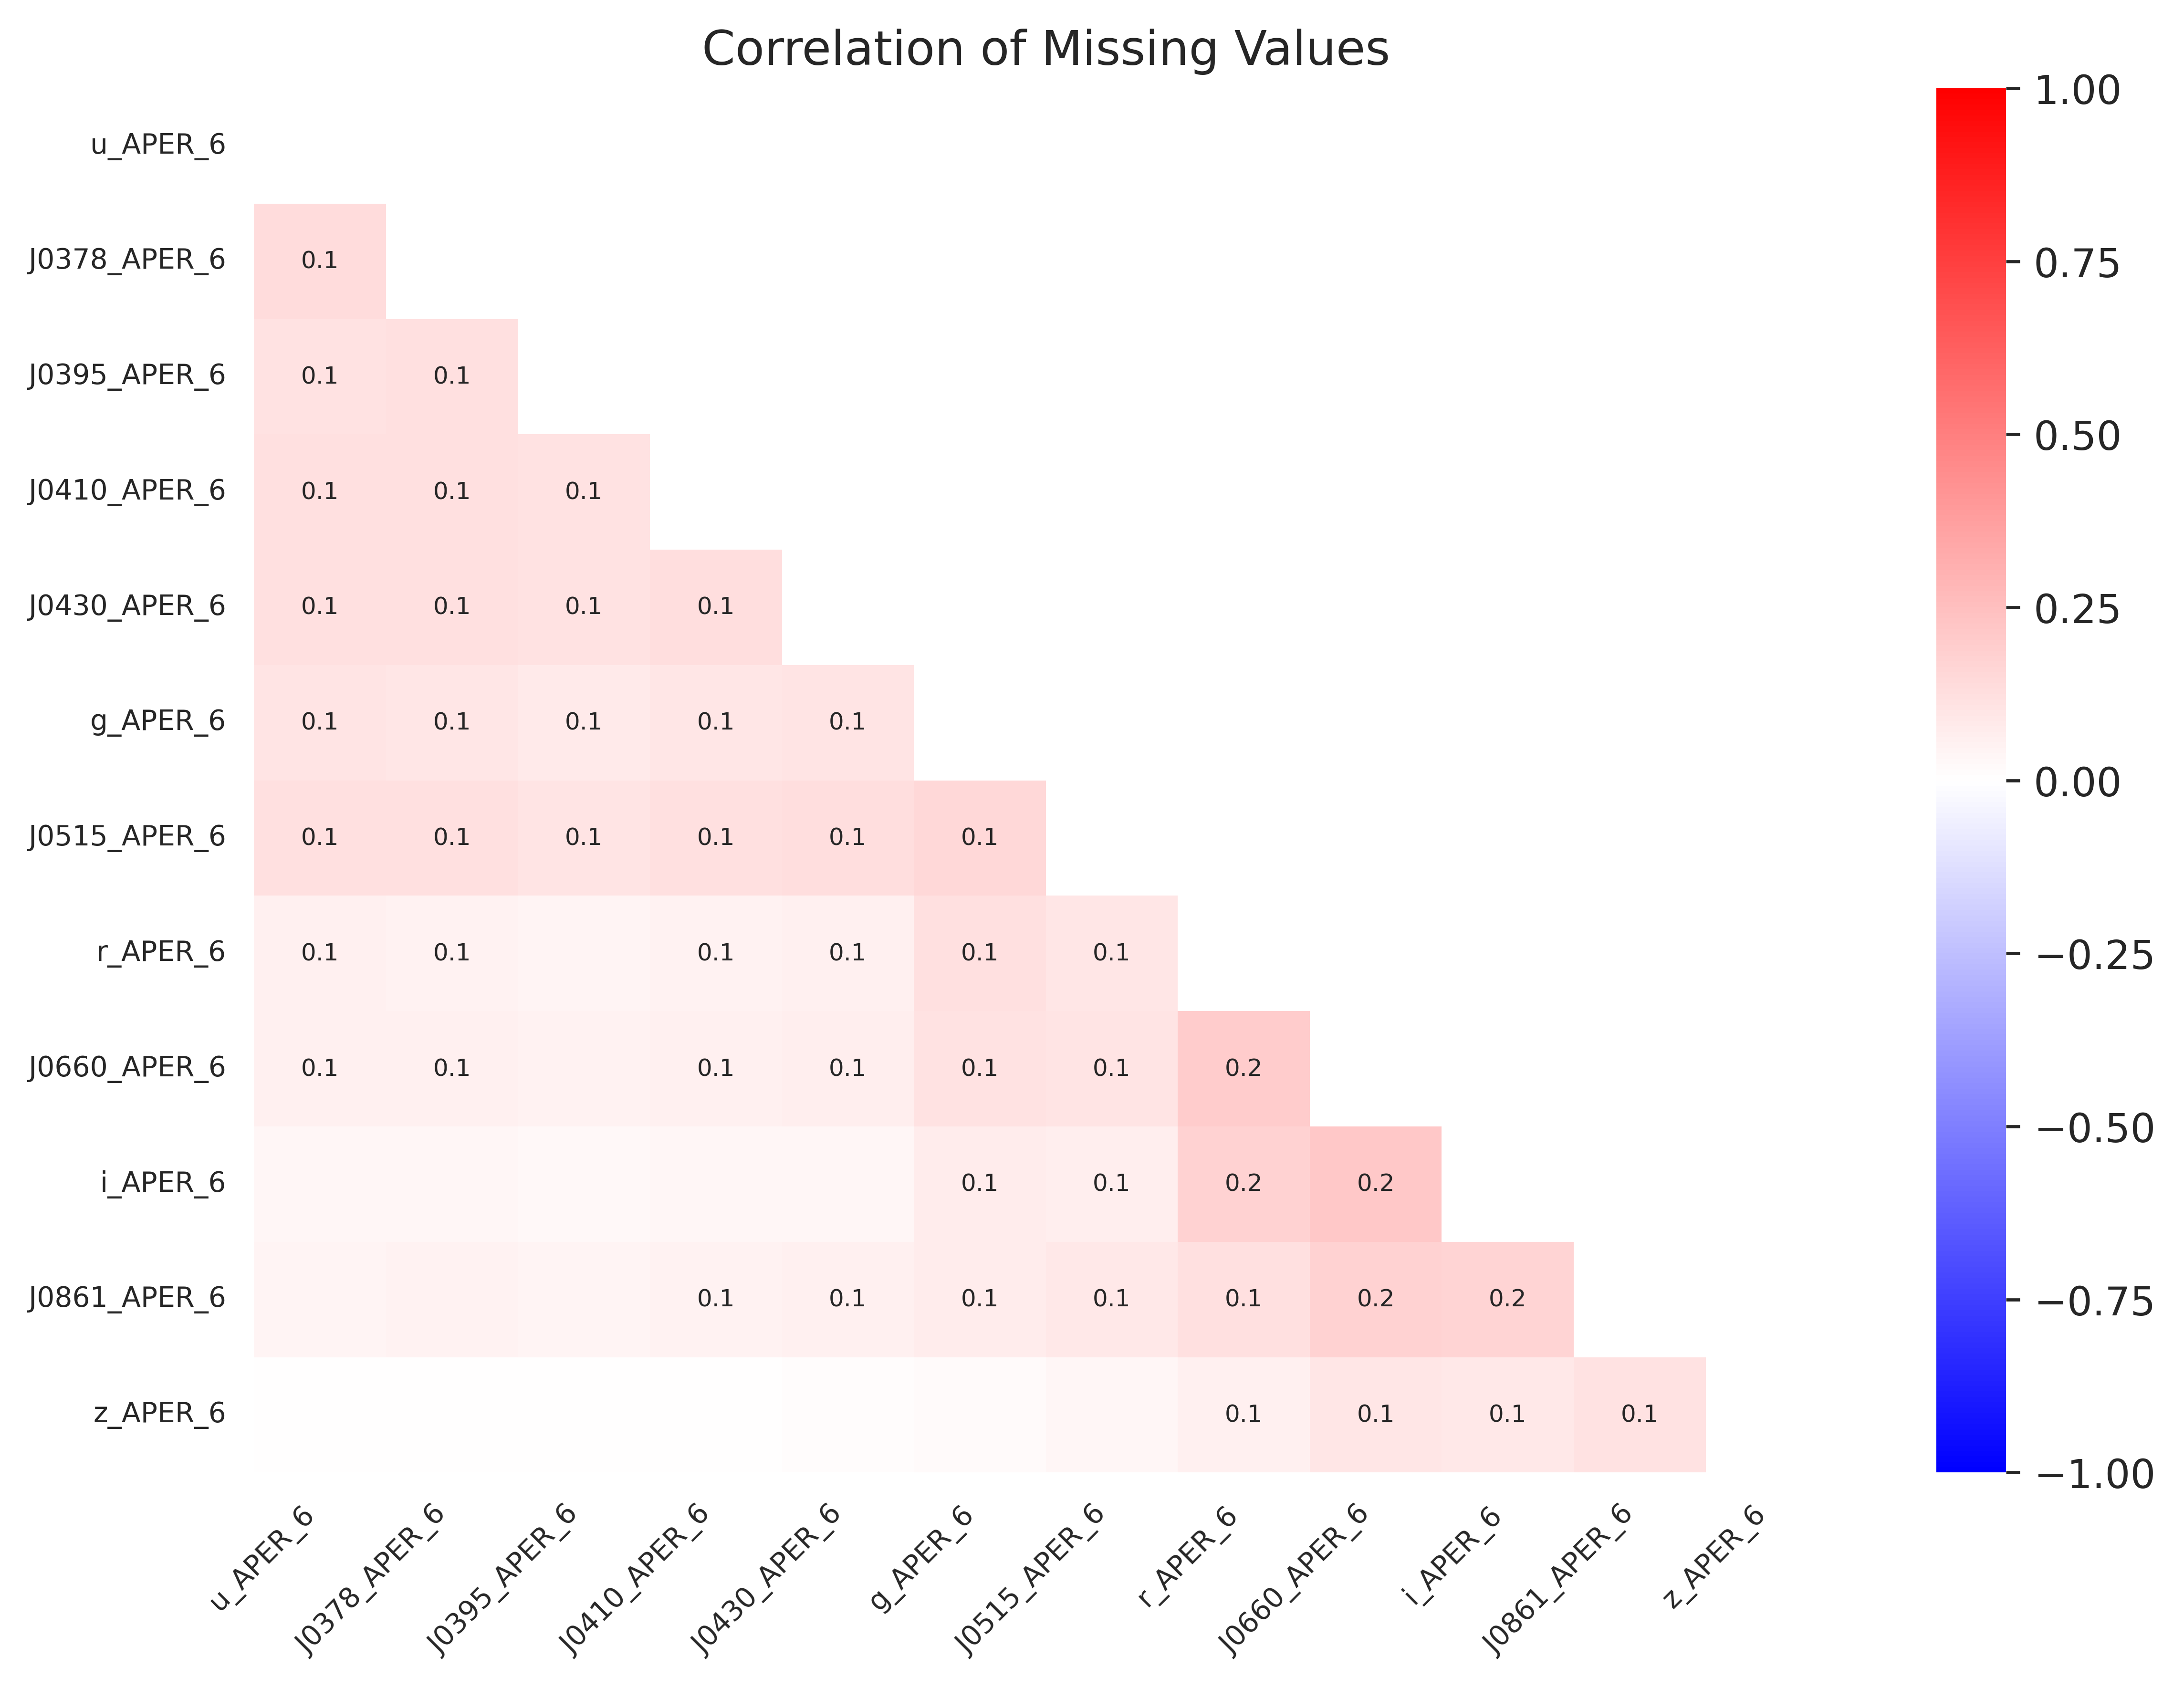
\includegraphics[width=0.85\columnwidth,angle=0]{matriz_correlacao.png}
    \caption[]{Matriz de correlação entre os valores faltantes. Cada célula contém o coeficiente de correlação entre os valores faltantes de duas bandas fotométricas. Cores em vermelho indicam correlação positiva, enquanto cores em azul indicam correlação negativa. Valores próximos de 0 indicam que os dados faltantes são independentes.}
    \label{matriz_correlacao}
    \end{center}
\end{figure}

Pela Figura \ref{matriz_correlacao}, observamos que a maioria dos valores faltantes não apresenta correlação significativa, sugerindo que os dados faltantes são independentes.

Existem várias técnicas para lidar com esses valores ausentes. Uma maneira simples e comum é remover os objetos que possuem algum dado faltante, mas isso pode gerar uma perda de informação para o treinamento. Outra alternativa é substituir os valores faltantes pela média dos valores restantes, mas isso pode introduzir um viés na nossa seleção. Há ainda a opção de utilizar algum valor padrão, como \texttt{NaN} (Not a Number) ou -1, porém, essa estratégia pode acabar confundindo o classificador, principalmente se esses valores não tiverem um significado claro para o modelo.

A técnica que adotamos para lidar com os valores faltantes foi a imputação dos dados utilizando o Método de Imputação Múltipla por Equações Encadeadas (MICE) (\citealp{MICE}). O MICE é um método de imputação que utiliza várias iterações de treinamento de modelos de aprendizado de máquina para prever os valores ausentes usando valores conhecidos de outras variáveis como preditores.

A fração de objetos da amostra, após os cortes descritos na seção \ref{subsec:cuts}, que possuem pelo menos 1, 2 ou 3 valores de magnitudes faltantes e que serão imputados, é de aproximadamente 27\%, 10\% e 3\%, respectivamente. Esses números evidenciam que uma parcela significativa dos objetos apresenta dados incompletos para as 12 magnitudes, ressaltando a importância do processo de imputação para garantir a qualidade e a consistência da análise.

\subsection{Treinando o modelo}\label{subsec:treinando_modelo}

Para o treinamento dos modelos, dividimos nossa amostra em duas classes: objetos compactos (classe 0) e objetos extensos (classe 1). Temos um total de 545.267 objetos.

Os classificadores são treinados com 80\% dos dados (436213 objetos) e testado com os 20\% restantes (109054 objetos), balanceado para garantir que a divisão dos dados entre treinamento e teste preserve a proporção das classes da variável. Isso significa que, se o conjunto de dados original tiver uma distribuição desbalanceada entre as classes (por exemplo, 70\% da classe 0 e 30\% da classe 1), essa mesma proporção será mantida tanto no conjunto de treino quanto no conjunto de teste. No conjunto de treinamento, temos 242.085 objetos classificados como pertencentes à classe 0 e 194.128 à classe 1. Já no conjunto de teste, temos 60.522 objetos da classe 0 e 48.532 da classe 1.

\raggedright
Utilizamos as 12 magnitudes da abertura APER\_6 corrigidas pela extinção (u\_APER\_6, J0378\_APER\_6, J0395\_APER\_6, J0410\_APER\_6, J0430\_APER\_6, g\_APER\_6, J0515\_APER\_6, r\_APER\_6, J0660\_APER\_6, i\_APER\_6, J0861\_APER\_6, z\_APER\_6) e as 66 combinações possíveis dessas magnitudes para formar as cores.

Os classificadores utilizados foram: K-Nearest Neighbors (KNN) e Random Forest (RF). Nos testes iniciais, tanto para o KNN quanto para o RF, a combinação das 12 magnitudes com as 66 cores apresentou resultados superiores em comparação ao uso isolado de apenas magnitudes ou apenas cores. No caso do KNN, a melhoria foi modesta, cerca de 0,5\% nos parâmetros de desempenho (Precisão e Completeza). Já para o RF, a melhoria foi mais significativa, com um aumento médio de aproximadamente 5\% nos mesmos parâmetros. Dessa forma, optamos por utilizar a combinação de ambas as informações para o treinamento do modelo.

Os dados foram normalizados usando a amostra de treino, ajustando sua distribuição para valores entre 0 e 1, de forma a garantir a correta aplicação das métricas de distância. Para isso, utilizamos a função de normalização MinMax do \textit{sklearn} em Python, que transforma os dados para o intervalo [0, 1] com base no conjunto de treinamento. Com esse modelo de normalização salvo, reaplicamos o mesmo modelo nos dados de teste, que também serão usados para as análises posteriores.

Nas próximas subseções, discutiremos os algoritmos escolhidos para treinar nossos modelos, o processo de seleção dos melhores hiperparâmetros e a avaliação do desempenho do classificador.

\subsubsection*{K-Nearest Neighbors (KNN)}\label{subsubsec:knn}
Inicialmente, testamos treinar o modleo de classificação, utilizamos o algoritmo K-Nearest Neighbors (KNN). O KNN é um algoritmo de aprendizado supervisionado que classifica um objeto com base em seus vizinhos mais próximos. Dada uma amostra de um conjunto de dados, ele irá calcular e avaliar as distâncias entre os objetos e, dada a classificação dos vizinhos mais próximos, o objeto será classificado de acordo. Para o treinamento, usamos a biblioteca \textit{scikit-learn} em Python, que implementa o algoritmo KNN.

O desempenho do KNN nos dará uma noção inicial da performance do modelo. O KNN é um algoritmo simples, mas eficaz, que pode ser utilizado como ponto de partida para a construção de modelos mais complexos. Ele é mais rápido de treinar e nos fornece uma ideia dos parâmetros que podem ser ajustados para o treinamento de modelos mais avançados.

A seleção dos melhores hiperparâmetros do modelo foi realizada por meio de uma busca com o método de \textit{GridSearchCV} da biblioteca \textit{sklearn} em Python, com validação cruzada de 5 folds (cv=5). Esse processo garantiu a otimização dos parâmetros \textit{n\_neighbors}, \textit{metric}, \textit{weights}, \textit{algorithm} e \textit{leaf\_size}, maximizando o desempenho do modelo durante o treinamento.

O modelo final selecionado foi treinado com 27 vizinhos, utilizando a distância de Manhattan como métrica, pesos proporcionais à distância, \textit{algorithm}='auto' e \textit{leaf\_size}=10.

\subsubsection*{Random Forest (RF)}\label{subsubsec:rf}
Para o treinamento com um modelo mais robusto, utilizamos o algoritmo Random Forest (RF). O RF é um método de aprendizado de máquina baseado em um conjunto de árvores de decisão. Durante o treinamento, o RF constrói diversas árvores de decisão independentes, cada uma treinada com uma amostra aleatória do conjunto de dados e de seus atributos. A previsão final é obtida pela média (para regressão) ou pela votação majoritária (para classificação) das previsões individuais das árvores.

O RF é amplamente utilizado em tarefas de classificação e regressão devido à sua capacidade de lidar com dados complexos, não lineares e de alta dimensionalidade. Além disso, ele é robusto a outliers e menos suscetível ao overfitting em comparação com modelos individuais, como árvores de decisão isoladas.

Para a seleção dos hiperparâmetros do modelo RF, definimos uma grade de parâmetros para otimização, incluindo: o número de árvores na floresta (\textit{n\_estimators}), a profundidade máxima das árvores (\textit{max\_depth}), o número mínimo de amostras necessárias para dividir um nó (\textit{min\_samples\_split}), o número mínimo de amostras necessárias para formar uma folha (\textit{min\_samples\_leaf}), o uso de \textit{bootstrap} e o número de características a serem consideradas ao procurar a melhor divisão (\textit{max\_features}).

Para encontrar a melhor combinação de hiperparâmetros, dado que para o RF temos um tempo de treino consideravelmetne maior, utilizamos a biblitoeca \textit{Optuna}, do Python, para otimização de hiperparâmetros. Essa biblioteca utiliza um algoritmo de otimização bayesiana para encontrar a melhor combinação de hiperparâmetros, permitindo uma busca mais eficiente em comparação com o método de \textit{GridSearchCV}.

A melhor combinação de hiperparâmetros encontrada foi: \textit{n\_estimators}=400, \textit{max\_depth}=15, \textit{min\_samples\_split}=6, \textit{min\_samples\_leaf}=3, \textit{bootstrap}=False e \textit{max\_features}=15.



\subsection{Análise do classificador}\label{subsec:analise_modelo}
Aplicando os modelos treinados nos dados de teste, podemos realizar e avaliar as previsões feitas pelos classificador. Para comparar o desempenho dos dois modelos, utilizamos as métricas de acurácia, precisão, completeza e F1-score.

A acurácia é definida como a fração das previsões corretas em relação ao total. 

\begin{equation}
    \text{Acurácia} = \frac{TP + TN}{TP + TN + FP + FN}
\end{equation}

A precisão (ou pureza) é a fração de verdadeiros positivos em relação ao total de positivos. 

\begin{equation}
    \text{Precisão} = \frac{TP}{TP + FP}
    \label{eq:precisao}
\end{equation}

A completeza é a fração de verdadeiros positivos em relação ao total de positivos previstos.

\begin{equation}
    \text{Completeza} = \frac{TP}{TP + FN}
    \label{eq:completeza}
\end{equation}

O F1-score é a média harmônica entre precisão e completeza.

\begin{equation}
    \text{F1-score} = 2 \times \frac{\text{Precisão} \times \text{Completeza}}{\text{Precisão} + \text{Completeza}}
\end{equation}

Para ilustrar o desempenho do classificador, usamos ainda a curva AUC-ROC, amplamente utilizada para modelos de classificação binária. A ROC (Receiver Operating Characteristic) exibe a relação entre a sensibilidade (taxa de verdadeiros positivos) e a taxa de falsos positivos. A AUC (Área Sob a Curva) resume a performance em um único valor. Uma AUC de 0.5 indica classificação aleatória, enquanto 1.0 representa um modelo perfeito.

Essas são as métricas mais populares adotadas em tarefas de classificação binária. Porém, essas medidas estatísticas podem mostrar resultados excessivamente otimistas, especialmente em conjuntos de dados desbalanceados. Uma métrica adicional que usaremos é o coeficiente de correlação de Matthews (MCC), definido por:

\begin{equation}
    \text{MCC} = \frac{TP \times TN - FP \times FN}{\sqrt{(TP + FP)(TP + FN)(TN + FP)(TN + FN)}}
\end{equation}

Ela é uma métrica estatística que produz uma pontuação alta apenas se a previsão obtiver bons resultados em todas as quatro categorias da matriz de confusão, proporcionalmente tanto ao tamanho dos elementos positivos quanto ao tamanho dos elementos negativos no conjunto de dados. Os valores do MCC variam de -1 a 1, em que 1 indica uma previsão perfeita, 0 indica uma previsão aleatória e -1 indica uma previsão totalmente incorreta.

A Tabela \ref{metricas_modelo_knn} mostra as métricas obtidas para o modelo KNN treinado. Já a Tabela \ref{metricas_modelo_rf} mostra as métricas obtidas para o modelo RF treinado.

\begin{table}[!ht]
    \centering
    \caption{Classificação binária - Métricas modelo KNN}
    \begin{tabular}{lccc}
        \toprule
        Classe & Precisão & Completeza & F1-Score \\
        \midrule
        0 & 0.92 & 0.88 & 0.90 \\
        1 & 0.86 & 0.91 & 0.88 \\
        \midrule
        \multicolumn{3}{l}{AUC-ROC} & 0.95 \\
        \multicolumn{3}{l}{Coeficiente de Correlação de Matthews (MCC)} & 0.78 \\
        \bottomrule
    \end{tabular}
    \label{metricas_modelo_knn}
\end{table}


\begin{table}[!ht]
    \centering
    \caption{Classificação binária - Métricas modelo RF}
    \begin{tabular}{lccc}
        \toprule
        Classe & Precisão & Completeza & F1-Score \\
        \midrule
        0 & 0.95 & 0.90 & 0.92 \\
        1 & 0.89 & 0.94 & 0.91 \\
        \midrule
        \multicolumn{3}{l}{AUC-ROC} & 0.97 \\
        \multicolumn{3}{l}{Coeficiente de Correlação de Matthews (MCC)} & 0.84 \\
        \bottomrule
    \end{tabular}
    \label{metricas_modelo_rf}
\end{table}

Na Figura \ref{confusion_matrix}, temos a matriz de confusão dos modelos, mostrando a quantidade de verdadeiros positivos (TP), verdadeiros negativos (TN), falsos positivos (FP) e falsos negativos (FN) obtidos.

\begin{figure}[!ht]
    \centering
    \captionsetup{justification=centering}
    \begin{subfigure}[b]{0.48\textwidth}
        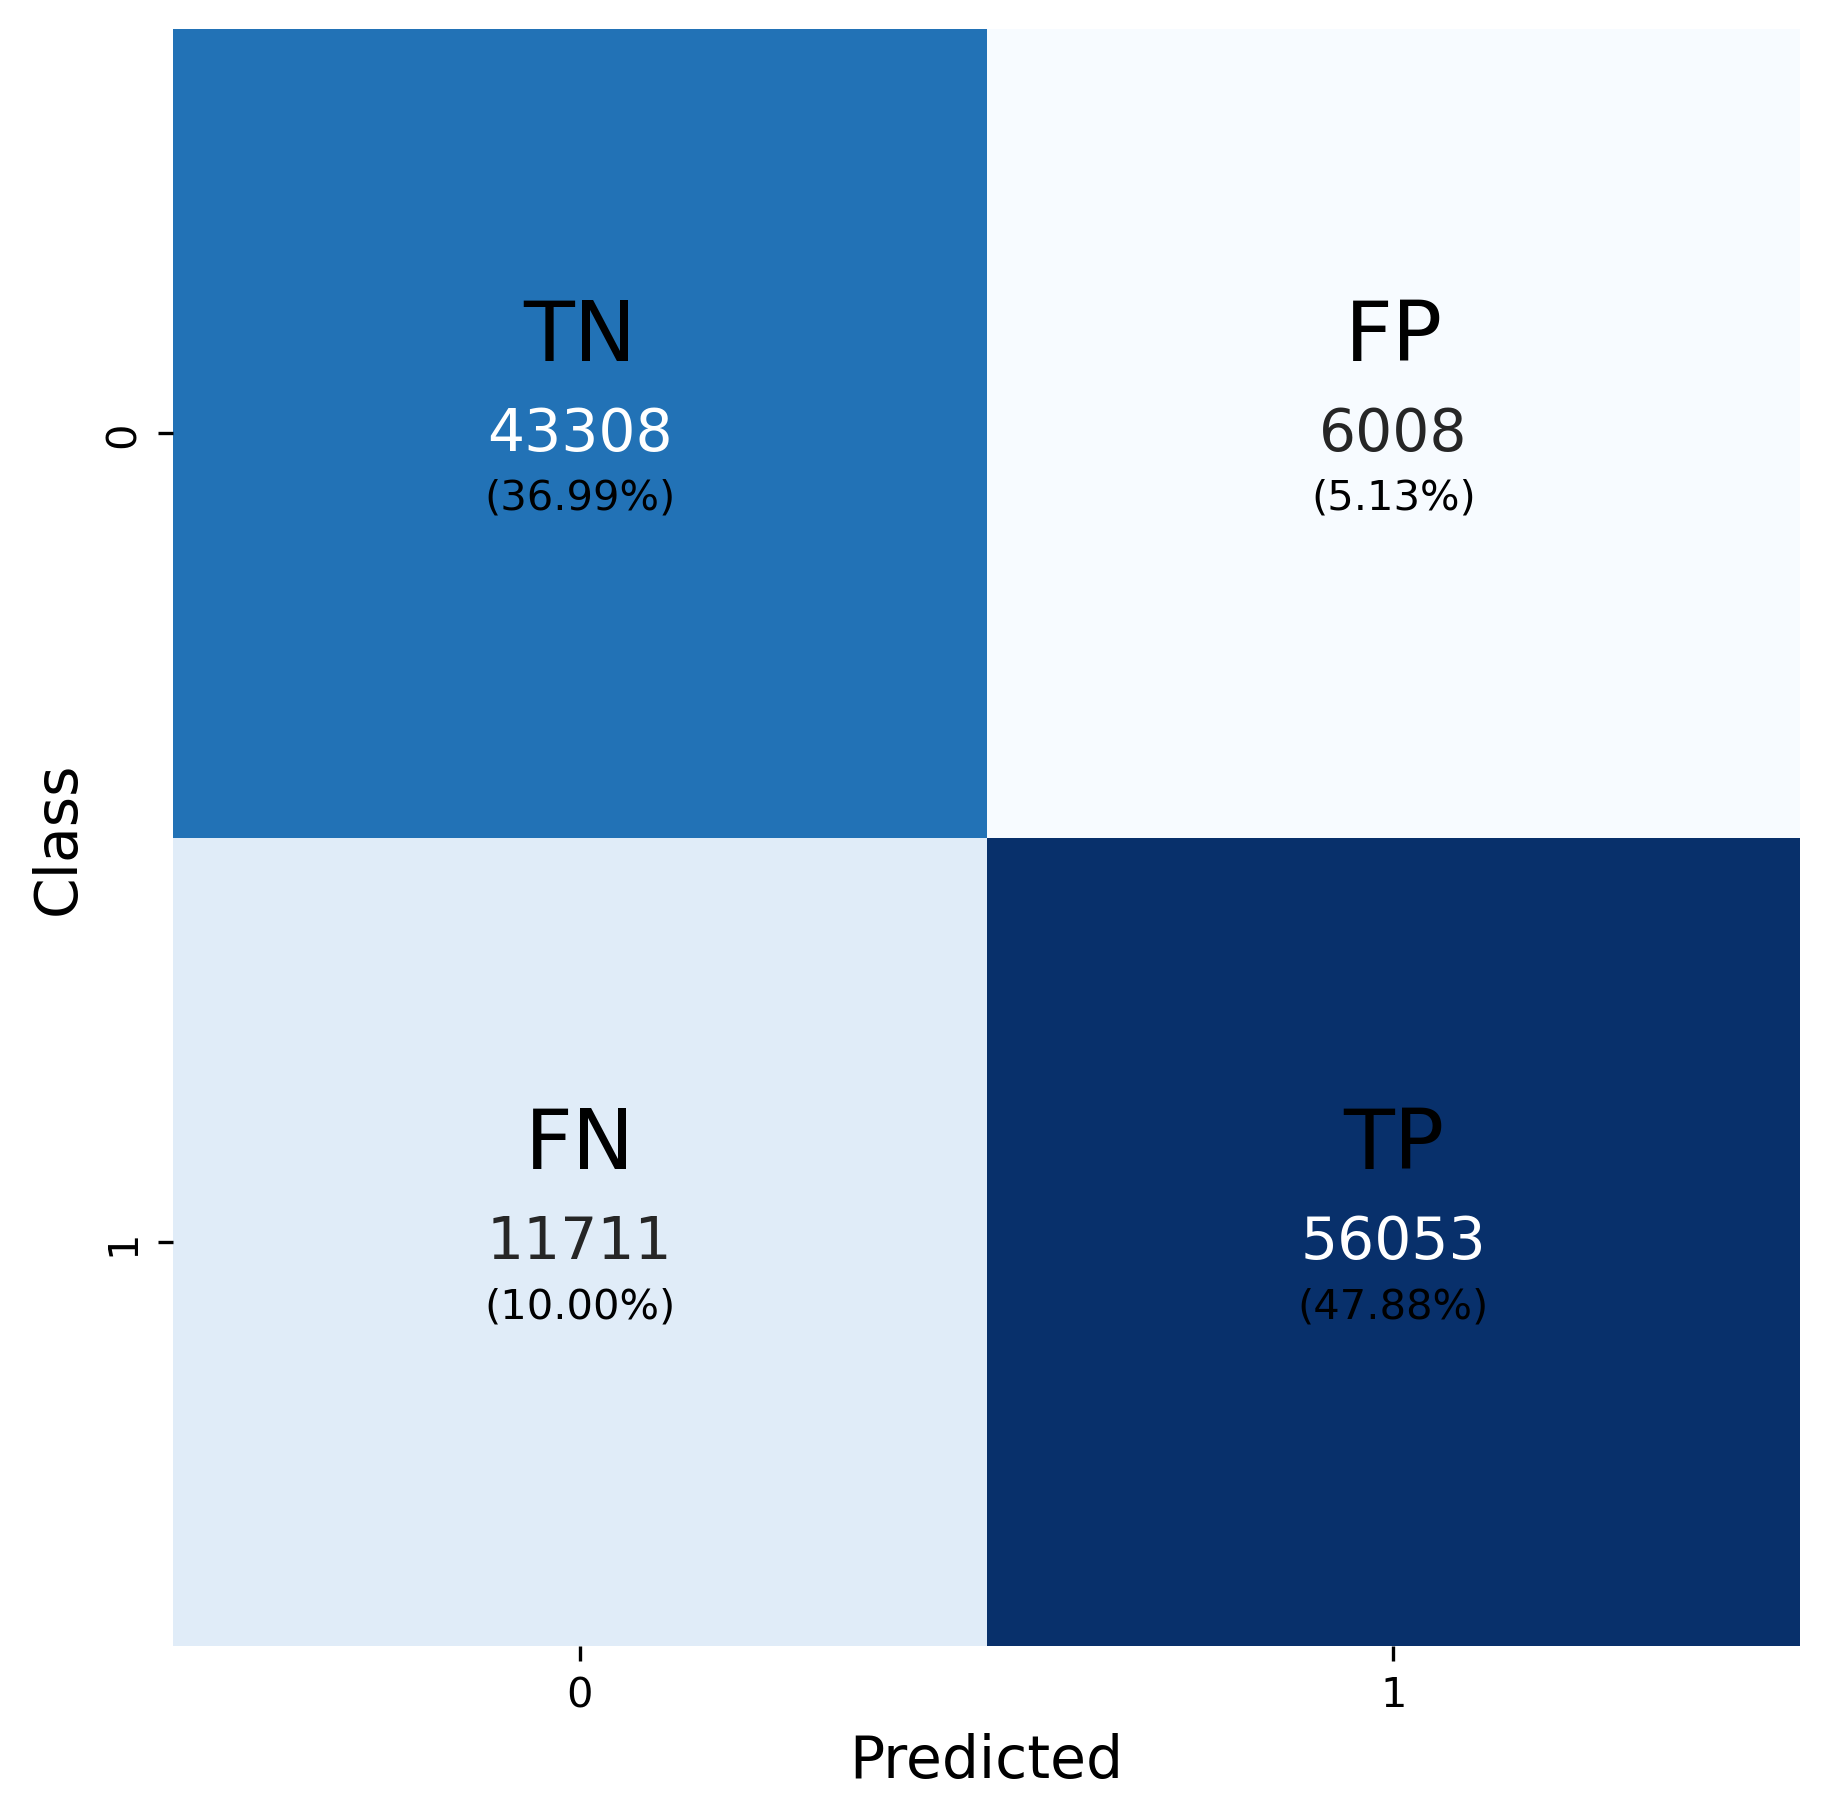
\includegraphics[width=\textwidth]{confusion_matrix_knn.png}
        \caption{Modelo KNN}
    \end{subfigure}
    \begin{subfigure}[b]{0.48\textwidth}
        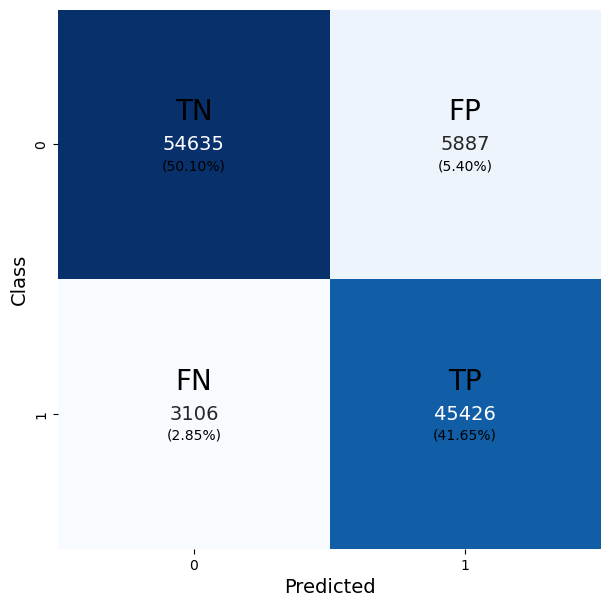
\includegraphics[width=\textwidth]{confusion_matrix_rf.png}
        \caption{Modelo RF}
    \end{subfigure}
    \caption{Matriz de confusão do modelo KNN (a) e o modelo RF (b). A diagonal principal representa os valores corretamente classificados, enquanto os valores fora da diagonal principal representam os erros de classificação das classes 0 e 1.}
    \label{confusion_matrix}
\end{figure}

Pelos resultados das métricas adotadas, e também pela matrizes de confusão, podemos observar que o modelo RF apresenta um desempenho superior ao modelo KNN. Assim, optamos por utilizar o modelo RF para a classificação dos objetos compactos e extensos.

Muitos dos objetos tiveram classificação correta, como podemos ver na diagonal principal das matrizes de confusão da Figura \ref{confusion_matrix}. Porém, cabe ressaltar que nem todos os objetos do conjunto de teste eram estrelas ou galáxias, mas sim, majoritariamente, mais de cada um deles nas classes de compactos e extensos, respectivamente. Assim, é esperado que algumas classificações sejam feitas de forma errada, e é nessa proposta que o modelo foi treinado: encontrar aqueles com maior probabilidade de serem extensos, mas que fazem parte do conjunto dos compactos.

Os resultados obtidos pelo RF têm valores de precisão, completeza e F1-score acima de 0,89 para ambas as classes. A AUC-ROC de 0,97 indica que o modelo é capaz de distinguir entre as duas classes com boa precisão, dadas as limitações dos conjuntos de treinamento. O coeficiente de correlação de Matthews (MCC) de 0,84 é um indicativo de que o modelo é capaz de prever corretamente a maioria dos objetos.

Foram realizadas as previsões de probabilidade de ser da classe 1 (objetos extensos) para toda a amostra que estaremos analisando na busca (amostra de treino e amostra de teste). A Figura \ref{probabilidade_extensos_fwhm} mostra a distribuição de \textit{FWHM} na banda \textit{r} dos objetos com classificação como estrela ou galáxia do GAIA DR3 com probabilidade maior que 90\%. Sobreposta na imagem, temos matrizes de confusão do classificador para diferentes intervalos de \textit{FWHM}.

\begin{figure}[!ht]
    \centering
    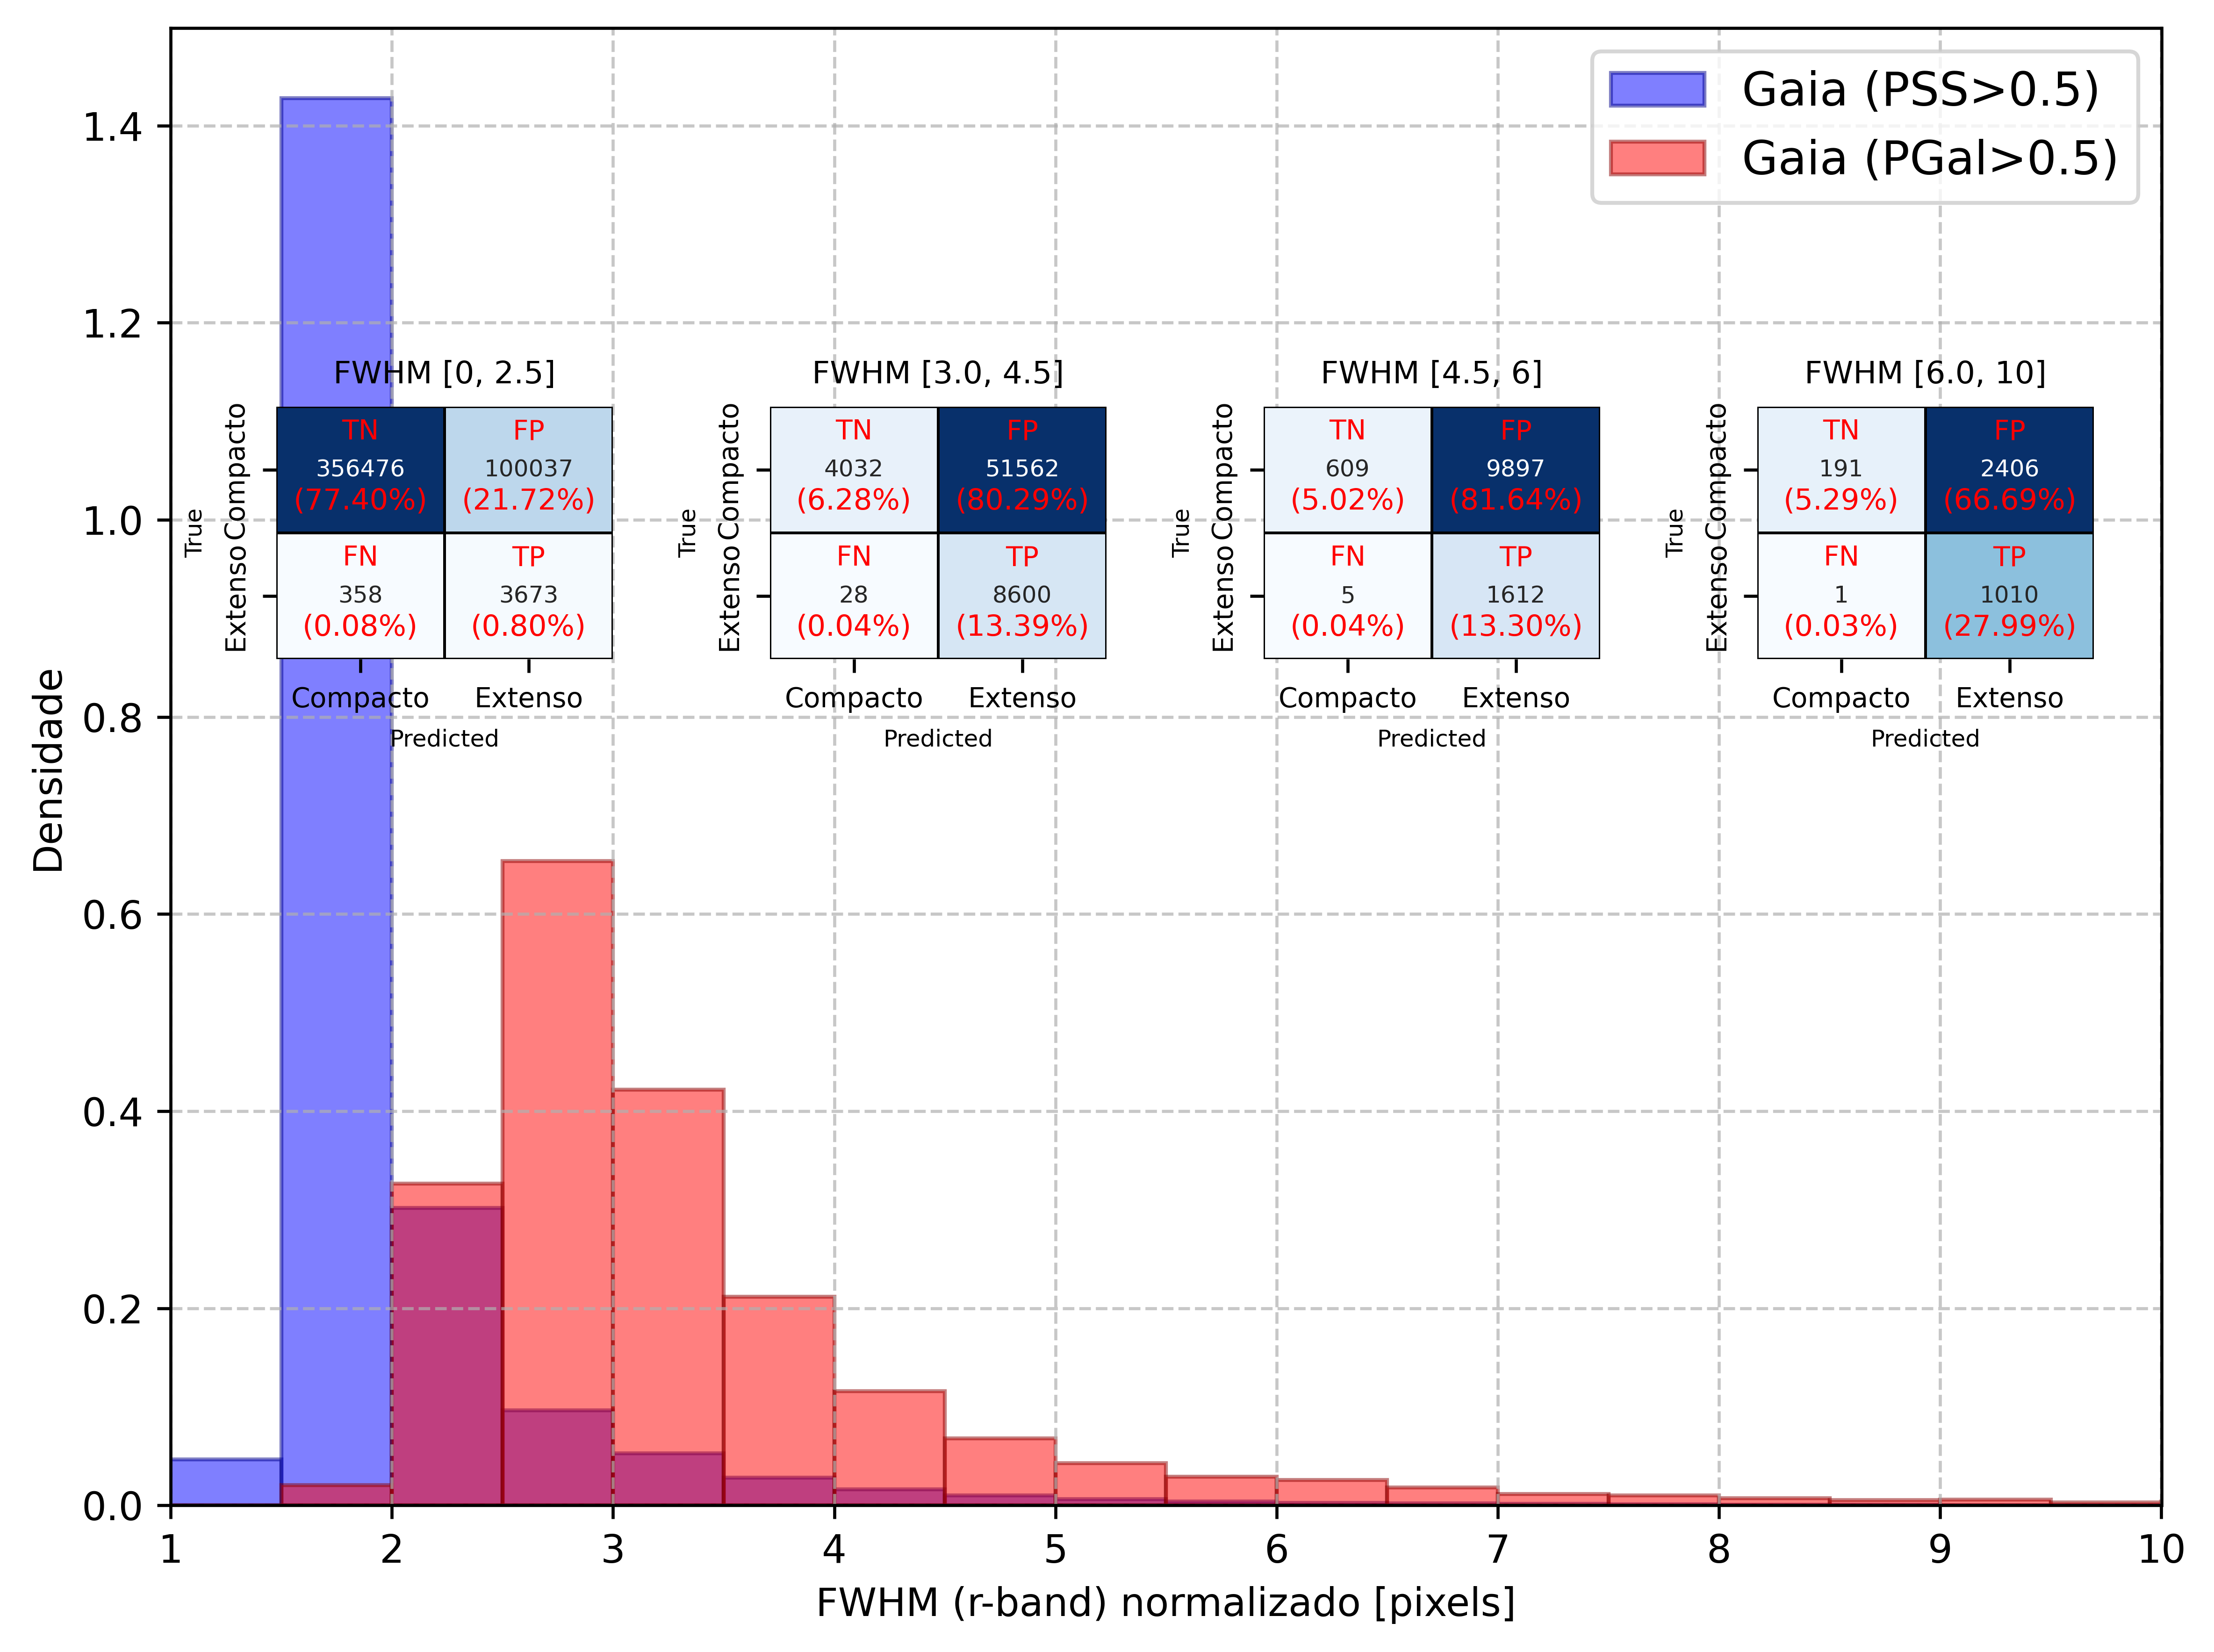
\includegraphics[width=1.\columnwidth,angle=0]{distribution_of_stars_and_galaxies_with_cm.png}
    \caption[]{Distribuição de \textit{FWHM (r-band)} para objetos da amostra com classificação estrela-galáxia do GAIA DR3 com probabilidade maior que 90\%. As matrizes de confusão do classificador KNN para diferentes intervalos de \textit{FWHM} estão sobrepostas. O classificador dá a probabilidade de ser da classe 1 (extensos) para cada objeto. }
    \label{probabilidade_extensos_fwhm}
\end{figure}

O comportamento do classificador nas matrizes de confusão mostra que, para as regiões de \textit{FWHM} menores (entre [0, 2.5]), onde há uma maior concentração de estrelas, observa-se uma alta taxa de classificação para objetos do tipo compacto. Já para objetos com \textit{FWHM} maiores, o classificador mostra uma tendência de classificá-los como extensos, o que é esperado, já que esses objetos são menos prováveis de serem estrelas. Para objetos com \textit{FWHM} nas faixas de sobreposição, o desempenho do classificador é misto, refletindo a dificuldade em separar essas classes na região. Porém, é possível observar uma transição gradual entre as classes, consistente com os picos das distribuições de \textit{FWHM}.

Ilustrando ainda o resultado da classificação, apresentamos na Figura \ref{predic_colored} o mesmo gráfico da Figura \ref{amostra_treino} para os objetos da amostra de teste, coloridos de acordo com a probabilidade de serem objetos extensos pelo modelo RF. A cor azul indica uma probabilidade baixa, enquanto a cor vermelha indica uma probabilidade alta. 

Do classificador para a amostra, tivemos um total de 1.803.561 objetos analisados, dos quais 1.411.903 (78,28\%) apresentaram probabilidade acima de 50\% de serem extensos, enquanto 391.658 (21,72\%) apresentaram probabilidade abaixo de 50\%. Entre os objetos com probabilidade acima de 50\% de serem extensos, 311.846 (17,29\%) possuem \textit{FWHM} menor que 2,5 pixels, ou seja, são objetos compactos que têm mais de 50\% de chance de serem semelhantes à amostra de objetos extensos.

\begin{figure}[!ht]
    \centering
    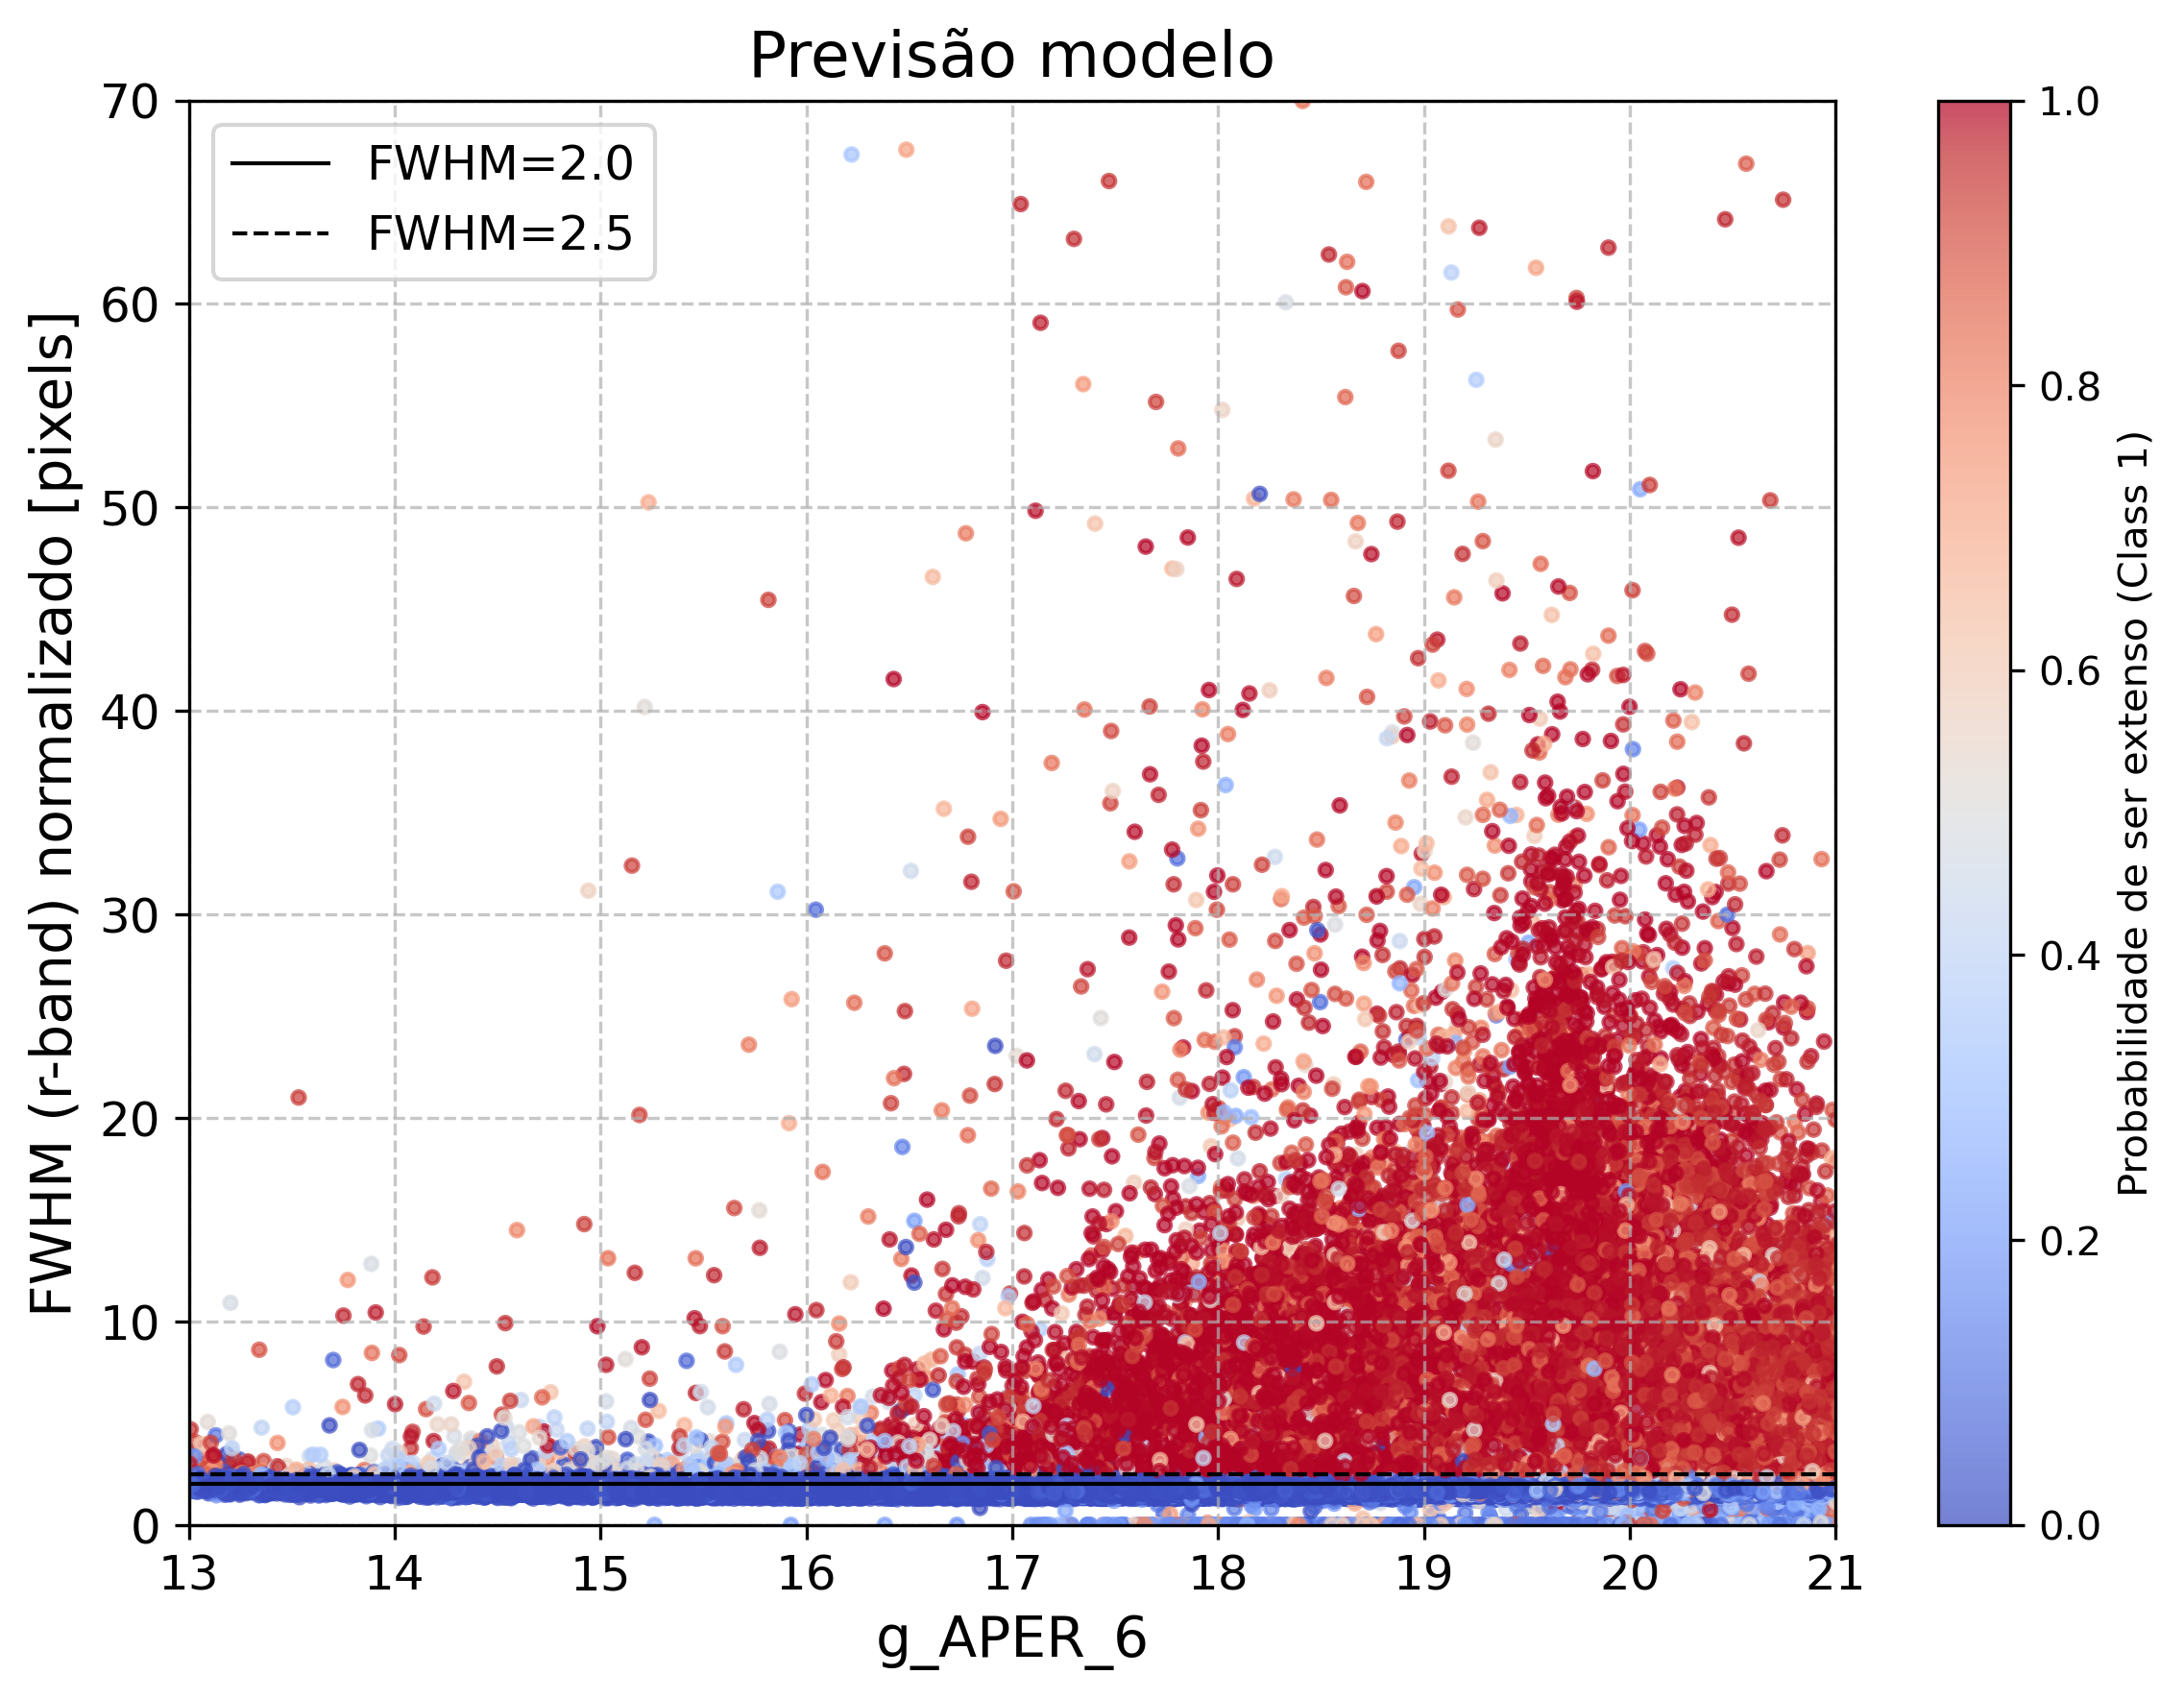
\includegraphics[width=1.\columnwidth,angle=0]{predic_colored.png}
    \caption[]{Distribuição da Largura Total na Metade Máxima (\textit{FWHM} r-band) em função da magnitude \textit{g\_APER\_6} para objetos da amostra de teste, coloridos de acordo com a probabilidade de serem objetos extensos (Classe 1) pelo modelo. Divisão das classes: compactos (\textit{FWHM}$\leq$2 pixels) e extensos (\textit{FWHM}$\geq$2.5 pixels).}
    \label{predic_colored}
\end{figure}

A probabilidade dos objetos serem da classe 1 (objetos extensos) para as UCDs conhecidas na amostra é apresentada na Tabela \ref{ucds_predict}.

\begin{table}[H]
    \centering
    \caption{Classificação do modelo para a classe 1 (objetos extensos) das UCDs na amostra de análise}  
    \begin{tabular}{lc}
        \toprule
        Nome & Predição modelo RF \\
        \midrule
        UCD3 & 0.36 \\
        UCD1 & 0.98 \\
        F-24 & 0.99 \\
        UCD5 & 0.38 \\
        F-1a & 0.11 \\
        F-9 & 0.87 \\
        F-5 & 0.53 \\
        F-6 & 0.89 \\
        F-7 & 0.70 \\
        F-12 & 0.73 \\
        F-11 & 0.97 \\
        F-34 & 0.98 \\
        F-22 & 0.93 \\
        % F-53 & 0.96 \\
        % F-51 & 0.96 \\
        % F-59 & 0.92 \\
        \bottomrule
    \end{tabular}
    \label{ucds_predict}
\end{table}

Das 13 UCDs presentes, 9 foram classificadas com uma predição acima de 70\%, e 2 com classificação muito pouco provável. 

% \subsection*{Previsões para aglomerados globulares}\label{subsec:predicoes_gc}


% Como mencionado neste trabalho, parte das UCDs estudadas possivelmente têm sua formação associada a aglomerados globulares (Globular Clusters, GCs). A classificação adotada para distinguir UCDs de GCs, conforme descrito na seção \ref{subsec:cuts}, considera objetos com \textit{g}$\leq$21 como UCDs e aqueles com \textit{g}$>$21 como GCs.

% Para o classificador RF, podemos obejtsar o seu comportamento e classiicação para GCs na nossa amostra. Para Uma lsita de GCs em Fornax, usmaos os dados vindo de \cite{Saifollahi_2021}, que apresenta uma lista de GCs/UCDs conhecidas na região de Fornax. Removemos 

\section{Redshifts fotométricos}\label{sec:zphot}

A determinação de redshifts é uma etapa importante para identificar a localização dos objetos no universo. Nesse trabalho, os redshifts fotométricos (\textit{$z_{phot}$}) permitem que estimemos a distância dos objetos de forma eficiente e em larga escala, utilizando apenas dados fotométricos. Essa abordagem é especialmente útil quando não há disponibilidade de redshifts espectroscópicos (\textit{$z_{spec}$}). A utilização de redshifts fotométricos têm o objetivo de filtrar objetos que não pertencem ao aglomerado de Fornax, reduzindo a contaminação por objetos de fundo.

% Com os objetos filtrados de candidatas, calculamos os redshifts fotométricos (\textit{$z_{phot}$}) dos objetos, selecionando aqueles nos intervalos mais compatíveis com Fornax.

É possível encontrar redshifts fotométricos para parte dos objetos da nossa amostra em outros trabalhos da literatura, assim como em catálogos da própria colaboração S-PLUS \citep{erik_photoz_2024}. Porém, para a busca neste projeto, utilizamos dados com a redução da fotometria do S-PLUS diferentes dos utilizados para os \textit{$z_{phot}$} disponíveis. Assim, mesmo que vindos do mesmo catálogo, uma pequena parte dos objetos na nossa amostra não tem redshifts fotométricos disponíveis. Dos 2900926 objetos iniciais da nossa amostra, 290637 objetos não têm redshifts fotométricos disponíveis em \citep{erik_photoz_2024}.

Abordagens comuns para a estimativa de \textit{$z_{phot}$} incluem o ajuste baseado em modelos espectrais (\textit{template fitting}) e técnicas de aprendizado de máquina. O método de \textit{template fitting} apresenta a vantagem de permitir extrapolações, sendo útil para objetos cujas propriedades não estão bem representadas em amostras conhecidas. Já o aprendizado de máquina tende a ser mais eficiente e preciso quando treinado com um conjunto de dados representativo, embora sua capacidade de generalização seja limitada fora do intervalo coberto pelo treinamento. Além disso, algoritmos de aprendizado de máquina costumam oferecer tempos de inferência mais rápidos, o que os torna especialmente atrativos em contextos com grandes volumes de dados.

Aqui optamos por utilizar o método de aprendizado de máquina para calcular \textit{$z_{phot}$}. Para isso, empregamos modelos de regressão utilizando o algoritmo Random Forest (RF), implementado em Python. No caso da regressão, o RF cria uma floresta de árvores de decisão, onde cada uma delas é treinada com uma amostra aleatória do conjunto inicial dos dados e de seus atributos. A previsão para o valor de \textit{$z_{phot}$} é feita pela média das previsões de cada árvore.

Para a seleção da amostra de treino, utilizamos o mesmo catálogo de Fornax usado anteriormente, com os dados de fotometria do S-PLUS provenientes de \cite{haack2024splusfornaxprojectsfp} (\textit{Run 1}). Ou seja, temos os mesmos dados descritos na seção \ref{sec:Fornax_data}, com as 12 magnitudes corrigidas pela extinção (como descrito na seção \ref{sec:Coeficientes_ext}).

Dessa amostra, selecionamos os objetos com redshifts espectroscópicos disponíveis, provenientes do catálogo \cite{Lima_2024}. Cortamos os objetos em um intervalo de redshifts de 0.002 a 0.5, dessa maneira evitamos boa parte das estrelas (com redshifts menores) e galáxias muito distantes de Fornax. Cortamos também em um intervalo de magnitude de \textit{r\_APER\_6}>15 e \textit{r\_APER\_6}$\leq$21, evitando objetos muito brilhantes e saturados, e objetos com baixa qualidade de medição, respectivamente.

Removemos também os objetos com medições faltantes em alguma das 12 magnitudes das aberturas \textit{APER\_6}, resultando em uma amostra final com 12.296 objetos.

Para o treinamento, os melhores resultados a princípio se deram com a utilização das combinações das 66 cores das 12 magnitudes de abertura \textit{APER\_6}. Assim, treinamos o modelo fornecendo o redshift espectroscópico (\textit{$z_{spec}$}) como variável alvo e as 66 cores como variáveis preditoras.

% A seleção dos melhores hiperparâmetros foi realizada com validação cruzada de 5 folds, otimizando os parâmetros \textit{n\_neighbors}, \textit{metric}, \textit{weights}, \textit{algorithm} e \textit{leaf\_size}.

Dividimos a amostra em 80\% para treino e 20\% para teste. O conjunto de dados foi normalizado usando a amostra de treino, ajustando sua distribuição para valores entre 0 e 1 pela função MinMax do Python. 

A Figura \ref{zphot_zspec} mostra a comparação entre os redshifts espectroscópicos (\textit{$z_{spec}$}) e fotométricos (\textit{$z_{phot}$}) para a amostra de treino. A linha tracejada representa a relação 1:1 entre os redshifts, enquanto a linha contínua representa a relação ajustada pelo modelo de regressão.

\begin{figure}[!ht]
    \centering
    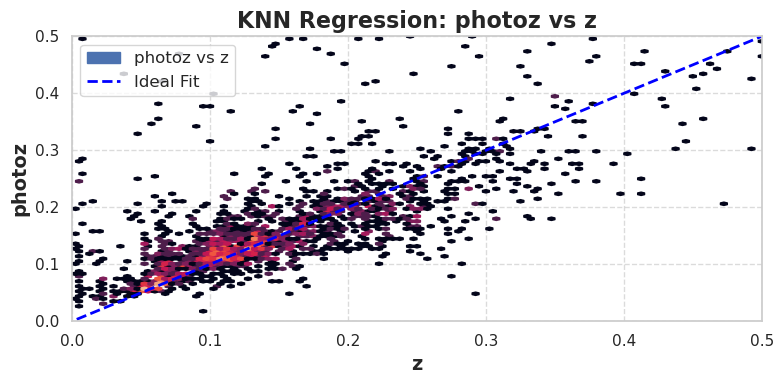
\includegraphics[width=1.\columnwidth,angle=0]{zphot_zspec.png}
    \caption[]{Resultados da regressão com o algoritmo Random Forest (RF) para estimar os redshifts fotométricos (\textit{$z_{phot}$}) em relação aos redshifts espectroscópicos (\textit{$z_{spec}$}). Na parte superior, o gráfico de dispersão compara \textit{$z_{phot}$} vs \textit{$z_{spec}$}. A linha azul tracejada representa o ajuste ideal (\textit{$z_{phot}$} = \textit{$z_{spec}$}). A densidade de pontos é representada por um gradiente de cores, com áreas mais densas indicadas em tons mais claros.}
    \label{zphot_zspec}
\end{figure}

Percebemos pela Figura \ref{zphot_zspec} que o modelo de regressão foi capaz de estimar os redshifts fotométricos com certa precisão. As métricas que adotamos para avaliar o desempenho do modelo foram o erro quadrático médio (EQM), o $R^2$ o $\sigma_{nmad}$ e a fração de outliers (Fout). O EQM é uma medida da média dos erros quadráticos entre os valores previstos e os valores reais. O $R^2$ é uma medida de quão bem os dados se ajustam ao modelo, variando de 0 a 1, onde 1 indica um ajuste perfeito. O $\sigma_{nmad}$ é uma medida robusta de dispersão que quantifica a variação dos resíduos em relação à mediana. A fração de outliers (Fout) é a proporção de previsões que estão além de um certo limite em relação aos valores reais.

Os resultados obtidos para essas métricas foram: EQM = 0,05, $R^2$ = 0,6, $\sigma_{nmad}$ = 0,03 e Fout = 0,08. Embora os valores indiquem uma precisão moderada, o modelo apresenta algumas estimativas com erros maiores, especialmente para redshifts mais elevados. É importante destacar que o objetivo principal deste modelo não é fornecer redshifts altamente precisos para todos os objetos, mas sim identificar aqueles com redshifts compatíveis com o aglomerado de Fornax. Dessa forma, mesmo com a presença de erros, o modelo é útil para filtrar objetos com maior probabilidade de pertencerem ao fundo, proporcionando um ganho significativo na seleção de candidatos.

Aplicando o modelo para as UCDs conhecidas em Fornax, obtivemos os resultados apresentados na Tabela \ref{ucds_zphot}, juntamente com os redshifts fotométricos fornecidos por \cite{erik_photoz_2024} (\textit{zml}). Para os objetos que possuem redshifts fotométricos disponíveis em \citep{erik_photoz_2024}, observamos que esses valores são mais precisos e compatíveis com os esperados para Fornax, em comparação com os redshifts fotométricos estimados pelo nosso modelo.

Essa diferença de desempenho é compreensível, dado que o modelo de \cite{erik_photoz_2024} utiliza uma abordagem mais robusta, baseada em uma amostra maior de objetos com redshifts espectroscópicos conhecidos, o que proporciona maior confiabilidade nos resultados. Por outro lado, nosso modelo, embora tenha apresentado resultados razoáveis, é limitado pela menor quantidade de dados disponíveis para o treinamento.

Portanto, concluímos que, sempre que possível, os cortes baseados em redshifts fotométricos devem ser realizados utilizando os valores de \cite{erik_photoz_2024}. Para os casos em que esses dados não estão disponíveis, utilizaremos os redshifts fotométricos estimados pelo nosso modelo como uma alternativa, cientes de suas limitações.

\begin{table}[!ht]
    \centering
    \caption{Aplicação do modelo de regressão para estimativas de redshifts fotométricos para UCDs conhecidas na amostra de análise de Fornax (\textit{$z_{phot}$}), junto com as previsões de \citep{erik_photoz_2024} (\textit{zml}), para aqueles objetos que tinham dados presentes e o redshift espectroscópico (\textit{$z_{spec}$}) disponível.}
    \begin{tabular}{lccc}
        \toprule
        Nome & \textit{$z_{phot}$} & \textit{zml} & \textit{$z_{spec}$}\\
        \midrule
        UCD3 & 0.07 & 0.03 & 0.0053\\
        UCD1 & 0.09 & 0.08 & 0.0052\\
        F-24 & 0.08 & 0.04 & 0.0062\\
        UCD5 & 0.03 & 0.04 & 0.0045\\
        F-1a & 0.21 & -- & 0.0042\\
        F-9 & 0.09 & 0.07 & 0.0058\\
        F-5 & 0.06 & -- & 0.0057\\
        F-6 & 0.10 & -- & 0.0037\\
        F-7 & 0.19 & 0.16 & 0.0050\\
        F-12 & 0.07 & -- & 0.0055\\
        F-11 & 0.10 & -- & 0.0059\\
        F-34 & 0.07 & -- & 0.0054\\ 
        F-22 & 0.09 & 0.06 & 0.0034\\
        F-53 & 0.31 & -- & 0.0020\\
        F-51 & 0.10 & -- & 0.0041\\
        F-59 & 0.06 & -- & 0.0060\\
        \midrule
    \end{tabular}
    \label{ucds_zphot}
\end{table}

Nosso objetivo não é estimar redshifts precisos para todos os objetos, mas sim aplicar um corte que nos ajude a remover objetos com maiores chances de serem do fundo. Sabendo que o redshift de Fornax é de aproximadamente $0.005$\footnote{https://simbad.u-strasbg.fr/simbad/sim-id?Ident=Fornax+Cluster}, e observando os redshifts fotométricos estimados para as UCDs conhecidas, podemos adotar um corte conservador para os redshifts fotométricos, com uma margem otimista para o erro.

\section{Seleção das candidatas}\label{cap:selecao_candidatas}
Para a seleção das candidatas, queremos primeiramente criar uma subamostra dos dados de Fornax, contendo os objetos compactos de nosso interesse. A partir dessa amostra, iremos selecionar pelas probabilidades de serem extensos (classe 1). Para amostra inicial, depois dos cortes feitos da seção \ref{subsec:cuts}, temos um total de 1.803.561 objetos com as predições do classificador. 

A partir de \cite{Su_2021}, removemos os objetos confirmados espectroscopicamente como sendo do background. Usando o catálogo de redshifts espectroscópicos de \cite{Lima_2024}, removemos os objetos que possuem redshifts maiores que 0.0055, considerando que esses objetos estão mais distantes de Fornax e, portanto, não pertencem ao aglomerado. Foram removidos aproximadamente 21.000 objetos.

Pela Figura \ref{distribuicao_fwhm_image_r_r_aper6_ucds_fornax}, das UCDs conhecidas em Fornax, cortamos pela magnitude \textit{r\_APER\_6}$\geq$18, correspondendo a 0.5 magnitudes de diferença da UCD mais brilhante no intervalo. Cortamos também \textit{g\_APER\_6}$<$21, para evitar a contaminação de aglomerados globulares. Removemos assim um total de 1.309.140 objetos, resultando em uma amostra de 494.421 objetos.

Das 16 UCDs conhecidas em Fornax, temos o maior \textit{FWHM (r-band)} para a \textit{F-34} com 3.68 pixels, sendo ela a única exceção, com todas as outras 15 com \textit{FWHM (r-band)} menor que 3.2 pixels. Para a seleção e otimização da maior quantidade de objetos compactos, cortamos na mesma definição que usamos para separação de objetos extensos e compactos, vindas da seção \ref{subsec:amostra_treino}, com \textit{FWHM (r-band)}$\leq$2.5 pixels.

Uma das contaminações que queremos remover em nossa amostra é a de estrelas. Elas representam uma fração significativa, tornando essencial sua remoção, reduzindo o número de objetos não interessantes na amostra final.

Poderíamos utilizar uma classificação externa, como o classificador estelar do Gaia DR3. No entanto, conforme mostrado na seção \ref{sec:ucds_fornax}, algumas UCDs conhecidas são classificadas incorretamente, especialmente as mais fracas. Por isso, optamos por definir um corte em parâmetros da amostra que nos ajude a remover parte das estrelas mais evidentes.

{\sloppy
Usando os parâmetros \text{FLUX\_RADIUS\_90}, \text{FLUX\_RADIUS\_70}, \text{FLUX\_RADIUS\_50} e \text{FLUX\_RADIUS\_20}, que correspondem à medida em pixels do raio que contém 90\%, 70\%, 50\% e 20\% do fluxo total da fonte, respectivamente, esperamos que as UCDs tenham uma distribuição mais pontual. Dessa forma, em diferentes aberturas, por exemplo, entre 90\% e 70\%, devemos esperar que existam certas diferenças nas distribuições de luz das UCDs, estrelas e algumas galáxias mais extensas. Com essa ideia, criamos alguns gráficos com as melhores combinações de parâmetros que ajudam a remover a contaminação na amostra. Mostramos nas Figuras \ref{flux_radius_1}, \ref{flux_radius_2} e \ref{flux_radius_3} os três gráficos com a combinação de parâmetros. As classificações que apresentamos neles são as do GAIA DR3, com probabilidade maior que 90\% de serem estrelas ou galáxias. Os pontos em azul representam as estrelas, em vermelho as galáxias e em preto as UCDs conhecidas.}

Em cada uma das três figuras, foram delimitadas visualmente duas retas, separando as fronteiras entre galáxias e estrelas. Assim, foram definidos seis cortes adicionais para remover a contaminação de candidatas indesejadas. A Tabela \ref{cortes_flux_radius} apresenta os cortes aplicados às retas dos gráficos \ref{flux_radius_1}, \ref{flux_radius_2} e \ref{flux_radius_3}. Nas colunas, $FR$ é a abreviação de FLUX\_RADIUS, na banda $r$ e abertura $APER\_6$. Eles representam o raio em que a porcentagem do fluxo total da fonte se encontra. Os parâmetros com porcentagem entre parênteses representam a diferença entre os dois valores. Entre os parâmetros, temos os valores de $a$ e $b$ para a equação da reta $y = ax + b$. 

Observamos nesses gráficos que a maioria das estrelas está concentrada em regiões mais externas. Embora tenhamos utilizado a própria classificação estelar do GAIA DR3, que, como discutido anteriormente, não é perfeita para nossos objetos mais fracos, esses cortes contribuirão para remover a maior parte das estrelas sem comprometer a seleção de UCDs.

Além disso, os gráficos mostram que as UCDs conhecidas ocupam as mesmas regiões que as galáxias, juntamente com algumas estrelas que seguem uma distribuição semelhante. Dessa forma, destacamos que esses cortes, mesmo sendo relativamente abrangentes, permitem reduzir a contaminação estelar sem impactar negativamente nosso objetivo.

\begin{table}[!ht]
    \centering
    \caption{Combinações das variáveis para os cortes das retas dos gráficos \ref{flux_radius_1}, \ref{flux_radius_2} e \ref{flux_radius_3}. Nas colunas, FR é a abreviação de FLUX\_RADIUS, na banda $r$ e abertura $APER\_6$. Eles representam o raio em que a porcentagem do fluxo total da fonte se encontra. Os parâmetros com porcentagem entre parênteses representam a diferença entre os dois valores. Entre os parâmetros, temos os valores de $a$ e $b$ para a equação da reta $y = ax + b$. }
        \begin{tabular}{l l r r}
        \hline
        \multicolumn{4}{c}{$y = ax + b$}\\
        \hline
        y & x & a & b\\
        \hline
        FR (90\%-20\%) & r & -4.5 & 97 \\
        FR (90\%-20\%) & r & -0.8 & 17 \\
        FR (90\%-70\%) & FR 90\% & 0.7 & -0.8 \\
        FR (90\%-70\%) & FR 90\% & 0.3 & -0.45 \\
        FR (70\%-20\%) & FR (90\%-70\%) & 1.6 & 1 \\
        FR (70\%-20\%) & FR (90\%-70\%) & 0.4 & 0.05 \\
        \hline
    \end{tabular}
    \label{cortes_flux_radius}
\end{table}

\begin{figure}[!ht]
    \begin{center}
    % \setcaptionmargin{1cm}
    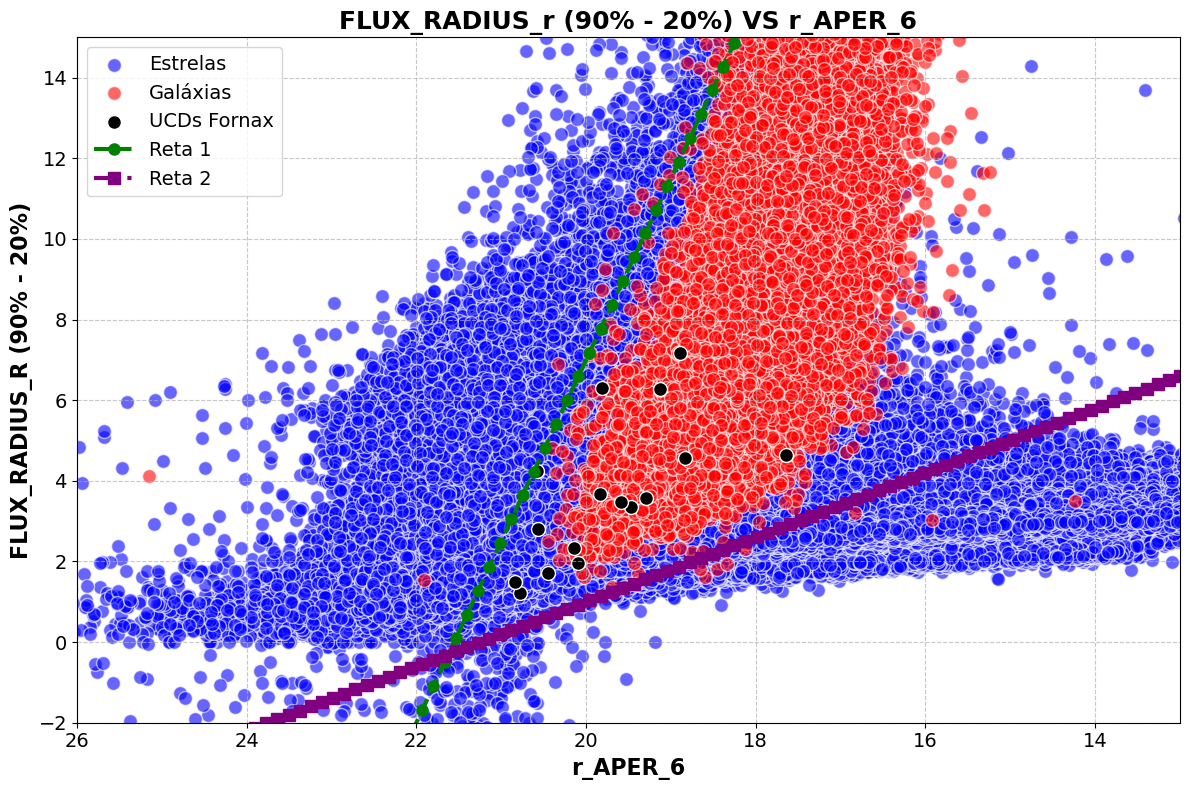
\includegraphics[width=0.8\columnwidth,angle=0]{f_90_20_R_APER_6.png}
    \caption{Gráfico de \text{FLUX\_RADIUS\_90} - \text{FLUX\_RADIUS\_20} em função de \text{r\_APER\_6} para objetos da amostra com classificação estrela-galáxia do GAIA DR3 com probabilidade maior que 90\%. Pontos em azul representam as estrelas, em vermelho as galáxias e em preto as UCDs. As retas em verde e roxo representam os cortes para remover a contaminação de estrelas.}
    \label{flux_radius_1}
    \end{center}
\end{figure}

\begin{figure}[!ht]
    \begin{center}
    % \setcaptionmargin{1cm}
    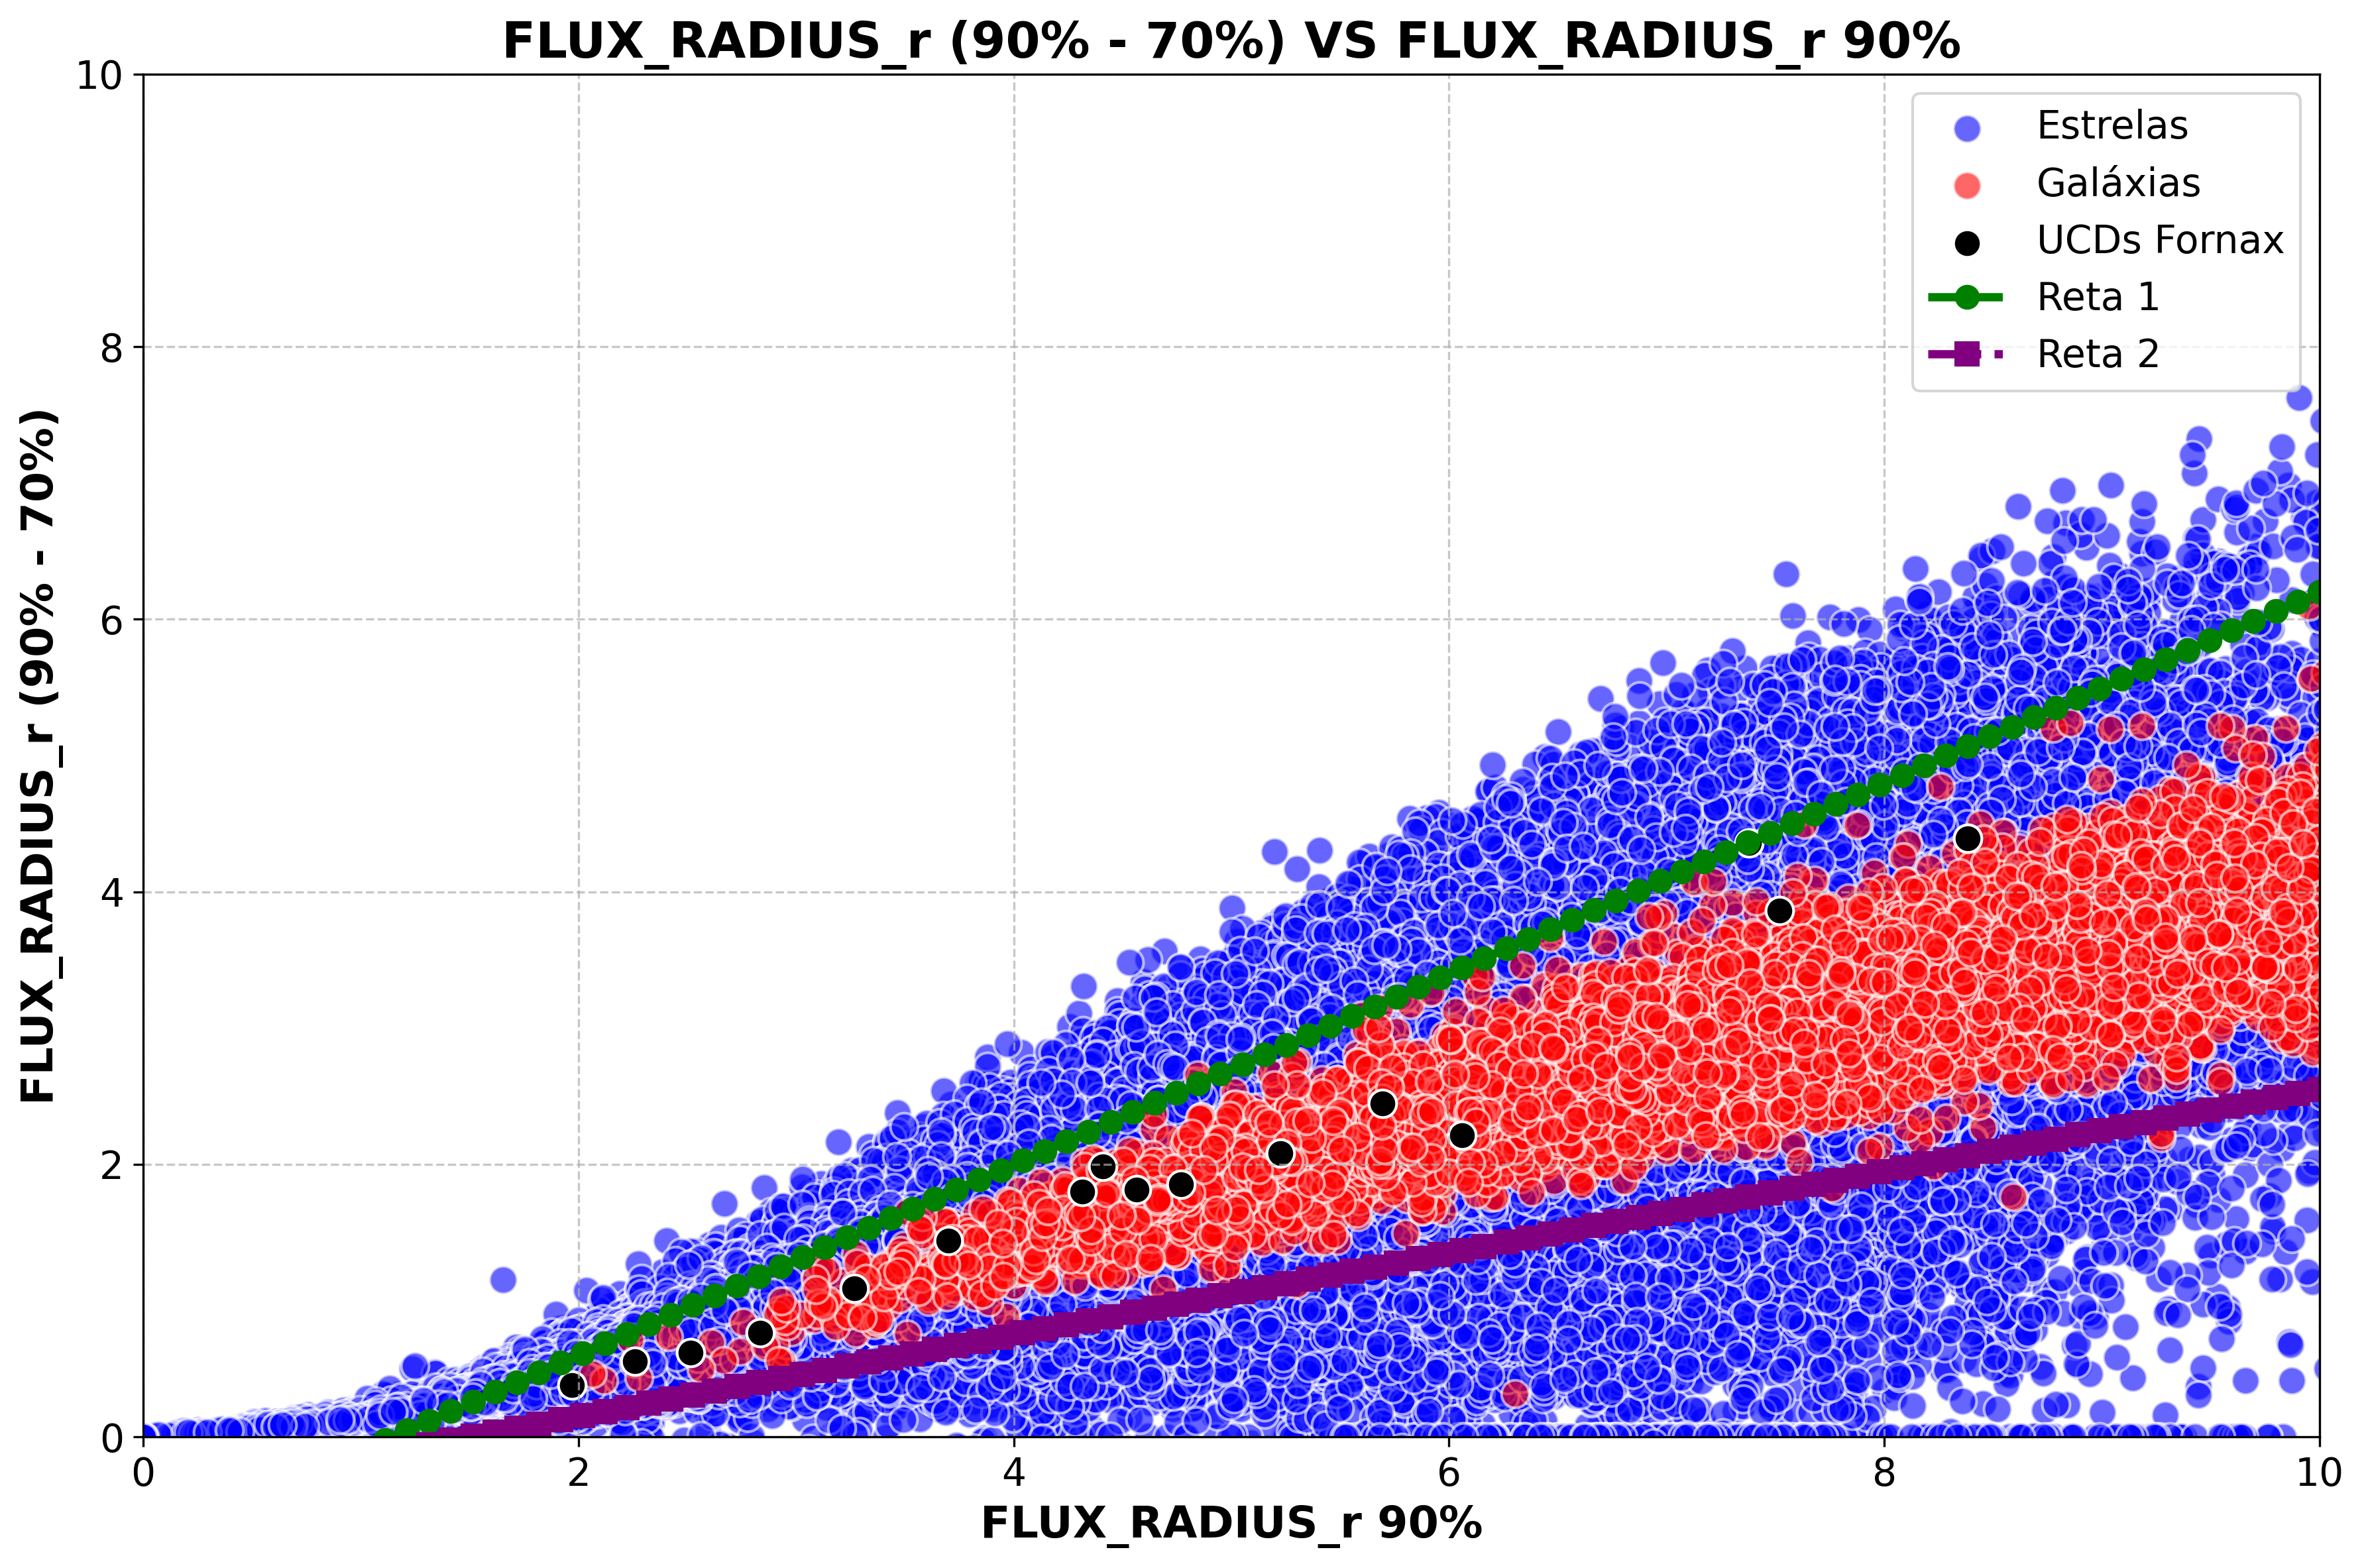
\includegraphics[width=0.8\columnwidth,angle=0]{f_90_70_FLUX_RADIUS_90_R.png}
    \caption[]{Gráfico de \text{FLUX\_RADIUS\_90} - \text{FLUX\_RADIUS\_70} em função de \text{FLUX\_RADIUS\_90} para objetos da amostra com classificação estrela-galáxia do GAIA DR3 com probabilidade maior que 90\%. Pontos em azul representam as estrelas, em vermelho as galáxias e em preto as UCDs. As retas em verde e roxo representam os cortes para remover a contaminação de estrelas.}
    \label{flux_radius_2}
    \end{center}
\end{figure}

\begin{figure}[!ht]
    \begin{center}
    % \setcaptionmargin{1cm}
    \includegraphics[width=0.8\columnwidth,angle=0]{f_70_20_f_90_70.png}
    \caption[]{Gráfico de \text{FLUX\_RADIUS\_70} - \text{FLUX\_RADIUS\_20} em função de \text{FLUX\_RADIUS\_90} - \text{FLUX\_RADIUS\_70} para objetos da amostra com classificação estrela-galáxia do GAIA DR3 com probabilidade maior que 90\%. Pontos em azul representam as estrelas, em vermelho as galáxias e em preto as UCDs. As retas em verde e roxo representam os cortes para remover a contaminação de estrelas.}
    \label{flux_radius_3}
    \end{center}
\end{figure}

Após esses cortes, ficamos com uma amostra de 202.870 objetos. Para seleção de objetos compactos, com base nas classificações do modelo, filtramos aqueles com probabilidade maior que 90\% de serem extensos. A partir dessa amostra, selecionamos as candidatas a UCDs, que são objetos compactos com alta probabilidade de serem extensos, resultando em 9.918 objetos.

Fazendo uso das previsões de redshifts fotométricos da seção \ref{sec:zphot}, iremos cortar os objetos com redshifts fotométricos vindos de \citep{erik_photoz_2024}, que são mais robustos que o nosso modelo de redshift. Já para os objetos que não têm redshifts fotométricos disponíveis, iremos usar o mesmo corte, mas para o nosso modelo de regressão de redshifts fotométricos. O corte adotado para o redshift fotométrico é feito para removermos objetos com maiores chances de serem do fundo, e dado os erros do modelo, principalmente para os objetos mais próximos, usaremos um corte mais conservador. Assim, adotamos um corte para os redshifts fotométricos de \textit{$z_{phot}$}$\leq$0.05, que corresponde a um valor de uma ordem de magnitude acima do redshift de Fornax.

Ao final de todo o processo de seleção de candidatas com maiores similaridades com as UCDs, encontramos um total de 242 objetos de uma amostra inicial de aproximadamente 2,9 milhões de objetos no campo de Fornax. O resultado gerado até aqui inclui cortes adotados pelo nosso modelo de classificação, sendo possível replicar o processo para outras amostras de dados. Com essa amostra de candidatas, que representa uma fração menor, porém ainda significativa, podemos partir para uma análise um pouco mais detalhada desses objetos, de maneira a selecionar apenas uma dezena para observação espectroscópica.

Como já comentado, a classificação estrela-galáxia do GAIA DR3 é útil, porém temos que tomar cuidado, ainda mais para os objetos mais pontuais, sem movimento próprio medido e com magnitudes mais altas do que as atingidas pelo GAIA. Um dos problemas é que o GAIA tem maior precisão para objetos com magnitudes até aproximadamente $r \sim 18$, o que pode levar a classificações menos confiáveis para objetos mais fracos. Assim, não tínhamos aplicado o corte em uma primeira análise, mas com nossa amostra final, aplicaremos um corte do classificador estelar, para encontrarmos aqueles mais interessantes que mesmo o GAIA classificou como galáxia. Assim, selecionamos aqueles com probabilidade menor que 0.5 de serem estrelas.

Desses objetos, obtivemos uma amostra de 10 candidatos. Observando as imagens dos objetos no Legacy Survey, notamos que parte dos objetos tem uma aparência mais extensa, e mesmo com os valores de \textit{FWHM} menores, apresentam parte de um disco ou braços espirais, e que podem ser objetos de fundo. Assim, escolhemos desses objetos aqueles que têm uma aparência mais pontual, com um critério visual, sem uma segunda componente extensa além do núcleo, selecionando 1 candidata. 

% Selecionamos também mais uma galáxia que, mesmo sendo um pouco mais extensa, está perto de uma galáxia massiva de Fornax, sendo interessante para estudos futuros.

Do restante da amostra de candidatas, com objetos mais fracos, que esperamos que o classificador estelar do GAIA DR3 tenha mais dificuldade em classificar, assim como as UCDs conhecidas mais fracas vistas na Figura \ref{distribuicao_fwhm_image_r_r_aper6_ucds_fornax}, esperamos também encontrar objetos interessantes. Para um critério mais objetivo, fizemos uso do outro classificador galáxia-estrela-quasar do S-PLUS DR4 (\textit{PROB\_GAL}, \textit{PROB\_STAR}, \textit{PROB\_QSO}) \citep{lili_classification}\footnote{Documentação S-PLUS Data Release 5: \url{https://splus.cloud/documentation/idr5}}. Ele oferece uma classificação levando em conta as bandas fotométricas do S-PLUS.

Selecionamos assim os objetos que não foram selecionados pelo corte estelar do GAIA DR3, mas que foram classificados com probabilidade acima de 80\% de ser galáxias pelo S-PLUS DR4. Dessa seleção foram retornados 13 objetos.

Tínhamos 217 objetos na nossa amostra de candidatas, dos quais selecionamos 1 interessante pela classificação de galáxia do GAIA DR3, e mais 13 pela classificação de galáxia do S-PLUS DR4. Assim, temos um total de 14 objetos para a amostra final de candidatas a UCDs em Fornax.

Comparando-os com as UCDs conhecidas, apresentamos na Figura \ref{ucds_and_candiadates_star_cut_photospec} dois gráficos de fotoespectros sobrepostos: o primeiro mostra as UCDs conhecidas, enquanto o segundo exibe os objetos selecionados como candidatas.

\begin{figure}[!ht]
    \centering
    \captionsetup{justification=centering}
    \begin{subfigure}[b]{0.95\textwidth}
        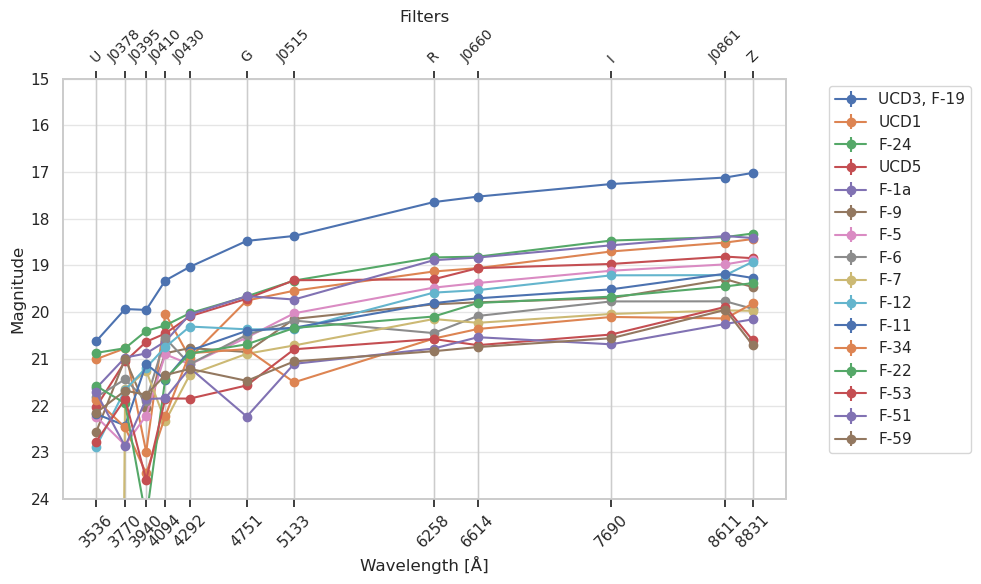
\includegraphics[width=\textwidth]{photo_specs/photospec_ucds.png}
        \caption{Fotoespectros das UCDs conhecidas em Fornax}
    \end{subfigure}
    \begin{subfigure}[b]{0.95\textwidth}
        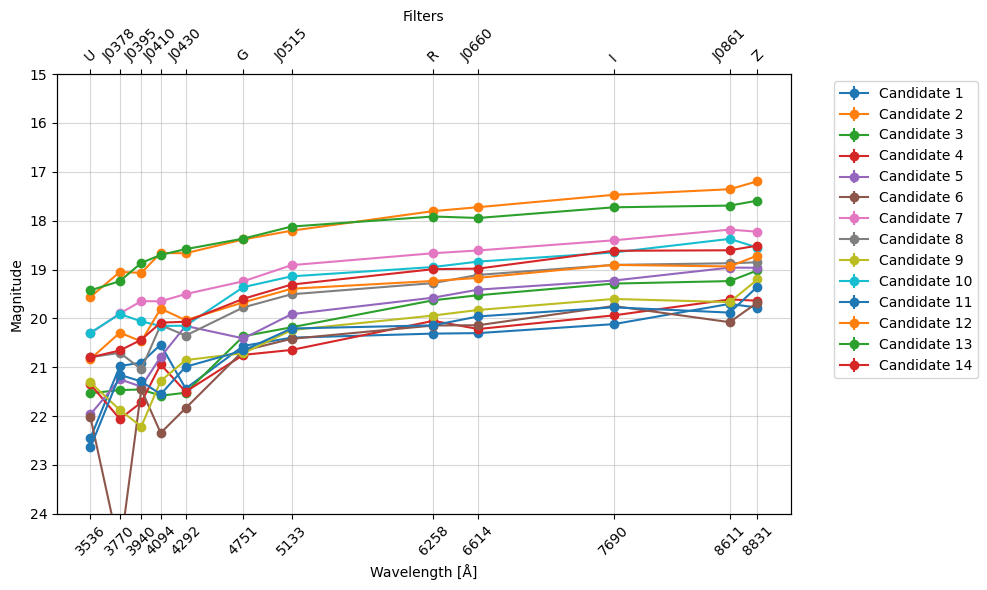
\includegraphics[width=\textwidth]{photo_specs/photospec_candidatas.png}
        \caption{Fotoespectros dos objetos selecionados para candidatas a UCD}
    \end{subfigure}
    \caption{Gráficos de fotoespectros sobrepostos das UCDs conhecidas em Fornax e dos objetos selecionados da amostra de candidatas.}
    \label{ucds_and_candiadates_star_cut_photospec}
\end{figure}


Apresentamos na Figura \ref{ucds_candidates_final_imagens} as imagens dos 14 objetos selecionados como candidatas a UCDs em Fornax.

\begin{figure}[!ht]
    \centering
    \captionsetup{justification=centering}
    \begin{subfigure}[b]{0.25\textwidth}
        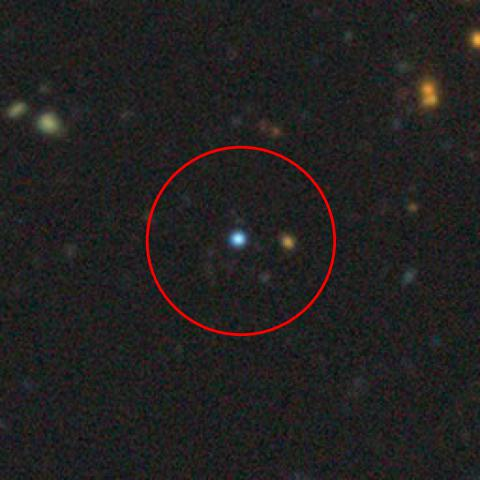
\includegraphics[width=\textwidth]{candidata_final/01.jpg}
        \caption{Candidata 01}
    \end{subfigure}
    \begin{subfigure}[b]{0.25\textwidth}
        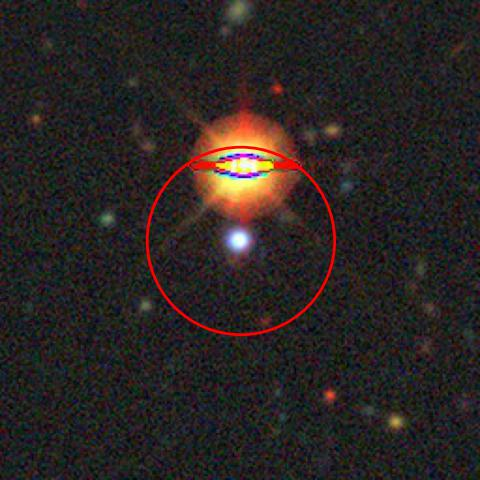
\includegraphics[width=\textwidth]{candidata_final/02.jpg}
        \caption{Candidata 02}
    \end{subfigure}
    \begin{subfigure}[b]{0.25\textwidth}
        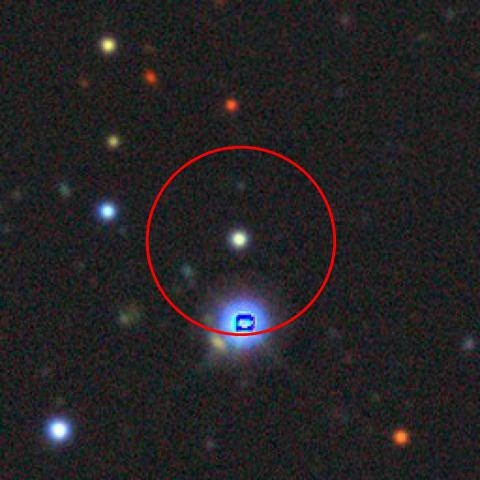
\includegraphics[width=\textwidth]{candidata_final/03.jpg}
        \caption{Candidata 03}
    \end{subfigure}
    \begin{subfigure}[b]{0.25\textwidth}
        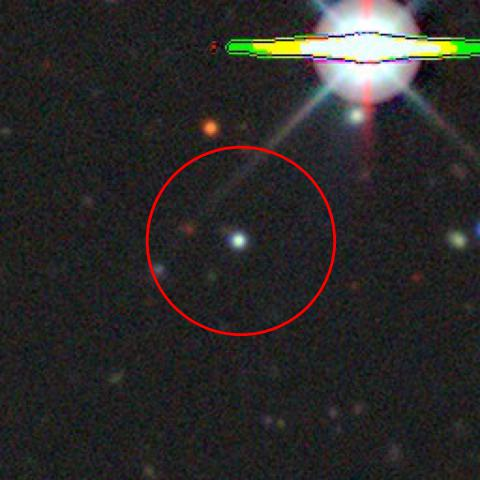
\includegraphics[width=\textwidth]{candidata_final/04.jpg}
        \caption{Candidata 04}
    \end{subfigure}
    \begin{subfigure}[b]{0.25\textwidth}
        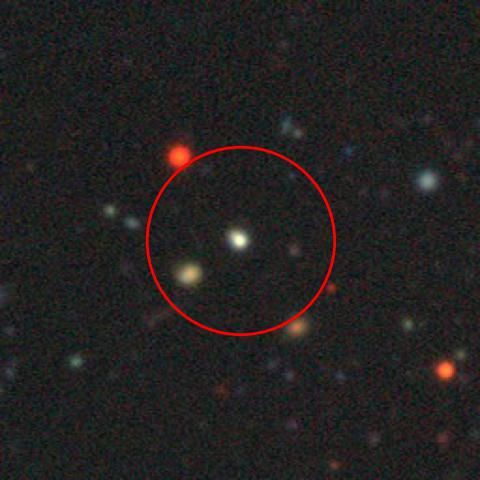
\includegraphics[width=\textwidth]{candidata_final/05.jpg}
        \caption{Candidata 05}
    \end{subfigure}
    \begin{subfigure}[b]{0.25\textwidth}
        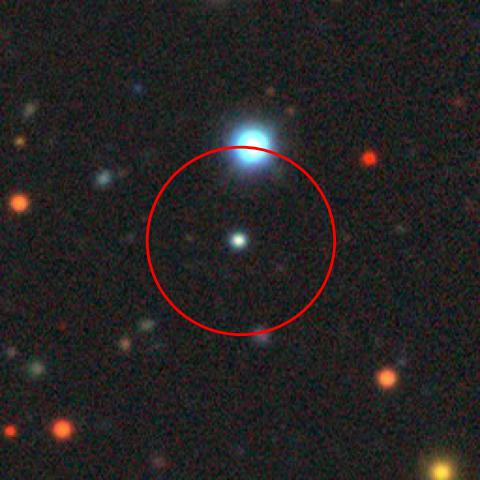
\includegraphics[width=\textwidth]{candidata_final/06.jpg}
        \caption{Candidata 06}
    \end{subfigure}
    \begin{subfigure}[b]{0.25\textwidth}
        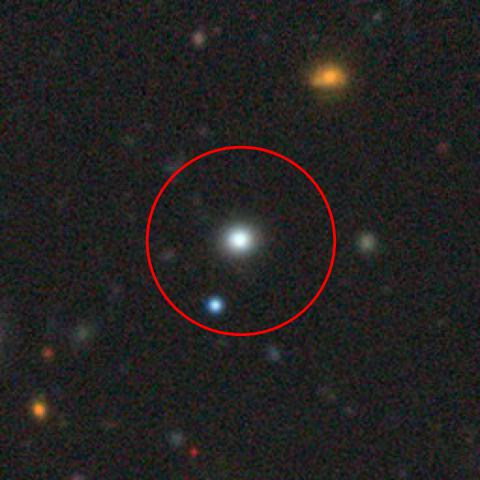
\includegraphics[width=\textwidth]{candidata_final/07.jpg}
        \caption{Candidata 07}
    \end{subfigure}
    \begin{subfigure}[b]{0.25\textwidth}
        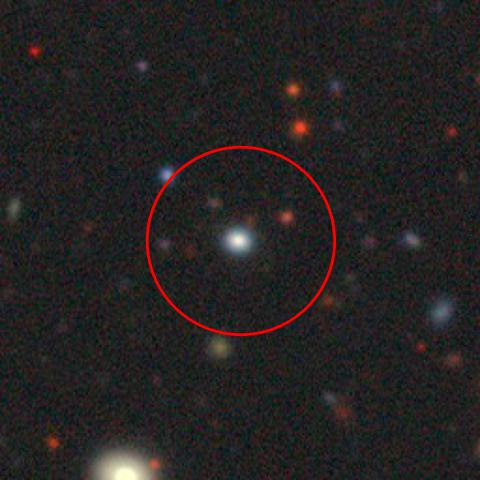
\includegraphics[width=\textwidth]{candidata_final/08.jpg}
        \caption{Candidata 08}
    \end{subfigure}
    \begin{subfigure}[b]{0.25\textwidth}
        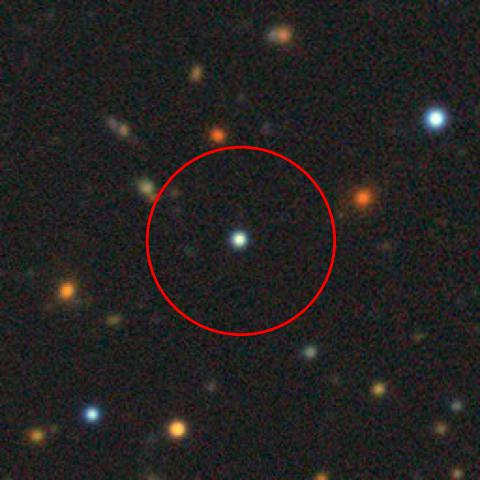
\includegraphics[width=\textwidth]{candidata_final/09.jpg}
        \caption{Candidata 09}
    \end{subfigure}
    \begin{subfigure}[b]{0.25\textwidth}
        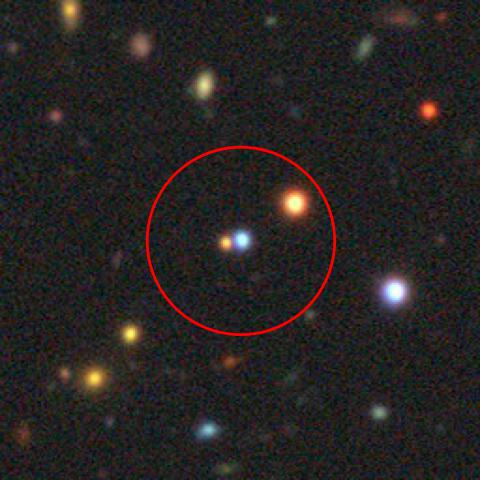
\includegraphics[width=\textwidth]{candidata_final/10.jpg}
        \caption{Candidata 10}
    \end{subfigure}
    \begin{subfigure}[b]{0.25\textwidth}
        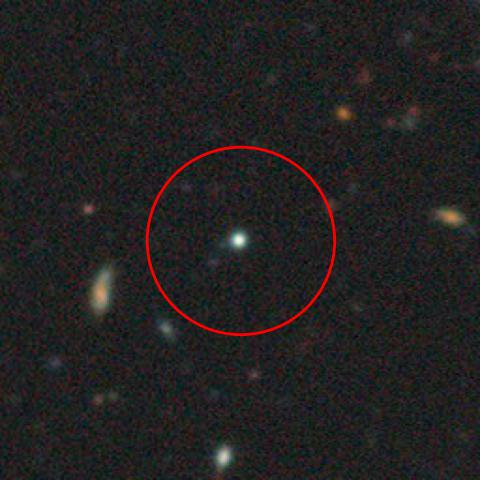
\includegraphics[width=\textwidth]{candidata_final/11.jpg}
        \caption{Candidata 11}
    \end{subfigure}
    \begin{subfigure}[b]{0.25\textwidth}
        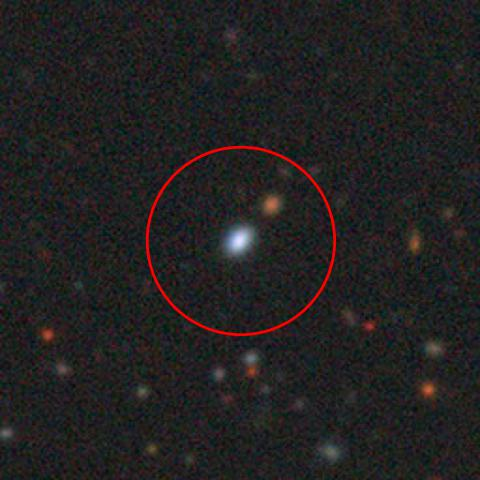
\includegraphics[width=\textwidth]{candidata_final/12.jpg}
        \caption{Candidata 12}
    \end{subfigure}
    \begin{subfigure}[b]{0.25\textwidth}
        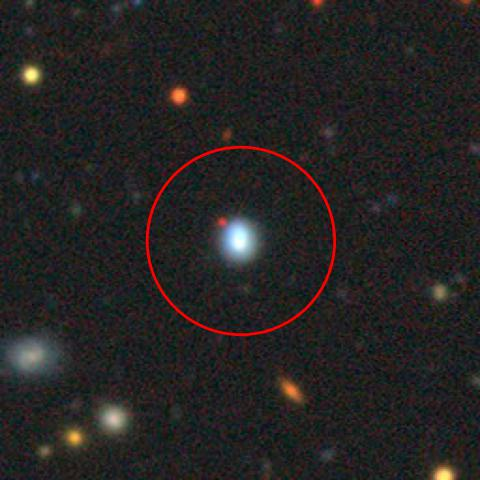
\includegraphics[width=\textwidth]{candidata_final/13.jpg}
        \caption{Candidata 13}
    \end{subfigure}
    \begin{subfigure}[b]{0.25\textwidth}
        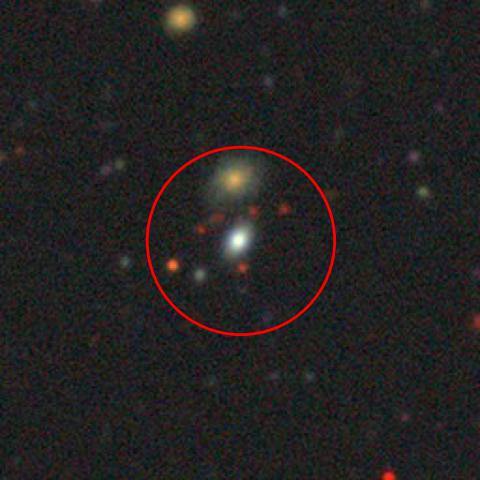
\includegraphics[width=\textwidth]{candidata_final/14.jpg}
        \caption{Candidata 14}
    \end{subfigure}
    \caption[]{Imagens das candidatas finais a UCDs. Imagens obtidas pelo Legacy Survey.}
    \label{ucds_candidates_final_imagens}
\end{figure}



\section{Análise das candidatas}\label{sec:analise_candidatas}
Selecionamos 14 objetos para a amostra final de candidatas a UCDs da seção \ref{cap:selecao_candidatas}.
%  mais 4 objetos com possíveis sinais de emissão da subseção \ref{subsec: candidatas_emissao}, totalizando 21 objetos.

Utilizando o catálogo de Fornax proveniente do projeto S-PLUS Fornax \citep{castelli2024splusfornaxprojectsfp}, com a fotometria apresentada por \citep{haack2024splusfornaxprojectsfp}, obtivemos uma amostra de galáxias conhecidas, classificadas morfologicamente. Com base nisso, realizamos uma análise das candidatas selecionadas, comparando-as com as galáxias conhecidas. Identificamos, em diversos conjuntos de parâmetros, tanto a localização das UCDs reais quanto a posição das nossas candidatas.

Selecionamos as categorias morfológicas de galáxias mais relevantes com as maiores quantidades de objetos para comparação. Dentre elas, temos as galáxias anãs elípticas, nucleadas e não nucleadas, junto das irregulares. Outros tipos importantes incluem as LSB (Low Surface Brightness) e as galáxias espirais.

Analisamos como as UCDs e as galáxias conhecidas, classificadas morfologicamente, se distribuem em diferentes espaços de parâmetros, especialmente aqueles que representam a morfologia de objetos compactos. Um dos parâmetros avaliados foi o brilho superficial médio, aqui calculado na banda $r$, que mede a densidade superficial de luminosidade média de um objeto. Ele foi obtido a partir da magnitude aparente e do raio efetivo do objeto.

Utilizamos o parâmetro \textit{PETRO\_RADIUS}, fornecido pelo SExtractor, que está em unidades dos semieixos \textit{A} e \textit{B}, para calcular o raio do objeto em cada um dos dois semieixos. A partir disso, determinamos o brilho superficial médio, somando a magnitude aparente a 2,5 vezes o logaritmo da área da elipse, convertida para unidades de arcsec$^2$ (multiplicando pelo fator de 0,55 arcsec/pixel para cada semieixo). A equação utilizada para o cálculo do brilho superficial médio é:

\begin{equation}
    \mu_{\text{medio}} = \text{mag\_aparente} + 2.5 \times \log_{10}(\pi \times A \times B \times 0.55^2 \times \text{PETRO\_RADIUS}^2)
    \label{equation_sb}
\end{equation}

Na Figura \ref{sb_r_ucds_galaxias}, mostramos a distribuição do brilho superficial médio na banda $r$ para as UCDs conhecidas e as galáxias morfologicamente classificadas, juntamente com as candidatas selecionadas.

\begin{figure}[!ht]
    \begin{center}
    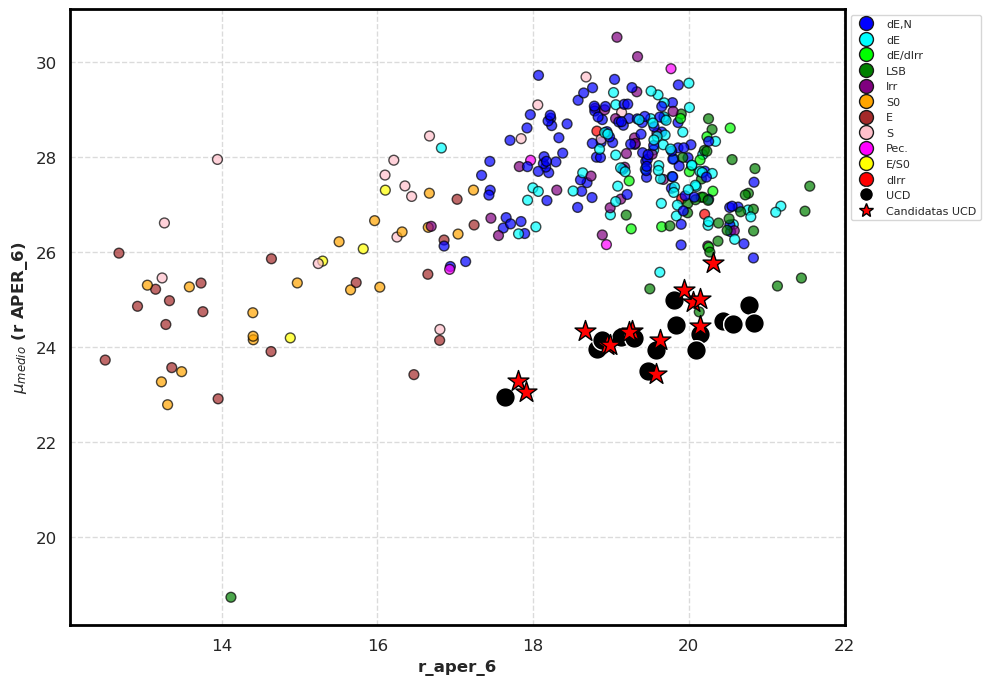
\includegraphics[width=1.\columnwidth,angle=0]{sb_r_ucds_galaxias.png}
    \caption[]{Gráfico da magnitude superficial média na banda $r$ em função da magnitude aparente na banda $r$ para as UCDs conhecidas, as galáxias morfologicamente classificadas e as candidatas selecionadas.}
    \label{sb_r_ucds_galaxias}
    \end{center}
\end{figure}

A Figura \ref{sb_r_ucds_galaxias} mostra que, para parte das galáxias com morfologia conhecida apresentadas, elas seguem uma distribuição em cauda para o brilho superficial médio na banda $r$, em função da magnitude aparente na banda $r$. Para as UCDs conhecidas e as candidatas, elas estão localizadas na parte inferior. Esse fato mostra que, para um mesmo brilho superficial médio, as UCDs e as candidatas são menos brilhantes que as galáxias de morfologia apresentada, que são mais extensas. 

Tanto para os cenários previstos de formação das UCDs como núcleos expostos de galáxias anãs que foram despojadas de suas camadas externas por interações gravitacionais em aglomerados, quanto para aqueles de formação a partir de aglomerados estelares massivos, o resultado são objetos com alta densidade estelar e raios efetivos pequenos

Nesse tipo de diagrama, quando comparado com as galáxias de morfologia “convencional” (elípticas, espirais, etc.), essa diferença estrutural dos dois tipos é evidenciada: as UCDs ocupam uma região “compacta e luminosa” para seu tamanho, enquanto as galáxias seguem uma correlação mais “espalhada” entre luminosidade e tamanho/brilho superficial.

Na Figura \ref{r_aper_6_mu_max} e \ref{r_aper_6_kron_radius}, temos os parâmetros \textit{MU\_MAX} e \textit{KRON\_RADIUS}, respectivamente, ambos em função da magnitude aparente na banda $r$. O \textit{MU\_MAX} representa o pico de brilho superficial do objeto, indicando o quão brilhante é a região mais intensa do objeto em comparação com o fundo. Já o \textit{KRON\_RADIUS} (raio de Kron) é o raio principal de medição definido pelo SExtractor para estimar a magnitude total. Ele é calculado com base na distribuição de luz do objeto, usando o fluxo integrado ao longo de elipses que seguem o perfil de brilho do mesmo objeto.

Em ambas as figuras, observamos que as candidatas se localizam em regiões mais próximas das UCDs conhecidas do que das demais galáxias com morfologia apresentada. Na Figura \ref{r_aper_6_mu_max}, vemos que elas seguem uma segunda curva abaixo das galáxias mais extensas. Já para a Figura \ref{r_aper_6_kron_radius}, vemos que, conforme os objetos ficam mais fracos, o raio de Kron aumenta. Quando um objeto é mais extenso ou tem a luz distribuída de forma difusa, a ferramenta precisa usar um raio maior para abranger boa parte do fluxo total. Em outras palavras, objetos mais fracos (mas espalhados em área maior) resultam em um Kron Radius maior, pois o algoritmo “enxerga” a luz se estendendo além de um núcleo compacto. Já objetos brilhantes e concentrados apresentam Kron Radius menor, pois a maior parte do fluxo está contida numa região pequena. Ainda assim, notamos que as candidatas selecionadas e UCDs conhecidas têm a mesma tendência, porém agrupadas em uma região mais abaixo do gráfico.

\begin{figure}[!ht]
    \begin{center}
    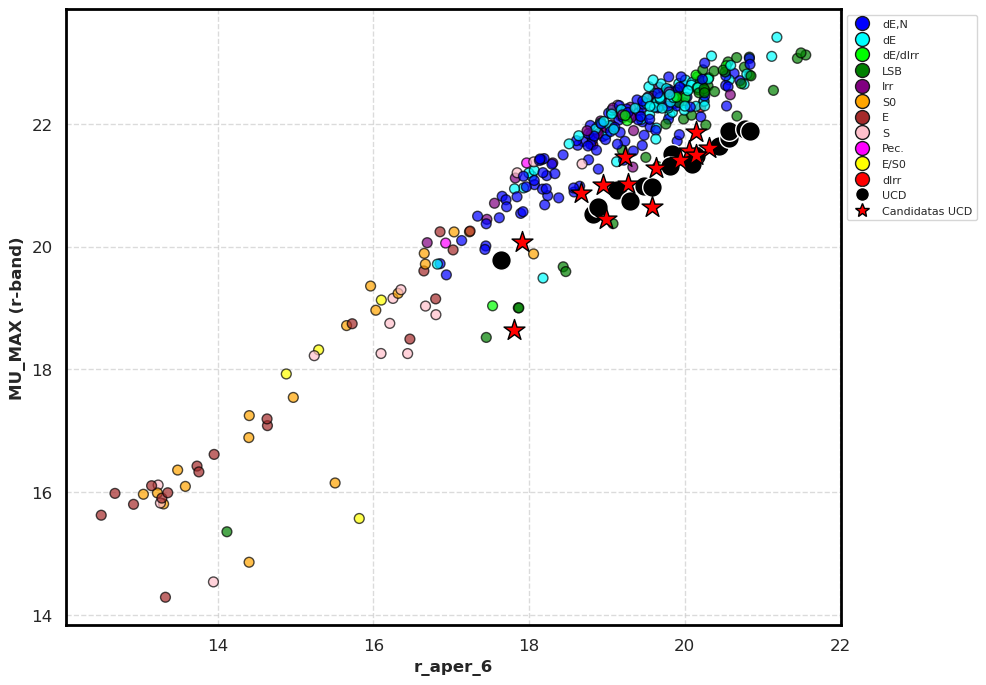
\includegraphics[width=1.\columnwidth,angle=0]{r_aper_6_mu_max.png}
    \caption[]{Gráfico do parâmetro \textit{MU\_MAX} em função da magnitude aparente na banda $r$ para as UCDs conhecidas, as galáxias morfologicamente classificadas e as candidatas selecionadas.}
    \label{r_aper_6_mu_max}
    \end{center}
\end{figure}


\begin{figure}[!ht]
    \begin{center}
    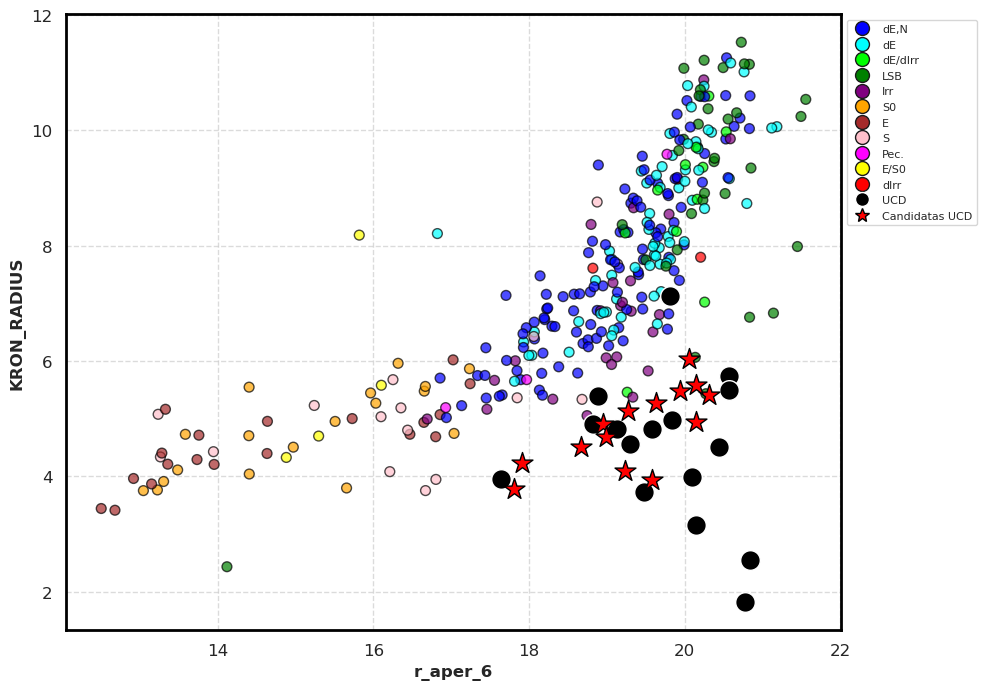
\includegraphics[width=1.\columnwidth,angle=0]{r_aper_6_kron_radius.png}
    \caption[]{Gráfico do parâmetro \textit{KRON\_RADIUS} em função da magnitude aparente na banda $r$ para as UCDs conhecidas, as galáxias morfologicamente classificadas e as candidatas selecionadas.}
    \label{r_aper_6_kron_radius}
    \end{center}
\end{figure}


Mostramos na Figura \ref{distribuicao_candidatas_radec} a distribuição em coordenadas equatoriais das candidatas selecionadas, juntamente com as UCDs conhecidas e o compilado das galáxias massivas descritas na seção \ref{subsec:galaxias_massivas}.

\begin{figure}[!ht]
    \begin{center}
    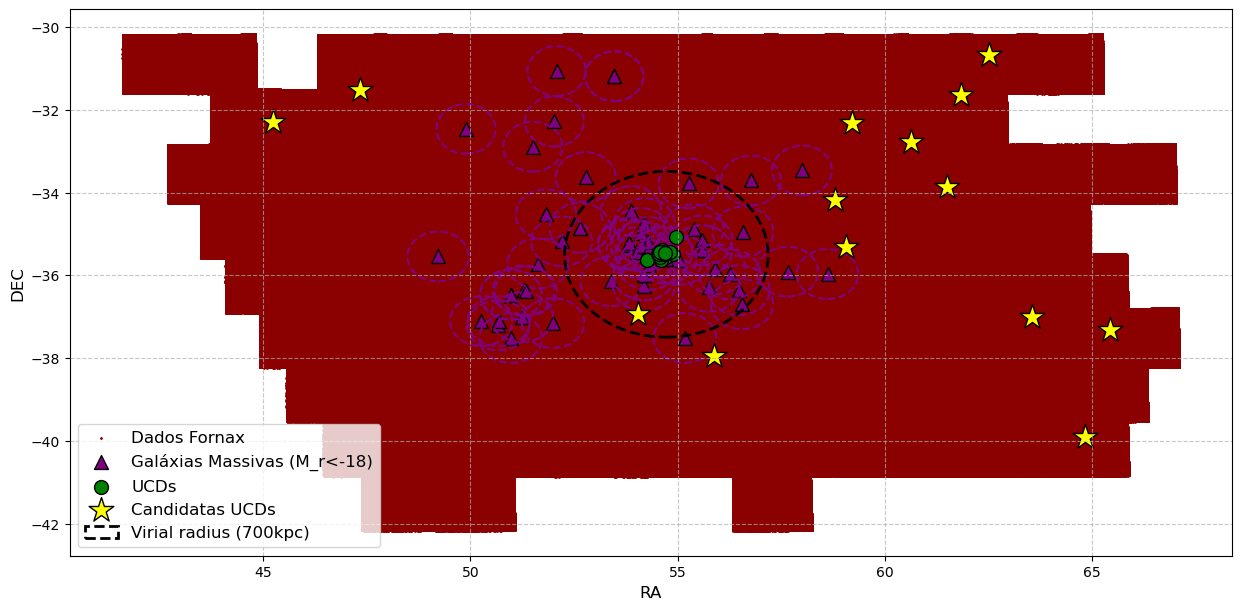
\includegraphics[width=1.\columnwidth,angle=0]{distribuicao_candidatas_radec.png}
    \caption[]{Distribuição em coordenadas equatoriais (RA, DEC) das candidatas a UCDs selecionadas (estrelas azuis), comparadas com as UCDs conhecidas (círculos verdes) e as galáxias massivas (triângulos roxos) no aglomerado de Fornax. O fundo vermelho representa a área de cobertura dos dados do S-PLUS. Os círculos tracejados em roxo indicam um raio de 200 kpc ao redor de cada galáxia massiva. O arco preto corresponde ao raio de virial do aglomerado (700 kpc), enquanto o arco cinza representa o raio de 349 kpc.}
    \label{distribuicao_candidatas_radec}
    \end{center}
\end{figure}



